\documentclass[12pt]{article}

\usepackage[
  top=5mm,
  bottom=5mm,
  left=5mm,
  right=5mm,
  marginparwidth=0mm,
  marginparsep=0mm,
  headheight=15pt,
  centering,
  includefoot,
  includehead
]{geometry}
\usepackage{multicol}
\usepackage{tabularx}
\usepackage{hyperref}

\hypersetup{
    colorlinks=false,
    linktoc=all,
}

% preamble
\usepackage{amssymb}
\usepackage{amsmath, amsthm}
\usepackage{xcolor}
\usepackage{fancyhdr}
\usepackage{enumitem}
\usepackage{mathtools}
\usepackage{framed}
\usepackage{parskip}
\usepackage{graphicx}
\usepackage{chngcntr}
\usepackage{float}
\usepackage{listings}
\usepackage{inconsolata}
\usepackage{transparent}
\usepackage{tikz}


% \input xypic (for commutative diagrams)
% \include{mssymb}

\def\A{{\mathbb A}}
\def\P{{\mathbb P}}
\def\N{{\mathbb N}}
\def\Z{{\mathbb Z}}
\def\Q{{\mathbb Q}}
\def\R{{\mathbb R}}
\def\C{{\mathbb C}}
\def\F{{\mathbb F}}
\def\O{{\cal O}}
\let\sec\S
\let\S\relax
\def\S{{\mathfrak S}}
\def\g{{\mathfrak g}}
\def\p{{\mathfrak p}}
\def\h{{\mathfrak h}}
\def\n{{\mathfrak n}}
\def\v{{\mathfrak v}}
\def\m{{\mathfrak m}}
\def\a{{\alpha}}


\newcommand{\skipline}{\vspace{\baselineskip}}
\newcommand{\dis}{\displaystyle}
\newcommand{\noin}{\noindent}


% remove all paragraph indents
\setlength{\parindent}{0pt}

% Figure counter include section
\counterwithin{figure}{section}

% Cleaner figures
\newcommand{\fig}[3][0.4]{
  \begin{figure}[H]
    \centering
    \includegraphics[width=#1\textwidth, keepaspectratio]{#2}
    \caption{#3}
  \end{figure}
}

% Parens, Brackets, Bars, and Braces
\newcommand{\parens}[1]{ \left(#1\right) }
\newcommand{\bracks}[1]{ \left[#1\right] }
\newcommand{\braces}[1]{ \left\{#1\right\} }
\newcommand{\abs}[1]{ \left|#1\right| }
\newcommand{\floor}[1]{ \left\lfloor#1\right\rfloor }
\newcommand{\ceil}[1]{ \left\lceil#1\right\rceil }

% Mathematical notation


\newcommand{\Span}{\mathrm{Span}}
\newcommand{\Range}{\mathrm{Range}}
\newcommand{\Null}{\mathrm{Null}}
\newcommand{\Rank}{\mathrm{Rank}}
\newcommand{\rank}{\mathrm{rank}}
\newcommand{\Nullity}{\mathrm{Nullity}}
\newcommand{\nullity}{\mathrm{nullity}}
\newcommand{\longhookrightarrow}{\lhook\joinrel\relbar\joinrel\rightarrow}
\newcommand{\la}{\leftarrow}
\newcommand{\ra}{\rightarrow}
\newcommand{\La}{\Leftarrow}
\newcommand{\Ra}{\Rightarrow}
\newcommand{\dbar}{\overline{\partial}}
\newcommand{\gequ}{\geqslant}
\newcommand{\lequ}{\leqslant}
\newcommand{\Hom}{\mathrm{Hom}}
\newcommand{\End}{\mathrm{End}}
\newcommand{\Aut}{\mathrm{Aut}}
\newcommand{\Coker}{\mathrm{Coker}}
\newcommand{\Row}{\mathrm{Row}}
\newcommand{\Ker}{\mathrm{Ker}}
\newcommand{\Tr}{\mathrm{Tr}}
\newcommand{\Id}{\mathrm{Id}}
% \newcommand{\mod}{\mathrm{mod }}
\newcommand{\un}{\underline}
\newcommand{\ov}{\overline}
\newcommand{\wt}{\widetilde}
\newcommand{\wh}{\widehat}
\newcommand{\pr}{\prime}
\newcommand{\rk}{\mathrm{rk}}
\newcommand{\im}{\mathrm{Im}}

% Linear Algebra

\newcommand{\lind}{linearly independent}
\newcommand{\ldep}{linearly dependent}
\renewcommand{\vec}[1]{
  {\bf #1}
}
\newcommand{\lincomb}[3]{
  #1_{1}#2_{1} + #1_{2}#2_{2} + \cdots + #1_{#3}#2_{#3}
}
\newcommand{\neglincomb}[3]{
  -#1_{1}#2_{1} - #1_{2}#2_{2} - \cdots - #1_{#3}#2_{#3}
}
\newcommand{\constants}[2]{
  #1_{1}, #1_{2}, \cdots, #1_{#2}
}
\newcommand{\constantsz}[2]{
  #1_{0}, \constants{#1}{#2}
}

% Analysis
\newcommand{\limfty}[1]{\lim_{#1 \to \infty}}
\newcommand{\seq}[2]{\{#1_{#2}\}_{#2 \in \N}}
\newcommand{\sseq}[3]{\{#1_{#2_{#3}}\}_{#3 \in \N}}
\newcommand{\chep}{Let $\epsilon > 0$}

% Category Theory
\newcommand{\catC}{\mathcal{C}}
\newcommand{\catD}{\mathcal{D}}
\newcommand{\functF}{\mathcal{F}}
\newcommand{\functG}{\mathcal{G}}
\newcommand{\functI}{\mathcal{I}}
\newcommand{\functU}{\mathcal{U}}

\newcommand{\op}[1]{#1^{\mathrm{op}}}
\newcommand{\Obj}{\mathrm{Obj}}

\newcommand{\Set}{\mathbf{Set}}
\newcommand{\Grp}{\mathbf{Grp}}
\newcommand{\Top}{\mathbf{Top}}
\newcommand{\cRing}{\mathbf{cRing}}
\newcommand{\BanAnaMan}{\mathbf{BanAnaMan}}
\newcommand{\FinSet}{\mathbf{FinSet}}
\newcommand{\Vect}{\mathbf{Vect}}
\newcommand{\Two}{\mathbf{2}}


% ================= %
% Headers & Footers
% ================= %
\pagestyle{fancy}
\fancyhf{}
\newcommand{\intros}[3]{
  \lhead{\textbf{#1} {#2}}
  \rhead{#3}}
\rfoot{\thepage}
\renewcommand{\headrulewidth}{0pt}



% ================= %
%       Utils
% ================= %
\newcommand{\induction}[3]{
  \textbf{Base Case}. #1 \\
  \textbf{Inductive Hypothesis}. \\ #2 \\
  \textbf{Inductive Step}. \\ #3
}



% Used to list all problems on homework
\newcommand{\problems}[1]{
  \medskip \noin
  {\bf Problems}

  #1

  \medskip{}
}


% When prof does Question/Answer styling
\newcommand{\qna}[2]{
  {\bf Question} #1

  \medskip

  {\bf Answer} #2
}


% augmented matrices
\makeatletter
\renewcommand*\env@matrix[1][*\c@MaxMatrixCols c]{%
  \hskip -\arraycolsep
  \let\@ifnextchar\new@ifnextchar
  \array{#1}}
\makeatother

% ================= %
%      Box Meta
% ================= %

% #2 - FG Color
% #3 - BG Color
\newenvironment{fancyleftbar}[3][\hsize]
{%
    \def\FrameCommand
    {%
        {\color{#2}\vrule width 3pt}%
        \hspace{0pt}%must no space.
        \fboxsep=\FrameSep\colorbox{#3}%
    }%
    \MakeFramed{\hsize#1\advance\hsize-\width\FrameRestore}%
}
{\endMakeFramed}

\newenvironment{simpleleftbar}[3][\hsize]
{%
    \def\FrameCommand
    {%
        {\vrule width 0.5pt}%
        \hspace{3pt}
        \fboxsep=\FrameSep%
    }%
    \MakeFramed{\hsize#1\advance\hsize-\width\FrameRestore}%
}
{\endMakeFramed}

% Used to allow the color argument to pass through the environment%
\newsavebox{\boxqed} 

% #1 - Header
% #2 - FG Color
% #3 - BG Color
\newenvironment{fancybox}[3]{
  \sbox\boxqed{\textcolor{#2}{$\blacksquare$}}
  \begin{fancyleftbar}{#2}{#3}

  \noin
  #1
  % {\large \bf \underline{#1}}
  \smallskip\noin \\
}
{

  \medskip
  \noin
  \usebox\boxqed

  \end{fancyleftbar}
}

% #1 - Text header
% #2 - Outer Text
% #3 - Inner Text
% #4 - Inner Header
% #5 - FG Color
% #6 - Background Color
\newcommand{\boxmeta}[6]{
  #1
  % {\small\sc\uppercase{#1}}

  #2

  \begin{fancybox}{#4}{#5}{#6}
    \noin
    #3
  \end{fancybox}
}

% #1 - Title
% #2 - FG Color
% #3 - BG Color
% #4 - Inner Text
\newcommand{\baronly}[4]{
  \begin{simpleleftbar}{#2}{#3}
    {\bf #1}.

    #4
  \end{simpleleftbar}
}

% ================= %
%     Box Colors
% ================= %

\definecolor{theorem_fg}{HTML}{EABAC3}
\definecolor{theorem_bg}{HTML}{F9EEF0}

\definecolor{problem_fg}{HTML}{ABABAB}
\definecolor{problem_bg}{HTML}{EDEDED}

\definecolor{lemma_fg}{HTML}{D0C97D}
\definecolor{lemma_bg}{HTML}{FCF9DB}

\definecolor{prop_fg}{HTML}{7DDB89}
\definecolor{prop_bg}{HTML}{D7FADB}

\definecolor{defn_fg}{HTML}{83D4CF}
\definecolor{defn_bg}{HTML}{E7FCFB}

\definecolor{lst_bg}{HTML}{EFF6F8}
\definecolor{lst_fg}{HTML}{475857}

\definecolor{btw_fg}{HTML}{5A5A5A}

% ================= %
%     Box Envs
% ================= %

\newcommand{\Definition}[2]{
  \boxmeta{}{}{#2}{{\it Definition}. {\bf\underline{#1}}}{defn_fg}{defn_bg}
}

\newcommand{\Theorem}[2]{
  \boxmeta{{\bf Theorem.}}{#1}{#2}{{\bf Proof.}}{theorem_fg}{theorem_bg}
}

\newcommand{\NamedTheorem}[3]{
  \boxmeta{#1}{#2}{#3}{Proof}{theorem_fg}{theorem_bg}
}

\newcommand{\Problem}[3]{
  \boxmeta{Problem #1}{#2}{#3}{Solution}{problem_fg}{problem_bg}
}

\newcommand{\Example}[2]{
  \boxmeta{Example}{#1}{#2}{}{problem_fg}{problem_bg}
}

\newcommand{\Lemma}[2]{
  \boxmeta{{\bf Lemma.}}{#1}{#2}{{\bf Proof.}}{lemma_fg}{lemma_bg}
}

\newcommand{\NamedLemma}[3]{
  \boxmeta{#1}{#2}{#3}{Proof}{lemma_fg}{lemma_bg}
}

\newcommand{\Corollary}[2]{
  \boxmeta{Corollary}{#1}{#2}{Proof}{lemma_fg}{lemma_bg}
}

\newcommand{\Proposition}[2]{
  \boxmeta{Proposition}{#1}{#2}{Proof}{prop_fg}{prop_bg}
}

% ================== %
%      Bar Only
% ================== %

\newcommand{\definition}[1]{
  \baronly{Definition}{defn_fg}{defn_bg}{#1}
}

\newcommand{\theorem}[1]{
  \baronly{Theorem}{theorem_fg}{theorem_bg}{#1}
}

\newcommand{\example}[1]{
  \baronly{Example}{problem_fg}{problem_bg}{#1}
}

\newcommand{\remark}[1]{
  \baronly{Remark}{problem_fg}{problem_bg}{#1}
}

\newcommand{\note}[1]{
  \medskip
  \baronly{Note}{problem_fg}{problem_bg}{#1}
}

\newcommand{\btw}[1]{
  {\bf Author Note}.

  \begin{color}{btw_fg}
    #1
  \end{color}
}

\newcommand{\sidenote}[1]{
  {\bf Side Note}.

  \boxmeta{}{}{#1}{}{problem_fg}{problem_bg}
}



% graphs
\def\deg{\text{deg}}
\def\indeg{\text{indeg}}
\def\outdeg{\text{outdeg}}

% big O notation
\def\O{\mathcal O}

% define parent
\def\pr{\text{pr}}

\newcommand{\blue}[1]{
\color{blue} #1 \color{black}
}

\newcommand{\red}[1]{
\color{red} #1 \color{black}
}

% define incomplete commands
\def\TODO{\red{\textbf{TODO}}}
\def\QUESTION{\color{red}\textbf{QUESTION}\color{black}\,}



% listings settings
\lstset{
  % general styles
  backgroundcolor=\color{lst_bg},
  numbers=left,
  numberstyle=\color{lst_fg}\ttfamily\textbf,
  numbersep=3mm,
  frame=l,
  framesep=7mm,
  framexleftmargin=1.5mm,
  fillcolor=\color{lst_bg},
  rulecolor=\color{lst_bg},
  xleftmargin=9mm,
  % keyword styles
  keywordstyle=[1]\textbf,
  keywordstyle=[2]\textit,
  keywordstyle=[3]\textbf\textit,
  keywords=[1]{let, for, while, not, if, else, then, do, end, return},
  keywords=[2]{if, condition},
  keywords=[3]{do},
  mathescape=true, % enable math mode in listings
  columns=fullflexible,
  basicstyle=\ttfamily % this fond looks a bit better than the default
}



\newcommand{\Mod}[1]{\ (\mathrm{mod}\ #1)}
\def\opt{\text{opt}}

%%% TIKZ
\usepackage{circuitikz}

\usetikzlibrary{positioning}
\usetikzlibrary{arrows}
\usetikzlibrary{fit}

% colors
\definecolor{darkgreen}{RGB}{0,100,0}
\definecolor{darkblue}{HTML}{3943b7}
\definecolor{darkred}{HTML}{ff6b6b}

\tikzset {
  node distance={2.5cm},
  % circled vertex style
  main/.style = {draw, circle, outer sep=2mm},
  % source and sink vertices
  source/.style={draw=darkgreen!80, fill=green!20, very thick},
  sink/.style={draw=red!80, fill=red!30, very thick},
  % this is for edges that are part of a flow
  selected/.style={darkblue, ultra thick},
  % Residual Networks
  forwards/.style={darkgreen, very thick},
  backwards/.style={darkred, very thick},
  mid/.style={midway, fill=white},
}

\newcommand{\fc}[2]{
  \blue{#1}/\red{#2}
}

\begin{document}

  \begin{center}
    {\bf CMSC451 - Algorithms}
  \end{center}

  \vspace{0.7cm}

  \tableofcontents



  \newpage

  \section{Asymptotic Notation}

  \qna{
    What does it mean for an algorithms to be efficient?
  }
  {
    It's polynomial in the input size
  }

  \note {
    We say that $g(n)$ is {\bf in} $\Omega(n), \O(n),$ etc... Not that $g(n)$ {\bf
    equals} $\Omega(n), \O(n),$ etc...
  }

  \subsection{Big $\O$ Notation}
  {\it Asymptotic upper bound}.

  We say that

  \[
    f(n) \in \O(g(n))
  \]

  If $\exists C > 0, \exists n_0 \ge 1 \text{ such that } \forall n \ge n_0$

  \[
    f(n) \le Cg(n)
  \]

  Eventually, $f$ is below a constant multiple of $g$. Big $\O(g(n))$ represents
  an asymptotic {\it upper bound} of $f(n)$.




  \subsection{Little $o$ Notation}

  \[
    f(n) \in o(g(n))
  \]

  If $\lim_{n \to \infty} \frac{f(n)}{g(n)} = 0$. Meaning that $f$ grows
  {\bf slower} than $g$.


  \example {
    If $f(n) = 10n^2$, then $f(n) \in o(n^3)$ because $\lim_{n \to \infty}
    \frac{10n^2}{n^3} = 0$.

    Also, note that $f(n) \in \O(n^2)$, if we let $C = 11$, then asymptotically,
    $10n^2 < 11n^2$. {\bf However}, $f(n) \not\in o(n^2)$, since $\lim_{n \to \infty}
    \frac{10n^2}{n^2} \ne 0$. Moreover, $f(n) \not\in o(Cn^2)$ for any $C \in R$
    since, for a fixed C, $\lim_{n \to \infty} \frac{10n^2}{Cn^2} = \frac{10}{C}
    \ne 0$.
  }


  \note {
    If $f(n) \in o(n)$, then $f(n) \in O(n)$
  }
  


  \subsection{Big $\Omega$ Notation}
  {\it Asymptotic lower bound}.

  \[
    f(n) \in \Omega(g(n))
  \]

  If $\exists B > 0, \exists n_0 \ge 1$ such that $\forall n \ge n_0$

  \[
    f(n) \ge Bg(n)
  \]

  Eventually, $f$ is above a constant multiple of $g$. This represents an
  asymptotic {\it lower bound}.

  \example {
    For example, we have
    $g(n) = 10n^2 \in \Omega(n^2)$.
  }




  \subsection{Little $\omega$ Notation}

  \[
    f(n) \in \omega(g(n))
  \]

  If $\lim_{n \to \infty} \frac{g(n)}{f(n)} = 0$. Meaning that $f$ grows
  {\bf faster} than $g$.



  % \note{
  %   To figure out if the functions are in those sets, simply compute the limit.
  % }


  \note {
    If $f(n) \in \omega(n)$, then $f(n) \in \Omega(n)$
  }




  \subsection{Big $\Theta$ Notation}
  {\it Asymptotic upper and lower bound}.

  \[
    f(n) \in \Theta(g(n))
  \]

  Meaning that $\exists B > 0, C > 0, n_0 \ge 1$ such that $\forall n \ge n_0$

  \[
    Bg(n) \le f(n) \le Cg(n)
  \]

  Eventually, $f$ is between two constant multiples of $g$. Here, we bound $f$ by
  two constant multiples of $g$.


  \note {
    If $f(n) \in \Theta(n)$, then $f(n) \in \O(n)$ and $f(n) \in \Omega(n)$
  }



  \note {
    \begin{itemize}
      \item $o <$
      \item $\O \le$
      \item $\Theta =$
      \item $\Omega \ge$
      \item $\omega >$
    \end{itemize}
  }



  \subsection{Running Time Analysis}

  \note{
    We will be evaluating some recurrence equations in this class.
  }

  We need to count elementary steps when evaluating our algorithms. For instance
  the number of times we go through a loop. Inside this loop, we should also
  consider how expensive one such pass is, as it might not be constant.

  Using the right data structures can impact this a lot.

  \subsubsection{Running Time Classes}

  \begin{itemize}
    \item $\O(1)$: If we can get it
    % \item $\O(\alpha(n))$: $\alpha(n)$ is the inverse of the {\bf Ackerman
    %       function}. This thus grows slower than the $log(n)$. It's almost constant.
    %       It's below $4$ for all $n \le 10^{600}$. This function shows up in {\it disjoint
    %       set data structures}. It's essentially as good as $\O(1)$.

    \item $\O(\log^{k}(n))$: This is a good target for a data structure. Shows up in binary
          search.

    \item $\O(n^{1 / k})$ for $k \in \{1, 2, \dots\}$

    \item $\O(n^k)$: Not great but not bad. Occurs in lists a lot

    \item $\O(n\log(n))$: A good sorting algorithm. (Merge, Quick, ...) It's a lower
          bound on {\it comparison based} sorting algorithm.

    \item $\O(n^2)$: For some things, this isn't bad but it's not great either.

    \item $\O(n^k)$ for $k \ge 2$: Slow. Fine for small data. This can happen in
          searches of smaller subsets.

          \[
            \binom{n}{k} = \frac{n!}{k!(n - k)!} \in \Theta(n^k)
          \]

    \item $\O(2^n)$: Terrible, but sometimes it's all you get. Determining if a boolean
          expression is satisfiable. Checking all subsets.

    \item $\O(n!)$: Bad.
  \end{itemize}


  \newpage

  \section{Graphs}


  \Definition {Undirected Graph} {
    An {\bf Undirected Graph} $G = (V, E)$ is a finite set of vertices $V$ and edges $E$,
    which are {\bf unordered} pairs of vertices, where for some edge $e \in E$, $e
    = \{v_1, v_2\}$ is an edge connecting vertex $v_1$ and vertex $v_2$.
  }

  \note {
    {\it Vertices} are sometimes called {\it Nodes}.
  }


  \Definition {Directed Graph} {
    A {\bf Directed Graph}, {\it also known as a Digraph}, $G = (V, E)$ is a
    finite set of vertices $V$ and edges $E$, which are {\bf ordered} pairs of
    vertices, where for some edge $e \in E$, $e = (v_1, v_2)$ is an edge pointing
    from vertex $v_1$ to vertex $v_2$.
  }

  \note {
    An edge $e = \{u, v\} \in E$ is {\it uniquely} defined by vertices $u,
    v \in V$. You {\bf cannot} have two edges going from the same starting
    vertex to the same destination vertex in a Graph.

    However in a Digraph, you {\bf can} have both $e = (u, v)$ and $e' = (v, u)$,
    where $e$ goes from $u$ to $v$, and $e'$ goes from $v$ to $u$.
  }

  \Definition {Adjacence and Incidence} {
    For some Graph $G$ with some edge $e = \{v_1, v_2\}$, we say that $v_1$ and
    $v_2$ are {\bf adjacent}, and $e$ is {\bf incident} on the vertices.
  }

  \Definition {Subgraph} {
    A {\bf Subgraph} of $G = (V, E)$ is a graph $G' = (V', E')$ with $V' \subseteq
    V$ and $E' \subseteq E$ where, for any edge $e = \{v_1, v_2\} \in E'$, $v_1, v_2
    \in V'$.

    \btw{
      $G'$ is a subgraph of $G$ if all of its edges and vertices are in $G$. It
      can be connected to the rest of $G$, or not.
    }
  }

  \Definition {Head and Tail} {
    For some Digraph $G$ with some edge $e = (v_1, v_2)$, we say that $e$ has
    {\bf tail} $v_1$ and {\bf head} $v_2$.
  }

  \Definition {Degree} {
      The {\bf degree} of a vertex $\deg(v)$ is its number of {\it incident}
      edges.

      \bigskip

      The {\bf in degree} of a vertex $\indeg(v)$ is its number of edges with
      $v$ as the head.

      \btw {
        This is the number of edges pointing {\it into} $v$.
      }

      \bigskip

      The {\bf out degree} of a vertex $\outdeg(v)$ is its number of edges with
      $v$ as the tail.

      \btw {
        This is the number of edges pointing {\it out of} $v$.
      }
  }

  For some undirected graph $G = (V, E)$, we commonly define $n = |V|$, and $m =
  |E|$. Then we have the following identities

  \[
    \sum_{v \in V} \deg(v) = 2m
  \]

  \btw {
    For all vertices, the sum of all degrees is twice the number of edges.
    This should make sense, as edges are attached to two vertices.
  }

  For a Digraph, we have that

  \[
    \sum_{v \in V} \indeg(v) = \sum_{v \in V} \outdeg(v) = m
  \]

  \btw {
    Since the graph is directed, each edge has a start and end, so it
    should make sense that the sum of all in degrees should match the sum
    of all out degrees, which is the number of edges.
  }

  % \note {
  %   \begin{itemize}
  %     \item Digraphs can have self loops, undirected graphs cannot. \QUESTION
  %       What does this mean?
  %
  %   \end{itemize}
  % }



  \subsection{Representations}

  \subsubsection{Adjacency Matrix}

  Represented by a $|V| \times |V|$ matrix indexed by vertices, with

  \[
    a_{i,j} = \begin{cases}
      1 \text{ if } $(i, j)$ \in E \\
      0 \text{ otherwise}
    \end{cases}
  \]

  \note{
    This has size $\Theta(n^2)$
  }



  \subsubsection{Adjacency List}

  Represented by a list of vertices $v$ where, for each $v \in V$, we are given a
  list of all its neighbors. Usually, this list is composed only of {\it outgoing}
  neighbors from $v$.

  \note{
    This has size $\Theta(n + m)$
  }

  \subsection{Paths \& Cycles}

  \Definition {Path} {
    A {\bf Path} is a sequence of vertices $(v_0, v_1, ..., v_k)$ such that $(v_i,
    v_{i + 1}) \in E$ for all $i \in \{0, ..., k - 1\}$.

    The length of a path is its number of edges, $k$
  }

  \Definition {Simple Path} {
    A path is {\bf Simple} if all its vertices and edges are distinct
  }

  \Definition {Cycle} {
    A {\bf Cycle} is a path with $v_0 = v_k$ and all other vertices distinct, with
    $k \ge 3$.

    Do note that, for a {\it Digraph}, two vertices connected by edges {\it can}
    form a cycle. In which case, $k \ge 2$. Additionally, it's important that the
    edge is in the right direction for it to count as a cycle.
  }

  \Definition {Distance} {
    The {\bf Distance} between two vertices $u$ and $v$ is the length of {\it a
    shortest path} between them.
  }

  \subsection{Connectivity}

  {\it Can you get from one vertex to another at all?}

  \Definition {Component} {
    A {\bf Component} is a set of vertices such that for all pairs of vertices in
    the set, there is a path between them. No superset of vertices has this
    property.

    \note{
      A single vertex is still a component.
    }

    A component is really represented only by its vertices.
  }

  \Definition {Connected Graph} {
    We say that an undirected graph is {\bf Connected} if, for all $u, v \in V$,
    there exists a path from $u$ to $v$.

    \note{
      The path does not need to be direct.
    }
  }

  \Definition {Strongly Connected} {
    A Digraph is {\bf Strongly Connected} if you can get from any vertex to any
    other vertex. For all $u, v \in V$ there exists a path from $u$ to $v$ and
    from $v$ to $u$.

    \note{
      The path does not need to be direct.
    }
  }

  \Definition {Strongly Connected Component} {
    A {\bf Strongly Connected Component} of a Digraph is a maximal set of vertices
    for which the induced subgraph is strongly connected.
  }

  \note{
    Components partition a graph, and the union of the partitions always produce
    the whole graph.
  }

  \subsection{Edge Bounds}

  Let's look at various types of graphs and how many edges they can have.
  
  \begin{multicols}{2}
    \subsubsection{Undirected Graphs}

    {\bf With self loops}
    \[
      0 \le m \le n + \binom{n}{2}
    \]

    {\bf Without self loops}
    \[
      0 \le m \le \binom{n}{2}
    \]

    \subsubsection{Directed Graphs}

    {\bf Self loops}
    \[
      0 \le m \le n + 2\binom{n}{2}
    \]

    {\bf Without self loops}
    \[
      0 \le m \le 2\binom{n}{2}
    \]
  \end{multicols}




  \subsection{Breadth First Search}

  Breadth First Search splits the graph into layers $L_j$. $L_0$ is the starting
  vertex. $L_{j + 1}$ is the set of vertices in $L_j$ which are not already
  neighbors of $L_0 \cup \cdots \cup L_{j - 1}$.

  \Lemma{
    A vertex in $L_j$ has distance $j$ from $s$, the starting vertex.
  }
  {
    By induction on $j$. Base $j = 0$, $L_0 := \{s\}$ is the set of vertices
    with distance $0$. If $L_0, ..., L_j$ satisfy the lemma, then the vertices
    in $L_{j + 1}$ must have distance at least $j + 1$ from $s$ (otherwise they
    would be in $L_0, ..., L_j$ instead), but there exists a path of length $j +
    1$ to all vertices in $L_{j + 1}$ since they are adjacent to vertices in
    $L_j$. Vertices in $L_{j + 1}$ therefore satistfy the claim so the claim
    follows for all $j$ by induction.
  }

  \subsubsection{Pseudocode}

  For a graph $G$, starting vertex $s$, and a function $f$, we have

  \begin{lstlisting}[]
BreadthFirstSearch($G$, $s$, $f$):
  # initialize a stack with the starting vertex
  queue = [$s$]
  visited = $\emptyset$

  while stack is not empty
    $v$ = pop(stack)

    # perform action on $v$
    $f(v)$

    for all neighbors $u$ of $v$:
      if $u \not\in$ visited:
        push $u$ to queue
        add $u$ to visited
      end
    end
  end
end
  \end{lstlisting}

  \subsubsection{Time Complexity}

  Loop over all vertices $v \in V$, for each, do $\O(\deg(u) + 1)$ operations.
  Total asymptotic running time is

  \[
    \O(\sum_{v \in V} (\deg(n) + 1)) = \O(2\deg(n) + n) = \O(2m + n) \in \O(m + n)
  \]

  for $n = |V|, m = |E|$.

  \subsubsection{Algorithmic Connectivity}

  To understand connectivity in a graph, we construct a {\bf spanning tree}.

  \Definition {Spanning Tree} {
    A {\bf Spanning Tree} is a subgraph that includes all the vertices of the
    graph, and is a tree.
  }

  We specify such tree by giving the parent $\pr[v]$ of every vertex $v$
  with $\pr[\text{root}] = \emptyset$.

  Generic Algorithm for constructing a spanning tree for the component rooted at
  $S$.

  \begin{lstlisting}[]
Let $T$ be the graph with one vertex, s, with $\pr[s] = \emptyset$.

While there is an edge $\{u, v\}$ joining a vertex $u$ of $T$ with a vertex $v$
not in $T$.

  Add vertex $v$ and edge $\{u, v\}$ to $T$
  Set $\pr[v] = u$
  \end{lstlisting}

  {\bf Claim}: The resulting graph is always a tree.

  \Lemma {
    This tree spans the component containing $s$.
  }
  {
    Any vertex in this tree has a path to $s$: repeatedly take parents until
    they lead to $s$. There is a path between any two vertices $u$ and $v$ in
    the tree: consider paths from $u$ to $s$ and $v$ to $s$: join them to get a
    path from $u$ to $v$. On the other hand, if $u$ is not in $T$, then there is
    no path from $u$ to $s$. If there were, would could follow the path and find
    an edge from a vertex not in $T$ to a vertex in $T$. But no such edge can
    remain when the algorithm terminates.
  }

  \subsubsection{Bipartiteness}

  {\it This is an algorithmic application of BFS.}

  {\bf Question}. In the search tree of the graph, which edges don't show up in
  the original graph?

  \note {
    The only non-tree edges that we could possibly have are between vertices of
    the same layer, or adjacent layers. After all if it were not, the vertex
    would be higher in the search tree.
  }


  \Lemma {
    Let $T$ be a BFS tree. and let $u$ and $v$ be vertices of $T$ with $u$ in
    layer $L_i$ and $v$ in layer $L_j$. Suppose that $\{u, v\}$ is an edge of
    graph $G$. Then $|i - j| \le 1$.
  }
  {
    Suppose WLOG that $u$ is added before $v$. Consider the two following cases,

    \begin{enumerate}
      \item $v$ is already in the tree when $u$ becomes active (i.e. you are looking
        at its neighbors).

        Then $\{u, v\}$ is a non-tree edge, and $pr[v]$ (the parent of $v$) must
        have joined the tree before $u$, s $j = \text{layer}(pr[v]) + 1 \le i + 1$.

      \item $v$ is not in the tree when $u$ becomes active.

        Then $\{u, v\}$ is a tree edge and $j = i + 1$.
    \end{enumerate}

    This is a nice property of BFS, and it's useful to tell if a graph is {\bf
    bipartite}.
  }

  \Definition {Bipartiteness} {
    We say that a Graph $G = (V, E)$ is {\bf Bipartite} if there is a partition
    $(A, B)$ of $V = A \cup B$ with $A \cap B = \emptyset$, such that for all
    edges $\{u, v\} \in E$, either $u \in A$ and $v \in B$ or $v \in B$ and $v \in A$.

    \btw {
      One way to think of bipartiteness is to color each vertex. Start with any
      vertex of the graph and paint it blue, paint all of its neighbors
      red, then paint each neighbor of {\it those} vertices blue again, etc...

      Do this until the whole graph is painted. If at any point you encounter a
      colored vertex which you must change the color of, that means that the
      graph has an odd cycle, and so it isn't bipartite.
    }
  }

  \Theorem {
    A connected graph with BFS tree $T$ is bipartite if and only if there is no
    non-tree edge joining vertices in the same layer of $T$.
  }
  {
    $(\Leftarrow)$

    Consider the bipartition $A = L_0 \cup L_2 \cup \cdots$, and $B = L_1 \cup
    L_3 \cup \cdots$.

    This shows that the graph is bipartite since all non-tree edges join
    vertices whose layers differ by one.

    Also, the tree edges always join vertices in adjacent layers.

    $(\Rightarrow)$

    Suppose that $\{u, v\}$ is a non-tree edge between vertices $u$ and $v$ in
    the same layer of the BFS tree. Suppose their {\it nearest common ancestor}
    is $m$ layers higher. Then there is a path from $u$ to $v$ in the BFS search
    tree, and the length of that path is $2m$ ($m$ on the way up, $m$ on the way
    down). Adding edge $\{u, v\}$ gives a cycle of length $2m + 1$.

    {\bf Claim}. A cycle of odd length cannot be bipartite.

    {\bf Proof of Claim}. Indexing the adjacent vertices by $1$, $2$, ..., $2n +
    1$, to be bipartite, the odd vertices will be on one side, and the even
    vertices will be on the other side. But $1$ and $2m + 1$ are both odd, and
    connected, so the edge between them joins vertices on the same side.
  }

  \subsubsection{Connectivity and Directed Graphs}

  {\bf Question}: Given a directed graph $G$, how could we tell if it is
  connected?

  One approach is to run BFS on every vertex, but the runtime of that would be
  $\O(n(m + n))$, which (as we'll see) is wasteful.

  \Lemma {
    If vertices $u$ and $v$ are {\it mutually reachable}, and $v$ and $w$ are
    mutually reachable, then $u, w$ are mutually reachable. 

    \btw {In other words, reachability is transitive.}
  }
  {
    Go from $u$ to $v$, and then $v$ to $w$. Similarly, go from $w$ to $v$, and
    $v$ to $u$.

    \[
      u \to \cdots \to v \to \cdots \to w
    \]
  }

  To tell if a graph is {\bf strongly connected}, fix a vertex $s$ and construct

  \begin{itemize}
    \item BFS starting from $s$
    \item BFS starting from $s$, reversing the direction of all edges.
  \end{itemize}

  The graph is strongly connected iff both searches reach the {\it entire graph}.

  \note {
    A Strongly Connected graph doesn't need to be complete, you just need to be
    able to get from any vertex to any other, but maybe not directly.
  }

  This is surprising because to tell if a graph is strongly connected, you only
  need to run BFS twice!





  \subsection{Depth First Search}

  {\bf Main Idea}: Explore the graph in order of increasing distance from $s$.

  Say a vertex is exhausted if it is not adjacent to any vertex outside the tree.

  \subsubsection{Pseudocode}

  For a graph $G$, starting vertex $s$, and a function $f$, we have

  \begin{lstlisting}[]
DepthFirstSearch($G$, $s$, $f$):
  # initialize a stack with the starting vertex
  stack = [$s$]
  visited = $\emptyset$

  while stack is not empty
    $v$ = pop(stack)

    # perform action on $v$
    $f(v)$

    for all neighbors $u$ of $v$:
      if $u \not\in$ visited:
        push $u$ to stack
        add $u$ to visited
      end
    end
  end
end
  \end{lstlisting}

  \note {
    The pseudocode for \texttt{DepthFirstSearch} is almost identical to
    \texttt{BreadthFirstSearch}, the only difference is the use of a
    \texttt{stack} data structure where a \texttt{queue} data structure was used
    for \texttt{BreadthFirstSearch}.
  }

  % {\bf Example}

  % \TODO Draw graph from class Tue Feb 14 2023
  %
  % \begin{center}
  % \begin{tikzpicture}[node distance={15mm}, thick, main/.style = {draw, circle}] 
  %     \node[main] (1) {$x_1$};
  %     \node[main] (2) [right of=1] {$x_2$};
  %     \node[main] (5) [below right of=2] {$x_5$}; 
  %     \node[main] (4) [below left of=5] {$x_4$};
  %     \node[main] (3) [left of=4] {$x_3$}; 
  %
  %     \draw (1) -- (2);
  %     \draw (2) -- (4);
  %     \draw (1) -- (3);
  %     \draw (3) -- (4);
  %     \draw (4) -- (5);
  %     \draw (2) -- (5);
  %   \end{tikzpicture}
  % \end{center}
  %
  % \TODO
  %




  \newpage

  \section{Trees}

  {\it For this section we talk about undirected graphs.}

  \Definition {Forest} {
    A {\bf Forest} is a graph with no cycles.
  }

  \Definition {Tree} {
    A {\bf Tree} is a connected forest.
  }

  \note {
    These definitions stem from the fact that graphs can be disconnected.
  }

  \note {
    All trees are forests.
  }

  An $n$ vertex tree has $m = n - 1$, where $n = |V|$, and $m = |E|$.

  \Definition {Parent \& Children Vertices} {
    If we designate one vertex of a tree as the root, then the unique neighbor of
    any vertex that is closer to the root is called the {\bf parent}, and the
    other neighbors are called its {\bf children}.
  }

  \Definition {Leaf} {
    A {\bf Leaf} of a tree is a degree-$1$ vertex.

    For a tree, a leaf is at the bottom and has no children.
  }

  \Definition {Directed Acyclic Graph} {
    A Digraph with no {\it directed cycles} is called a {\bf Directed Acyclic
    Graph}, or {\bf DAG}.
  }

  \note{
    Any vertex in a tree can be the root!
  }




  \newpage

  \section{Topological Sorting}

  \Definition {Topological Ordering} {
    A {\bf Topological Ordering} is an order in which we can perform the
    operations sequentially so that all required inputs are available when an
    operation is performed.
  }

  % \usetikzlibrary {circuits.logic.US}
  % \begin{tikzpicture}[circuit logic US]
  %     \matrix[column sep=7mm, row sep=2mm]
  %     {
  %       \node (i0) {$A$}; &                            &                            & \\
  %                         & \node [and gate] (a1) {};  &                            & \\
  %       \node (i1) {$B$}; &                            & \node [or gate] (o1) {};   & \\
  %                         &                            &                            & \\
  %       \node (i2) {$C$}; &                            & \node [or gate] (o2) {};   & \\
  %                         &                            &                            & \\
  %       \node (i3) {$D$}; &                            &                            & \\
  %     };
  % \end{tikzpicture}

  A typical example of this is {\bf boolean circuits}. You can evaluate any of
  the first layer, in any order. But you can't start from the end, because the
  later operations depend on the previous ones.

  \Lemma {
    If $G$ has a topological ordering, then $G$ is a DAG.
  }
  {
    By contradiction, suppose that $G$ has a topological ordering $v_1, v_2,
    ..., v_n$, and has a directed cycle $C$.

    Let $v_i$ be the lowest index vertex on $C$. Let $v_j$ be the vertex just
    before $v_i$ on $C$. Then $(v_j, v_i)$ is an edge with $1 \le i < j \le n$,
    but we must have $1 \le j < i \le n$ in a topological ordering since $(v_j,
    v_i)$ is an edge.

    \btw {
      The idea here is that, we need input $v_j$ to perform input $v_i$
      (since $j < i$ in the ordering) but we also need $v_i$ to perform $v_j$
      because the vertices are in a cycle. Therefore nothing can ever be done,
      and so this is not a topological ordering.
    }
  }

  Now we'll show that every DAG has a topological ordering, and how to find it.

  \Lemma {
    Every DAG has a vertex with indegree $0$.
  }
  {
    {\it By contrapositive}, If every vertex has positive in degree, then there
    is an directed cycle.

    Start from any vertex. Walk along some edge in the backward direction (possible
    since the in degree is positive). After at most $n$ steps, we must have visited
    some vertex twice, so we must have visited some directed cycle.
  }

  \Lemma {
    Every DAG has a topological ordering
  }
  {
    {\it By induction}.

    \induction
    {
      A 1-vertex graph is a DAG.
    }
    {
      Assume the claim holds for any DAG with at most $n$ vertices.
    }
    {
      Given an $(n + 1)$ vertex DAG, find an in degree $0$ vertex, and delete it
      (and associated edges).
    }

    The resulting graph is an $n$ vertex DAG, since deletion can't create a cycle.
    So the claim follows by induction.
  }

  \note {
    The order in which we delete produces a topological ordering.
  }

  \note {
    Topological orderings are {\bf not} unique.
  }

  \subsection {Pseudocode}
  This code checks if a graph is a DAG. This is done by adding every vertex with
  out degree $0$ to a set $S$. Then for each member $v$ of $S$, it checks all
  neighboring vertices $u$ while removing edge $\{v, u\}$. If $u$ then has no
  edges pointing to it, it is added to $S$ as well. 

  This process is repeated until termination, when $S$ becomes empty. Finally,
  $G$ is checked and if vertices remain, then we know that $G$ is not a DAG.

  \begin{lstlisting}
TopoSort($G$):
  # this set contains all vertices with indegree 0
  let $S$ be an empty set

  for all vertices $v$:
    # suppose easy access to this information,
    # can be done through pre-processing
    if $v$ has indegree $0$:
      add $v$ to $S$

    # we keep track of the indegree
    # of $v$ through count[$v$]
    set count[$v$] = $\indeg(v)$

  while $S$ is not empty:
    remove a vertex $v$ from $S$
    output $v$

    for each vertex $u$ that $v$ points to:
      remove edge $\{v, u\}$ from $G$

      # since we removed an edge going into $u$
      decrement count[$u$]

      # if nothing now points to $u$
      if count[$u$] = 0:
        add $u$ to $S$

  if $G$ is nonempty:
    # the graph is not a DAG
    return error
  \end{lstlisting}

  \subsubsection{Running Time}

  It takes $\O(n)$ to initialize the graph, and get information about the
  in degree of each vertex $v$ of $G$.

  Each operation in the \texttt{for} loop then takes time $\O((\outdeg(v)) + 1)$
  so we get the total runtime

  \[
    \O(n + \sum_{v \in V} (\outdeg(v) + 1)) = O(n + m + 1) \in \O(n + m)
  \]

  % \QUESTION Wouldn't $\O(\sum_{v \in V} (\outdeg(v) + 1)))$ be $\O(nm)$ in the
  % worst case?





  \newpage

  \section{Greedy Algorithms}

  \Definition {Greedy Algorithm} {
    A {\bf Greedy Algorithm} is an algorithm that makes a sequence of small
    choices, each of which is locally as good as possible. 
  }

  Greedy algorithms aren't always the best. There might be overall solutions that
  are better than what a greedy algorithm can give. However for certain well
  behaved problems, they can be very good.

  Sometimes, depending on what you're greedy about, they can be really good, or
  not that great.

  \subsection{Making change}

  Suppose that you have the following coin denominations.

  \[
    c_1, c_2, \dots, c_n
  \]

  Given a value $v$ find a way to express $v$ using as few coins as possible. You
  can use multiple coins of the same denomination.

  \subsubsection{Pseudocode}

  \begin{lstlisting}
Change($v$):
  if $v = 0$:
    return

  let $c$ be the largest coin of denomination less than $v$

  add $c$ to the list of coins

  Change(v - c)
  \end{lstlisting}

  \note {
    This algorithm doesn't always produce the best solution.

    For instance, consider the coins $1, 3, 4$, and you want to make change for
    $6$. Then the algorithm would return $4, 1, 1$, even though $3, 3$ would be
    a better solution.
  }
  

  Sometimes, the algorithm {\it is} optimal, for instance consider the same
  example as above, but make change for $5$ instead.


  Consider the example with coins

  \[
    1, 5, 10, 25, 100
  \]

  Then, it is always possible to find the optimal solution.

  % {\bf Exercise}: Why?
  %
  % {\bf Solution}: (not verified) Every denomination is a multiple of all the
  % smaller denominations.
  %
  % \TODO{} This solution is false. It seems that this problem is really hard.
  % Here is a clear restatement of the problem ``For which denominations $c_1,
  % \dots, c_n$ does the greedy algorithm \texttt{Change} always produce the
  % optimal solution?" Nobody I've asked seems to know.

  \subsection{Shortest Path}

  Recall that BFS finds the shortest paths in unweighted graphs. What if there is
  a weight $w_{uv}$ for each edge $(u, v) \in E$?

  The length of a path is the sum of the edge weights.

  \note {
    Suppose that our Graph lives in a {\bf metric space}. Informally, this is to
    say that you can't get from vertex $u$ to $v$ faster than directly. It's a
    discrete version of the triangle inequality.
  }

  \begin{center}
    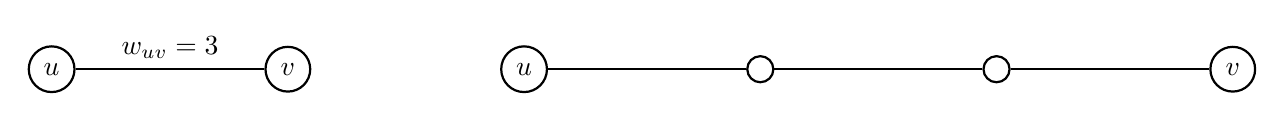
\begin{tikzpicture}[node distance={30mm}, thick, main/.style = {draw, circle}]
      \node[main] (1) {$u$};
      \node[main] (2) [right of=1] {$v$};

      \node[main] (3) [right of=2] {$u$}; 
      \node[main] (4) [right of=3] {};
      \node[main] (5) [right of=4] {};
      \node[main] (6) [right of=5] {$v$}; 

      \draw (1) -- (2) node[midway, above] {$w_{uv} = 3$};

      \draw (3) -- (4);
      \draw (4) -- (5);
      \draw (5) -- (6);
    \end{tikzpicture}
  \end{center}

  Let's look at an alternative...

  \subsubsection{Dijkstra's Algorithm}

  Let $G$ be our graph, and $s$ be our starting vertex. Dijkstra's algorithm finds
  the minimum distance of every node to $s$.

  \begin{lstlisting}
Dijkstra($G$, $s$):
  # we break our graph $G$ up into its
  # edge set $E$ and vertex set $V$
  let $E$, $V$ = $G$

  # d[$v$] represents the distance of vertex $v$
  # from $s$, so the distance from $s$ to $s$ is 0
  let $d[s]$ = 0

  # this is the parent of $s$
  let $\pr[s] = \emptyset$

  # we initialize all vertices that aren't $s$ as
  # being infinitely far, since we don't know how
  # far they are
  for all $v \in V \setminus \{s\}$:
    $d[v]$ = $\infty$

  mark all vertices as unexplored

  while $\exists$ unexplored vertices:
    let $u$ be the unexplored vertex with smallest $d[u]$

    for each neighbor $v$ of $u$:
      let $w_{uv} \in E$ be the weight of the edge connecting $u$ to $v$

      if $d[u]$ + $w_{uv}$ < $d[v]$:
        # this is a better upper bound
        $d[v]$ = $d[u]$ + $w_{uv}$
        $\pr[v]$ = $u$
      end if
    end for

    marked $u$ as explored
  end while
  \end{lstlisting}

  \subsubsection{Proof of Dijkstra's algorithm}

  \note {
    Dijkstra's algorithm requires all edge weights to be {\bf positive}.
  }

  \Lemma {
    When a vertex $v$ is explored, $d[v]$ is the distance from $s$ to $v$.
  }
  {
    {\it By induction on the number of explored vertices}.

    By induction on the number of explored vertices. Clearly, it holds when only
    $s$ is explored.

    Suppose that the lemma holds when there are $k$ explored vertices. Let $v$
    be the $(k + 1)^{\text{st}}$ explored vertex, and let $\pr[v] = u$.

    Suppose for the sake of contradiction, that the shortest path from $s$ to
    $v$ does not go through $u$. Instead, let $x \ne u$ be the last explored
    vertex on the shortest path, and let $y$ be its unexplored neighbor on this
    path.

    Note that $y \ne v$, otherwise the algorithm would choose $u = x$.

    \begin{align*}
      \text{dist}(s, v) <&d[v] \\
                      \le&d[y]          &\text{since we chose to add $v$ before $y$} \\
                      =&\text{length of a path from $s$ to $y$ found} & \\
                    \le&\text{dist}(s, v) &\text{since, by contradiction, $y$ is on the shorted path from $s$ to $v$} \end{align*}

    But this is a contradiction, so the shorted path from $s$ to $v$ must go through
    $u$, and it must be the case that

    \[
      \text{dist}(s, v) = d[u] + w_{uv} = d[v]
    \]
  }

  % {\bf Picture}

  % \TODO{} this picture means nothing, either finish it or remove it.
  %
  % \begin{center}
  %   \begin{tikzpicture}[node distance={15mm}, thick, main/.style = {draw, circle}]
  %     \draw[gray] (0,0) ellipse (2cm and 1cm);
  %
  %     \node[main] (1) {$s$};
  %     \node[main] (2) [right of=1] {$u$};
  %     % \node[main] (2) [right of=1] {$v$};
  %     %
  %     % \node[main] (3) [right of=2] {$u$}; 
  %     % \node[main] (4) [right of=3] {};
  %     % \node[main] (5) [right of=4] {$v$}; 
  %     %
  %     % \draw (1) -- (2);
  %     % \draw (3) -- (4);
  %     % \draw (4) -- (5);
  %   \end{tikzpicture}
  % \end{center}

  \subsubsection{Running Time}

  The running time of Dijkstra's algorithm is very similar to the other algorithms
  we've seen so far. It can be shown that the running time is $\O(m + n)$.

  \newpage

  \subsection{Minimum Spanning Trees}

  We're interested in finding a spanning tree for a given graph. But now we don't
  want to find the distance between any two vertices, but we want to {\it minimize
  the total minimum weight of the edges in the tree}.

  These weights just have to be real numbers, they don't have to be positive.

  % \TODO{} verify the above.

  If we want to have a communications networks between nodes, this might be
  applicable. The edge weight might represent the cost of building that cable, or
  the distance, or anything else that you want.

  {\bf Example}

  \begin{center}
    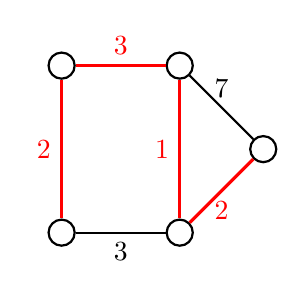
\begin{tikzpicture}[node distance={15mm}, thick, main/.style = {draw, circle}] 
      \node[main] (1) {};
      \node[main] (2) [right of=1] {};
      \node[main] (5) [below right of=2] {}; 
      \node[main] (4) [below left of=5] {};
      \node[main] (3) [left of=4] {}; 

      \draw[red, very thick] (1) -- node[above] {3} (2) ;
      \draw[red, very thick] (2) -- node[left] {1} (4);
      \draw[red, very thick] (1) -- node[left] {2} (3);
      \draw (3) -- node[below] {3} (4);
      \draw[red, very thick] (4) -- node[below] {2} (5);
      \draw (2) -- node[above] {7} (5);
    \end{tikzpicture}
  \end{center}

  In this graph, the red edges form a minimum spanning tree. Note that there can
  be multiple minimum spanning trees from a single graph.

  {\bf Question}

  How do we know which edges to add to our tree?

  \Definition {Cut} {
    A {\bf Cut} is a {\it bipartition} (a partition into two sets) of the
    vertices, $V = A \cup B$ with $A \cap B = \emptyset$.

    A cut is {\bf non-trivial} if both $A$ and $B$ are non-empty.

    An edge {\bf crosses} the cut if it has one end in $A$ and one end in $B$.
  }

  \Lemma {
    Assume that all edge weights are distinct. Let $(A, B)$ be a non-trivial
    cut, and let $e$ be the minimum weight edge crossing this cut. Then, any
    minimum spanning tree must contain $e$.

    We will prove this using an {\it exchange argument} (we will use this again
    a lot for greedy algorithms as well as scheduling algorithms.)
  }
  {
    Let $T'$ be a spanning tree that does {\it not} contain $e = \{u, v\}$. Since
    $T'$ is spanning, there is {\it a unique, simple} path from $u$ to $v$.

    Since $e$ crosses the cut, there must be {\it at least} one edge along the path
    from $u$ to $v$ that crosses the cut (if there is more than one, that's fine),
    call this edge $e'$.

    {
      \it At this point, our graph is partitioned into two parts, $A$, and $B$.
      $e$ is not in the MST, but $e'$ is. Both $e$ and $e'$ cross from $A$ to
      $B$. What we're gonna do here is swap edge $e$ and $e'$
    }

    Construct a new spanning tree $T$ from $T'$ by deleting $e'$ and adding $e$.

    This is still a tree since the number of vertices is $n$, the number of edges is
    $n - 1$, and the graph is fully connected. Therefore it cannot contain any
    cycles.

    Since the weight of $e$ is less than the weight of $e'$, this change lowers the
    total edge weight of the spanning tree.
  }

  Using this lemma, let's now look at various algorithms for finding MSTs.

  \subsubsection{Kruskal's Algorithm}

  {\bf Main Idea}: {\it Add the lowest cost edge that doesn't create a cycle.}

  {\bf Process}

  \begin{enumerate}
    \item Sort all edges in $G$ by weight, lowest to highest.
    \item Iterate through sorted edges, add it to the Minimum Spanning Tree {\bf
      if} it doesn't create a cycle.
  \end{enumerate}

  % \begin{lstlisting}
  % Kruskal($G$):
  %   Add the lowest cost edge that doesn't create a cycle.
  % \end{lstlisting}

  {\bf Correctness}

  \Theorem {
    Kruskal's Algorithm always outputs a Minimum Spanning Tree.
  }
  {
    Suppose that the algorithm adds the edge $e = \{u, v\}$ to the forest $F$.
    Consider the cut induced by the component of $u$ in $F$.

    {
      \it One side of this cut is everything connected to $u$, and the other side
      is everything connected to $v$.
    }

    Clearly, $e$ crosses this cut and, by definition, it is the minimum weight
    edge with that property. So by the Lemma, any MST must include $e$.

    {
      \it Note that this works at any stage along the algorithm. So the only thing
      that we need now is to show that the output is a spanning tree, and if it
      is, it will automatically be minimal.
    }

    Note also that it clearly does not create a cycle. If the graph were not
    connected, then it could add some edge without creating a cycle, so the output
    must be a tree.
  }

  Let's now look at another way to produce Minimum Spanning Trees: Prim's algorithm.

  {\bf Running Time}

  For Kruskal's algorithm, a {\it union-find} data structure is helpful. If done
  properly, the running time can be $\O(m \log n)$.

  \subsubsection{Prim's Algorithm}

  {\bf Main Idea}: {\it Chose a root to grow a Spanning Tree from.}

  {\bf Process}

  \begin{enumerate}
    \item Chose a starting vertex. This is the root of the Minimum Spanning Tree.
    \item Look at the set of all edges connected to the nodes in our Minimum
      Spanning Tree.

    \item From these edges, only consider the ones that point to
      vertices that are {\bf not} already in our MST. As you go, mark vertices
      as explored.

    \item Of these edges, add the one with lowest weight.
      %
      % Repeatedly add the non-tree vertex with the lowest connection cost.
      %
      % Look at every vertex in your spanning tree thus far, and find the vertex
      % whose edge has the lowest weight, this is the vertex that you add.
  \end{enumerate}

  Repeat this process until all vertices are explored.

  {\bf Correctness}

  \Theorem {
    Prim's algorithm outputs a MST.
  }
  {
    Suppose the algorithm adds edge $e = \{u, v\}$ to the forest $F$. Consider the
    cut induced by component of the root (from which the algorithm builds the
    tree).

    Clearly $e$ crosses this cut and, by definition, it is the minimum weight edge
    with that property.

    So by the Lemma, every MST contains $e$ and so clearly, Prim's algorithm
    outputs a Spanning Tree.
  }

  \note {
    Both of these algorithms pertain to undirected graphs. The graphs {\it could}
    have cycles.

    Both of these algorithms are also {\it greedy}.
  }

  Implementing these algorithms efficiently require choosing good data structures.

  {\bf Running Time}

  For Prim's algorithm, you often want a {\it priority queue} to store edges of
  the graph. If done properly, a running time of $\O(m\log n)$ is possible.

  \subsection{Scheduling}

  % \note {
  %   On Feb. 28 Class will be in ESJ 2204.
  % }
  %
  % \note {
  %   Midterm is on march 9th. There is only one exam
  % }

  {\it You have to be very careful in how you're greedy to get an algorithm that
  works.}

  This is another set of greedy algorithms.

  \note {
    {\bf Midterm}

    Divide and conquer might be the last topic before the midterm.
  }

  We'll look at 3 different examples of scheduling algorithms. 

  \subsubsection{Interval Scheduling}

  {\it Which classes should be in which rooms.}

  For now, suppose that we have one room, and a bunch of requests for it. How many
  classes can you schedule.

  Suppose that you are given $n$ request, which come with starting times $s_i$ and
  finishing times $f_i$ for an $1 \le i \le n$. Note that $f_i \le s_i$.

  We cannot hold two classes at the same time. A subset of requests is {\bf
  compatible} if no two of the intervals overlap in time.

  {\bf Goal}

  Our goal is to hold as many classes as possible, and the duration of a class
  does not matter to us (a 10 minute class is just as valuable as a 90 minute
  class).

  Let's look at an example

  % {\bf Example}
  %
  % \TODO{} Draw schedule picture from Feb 23
  %
  % In this example, $2, 5, 6$ satisfies the problem but $1, 5, 6$ also work.

  \note {
    In general, {\it solutions may not be unique, but we only need to find one}.
  }

  How do we write such an algorithm? We want to find the {\it best} solution.
  What's a natural way to be greedy here? In what order should we look at the
  intervals? This is going to matter a lot.

  {\sc Idea 1}.

  What if we try to think about the shortest activities first? This is actually
  sub-optimal, If you have a really long task and another really long task, with a
  really short task right between the two long tasks, then you're not doing as
  best as you could.

  {\sc Idea 2}.

  What if we try to find the activity with the minimum number of conflicts first?
  This is very natural, but not optimal. You can give a counter example to this,
  even if it's not easy.

  {\sc Idea 3}.

  What if we sort activities by starting time? This is sub-optimal. What if the
  earliest starting interval finishes last? What if it knocks out 10 other
  intervals that could have been better?

  {\sc Idea 4}.

  What if we consider each interval on its own, and then find the earliest
  finishing one? This is optimal! (among potentially many other solutions).

  Find the earliest activity first, 

  {\bf Pseudocode}

  \begin{lstlisting}
GreedyIntervalSchedule($s$, $f$):
  sort tasks by increasing order of finishing times.
  # note that you will need to sort $s$ in the same way as $f$

  let $A = \emptyset$
  let $f_\text{prev} = -\infty$

  for i in 1 to n:
    # this interval starts after the previous interval finishes it doesn't
    # conflict, so add it
    if $s_i > f_\text{prev}$:
      add task $i$ to $A$
      set $f_\text{prev} = f_i$
    end
  end
end
  \end{lstlisting}

  This is clearly $\O(n \log n)$ for sorting, since everything else is constant
  time.



  {\bf Proof of Correctness}

  Why does this work?

  \begin{enumerate}
    \item There are no conflicts, since we only schedule a task that starts after
      the current one ends.

    \item We'll show that the number of tasks is maximal by an {\bf exchange
      argument}. We can also show that this algorithm stays ahead (see book.)
  \end{enumerate}

  \Theorem {
    \texttt{GreedyIntervalSchedule} outputs an optimal schedule.
  }
  {
    Let $G = (g_1, g_2, ..., g_k)$ be the greedy schedule, with indices
    representing tasks in order of increasing finish time.

    Let $B = (b_1, ..., b_l)$ be an optimal schedule, with $l \ge k$.

    % \btw { Want to conclude that $l = k$ }

    Let $j$ be the first index where the schedules differ

    \[
      g_1 = b_1, \dots, g_j = b_j, g_{j + 1} \ne b_{j + 1} \dots
    \]

    Now switch $B' = (g_1, \dots, g_{j - 1}, g_j, b_{j + 1}, \dots, b_l)$. By the
    greedy choice, we know that the finishing time of $g_j \le b_j$, so there are
    no conflicts, and it is just as long: $l$ intervals.

    \btw{
      This is the essence of the exchange argument. We started with a
      perfect schedule and demonstrated that we could exchange it inductively and
      retain an optimal schedule.
    }

    Repeating this process, we get a schedule

    \[
      (g_1, \dots, g_k, b_{k + 1}, \dots, b_l)
    \]

    If $l > k$, then $b_{k + 1}$ is the index of some interval that the greedy
    algorithm could have scheduled, but it didn't which is a contradiction, so $l$
    must equal $k$.

    Therefore the greedy algorithm is optimal.
  }

  \note {
    Solutions to the greedy algorithm may not be unique! It's possible to use
    this exchange argument to produce different optimal schedules.
  }

  \subsubsection{Interval Partitioning}

  Suppose that we must schedule all intervals, given again by starting and
  finishing times, while minimizing the number of resources used (in this case,
  the number of classrooms, where each classroom is the same size).

  What is the minimum number of classes necessary to accommodate all schedules?

  % {\bf Example}
  %
  % \TODO{} Draw picture
  %
  % Here, 3 intervals suffice. It's impossible to get 2 however, the reason for this
  % is that there are 3 simultaneous classes at the end of the day.
  %
  % You can use this {\it dashed line} to find bounds on the problem more easily.
  %
  % Let's call this lower bound the depth.

  \Definition {Interval Depth} {
    The {\bf depth} of a set of intervals is the maximum 

    \[
      \text{max}_t \Big\{i \in \{ 1, \dots, n\} : t \in [s_i, f_i] \Big\}
    \]

    In other words, for every $1 \le i \le n$, this is the maximum number of
    overlapping intervals.

    Which is the largest number of overlapping subsets.
  }

  \note {
    The depth is {\it always} the optimal solution. It's possible to always reach
    it.
  }

  {\bf Greedy Approach}

  Scan through intervals in increasing order of start time. Assign each to any
  available resource from 

  \[
    \{1, \dots, \text{depth}\}
  \]

  \Theorem {
    This algorithm assigns a color from $\{1, \dots, \text{depth}\}$ to every
    interval and no two overlapping intervals have the same color.
  }
  {
    When we assign a color, it is, by definition of the algorithm, different from
    the colors of all the overlapping intervals that are already scheduled. So
    because of that, we never assign the same color to overlapping intervals.

    Suppose that, when we are considering the $i^\text{th}$ interval, it overlaps
    $t$ previous intervals. So, in the input, there exists $t + 1$ overlapping
    intervals. So the depth is at least $t + 1$, but conversely, that tells us
    that $t$ is at most $\text{depth} - 1$. So there is always a color available.
  }

  The pseudocode for this algorithm was not shown in class, but it was mentioned
  that optimal runtime was $\O(n \log n)$.



  \subsection{Schedule to Minimize Lateness}

  We have a number of schedules, and only one room. We have to schedule all of
  them. Each schedule is defined by a duration and a deadline. There's some
  time by which we would like to finish the request. There is not specified
  starting time. Let's formalize this.

  {\bf Setup}: We are given tasks with duration $t_i$, and deadline $d_i$.

  It might not be possible to always satisfy each deadline, but we want to
  minimize lateness.

  If we schedule job $i$ from the interval $[s_i, f_i]$ with $f_i = s_i + t_i$.
  We say that the lateness of job $i$, called $l_i$ is defined as follows

  \[
    l_i = \max(0, f_i - d_i)
  \]

  In other words, it's either $0$ if the job finishes before its deadline, or
  some positive real number otherwise.

  Concretely, our goal is to schedule all jobs without overlaps, while
  minimizing the worst case lateness defined as $\max_i(l_i)$.

  \note {
    Here we are not trying to minimize {\it total} lateness, just the {\it
    worst} lateness.
  }

  Let's look at an example

  \Example {
    Let's look at the following jobs.

    $J = \{(t_1 = 1, d_1 = 2), (t_2 = 3, d_2 = 1)\}$
  }
  {
    It's always in our best interest to have a job running at any time if we are
    free.

    From this job list, we can chose to run the jobs in the following order

    $1, 2$, for which the lateness would be $l_1 = 0, l_2 = 3$
    or $2, 1$ for which the lateness would be $l_1 = 2, l_2 = 2$

    Since the worst case lateness in the second ordering is only $2$, the second
    ordering is better.
  }

  We'll solve this problem using a greedy strategy. Let's first take a look at
  some natural approaches we could take for this problem.

  {\bf Approaches}

  \begin{enumerate}
    \item Go in order of increasing deadline. Start with the job with the
      earliest deadline $d_i$. This {\it will} actually prove to be optimal!

    \item Go in order of shortest duration $t_i$ first. If you have some jobs
      you could get done quickly, you might want to get those out of the way
      first. Unfortunately this is can be shown not to be optimal

      Consider the following jobs

      $J = \{(t_1 = 0, d_1 = 100), (t_2 = 10, d_1 = 10)\}$

      Then we would do $t_1$ first, and then $t_2$, which would yield a max
      lateness of $10$, whereas doing $t_2$ and then $t_1$ would yield $0$
      lateness.

    \item Go in order of ``slack": How much extra time remains after a job
      finishes? Jobs that give you the highest amount of slack sound really good
      to do first, surely. It can be shown that this is also not optimal.
  \end{enumerate}

  What this illustrates is that the {\it way} in which we are greedy about a
  problem matters a lot. There are many things that sound sensible to do, but
  actually lead to sub-optimal solutions. It's worth taking the time to try to
  figure out what to be greedy about.

  We'll now look into the first approach, and prove that it is optimal by an
  exchange argument.

  To help understand why this is optimal, we'll first introduce the concept of
  an {\it inversion}.

  \definition {
    A schedule has an {\bf Inversion} if job $i$ comes before job $j$, but it is
    also the case that $d_i > d_j$.
  }

  Recall that our approach is to sort by increasing deadline. If in our
  ordering we have two jobs whose deadlines behave in the way defined above, it
  is what we call an inversion.

  In our optimal schedule, we want no inversion.

  \Lemma {
    All schedules with no inversions (there can be more than one!) and no idle
    time (this is assumed, just remove the idle time otherwise) have the same max lateness.
  }
  {
    \btw {
      How can this happen? Well let's first ask how we can have two different
      schedules with no inversions. This can only be the case if two jobs have
      the same deadline! After all if they did not, they would be in some order
      according to our greedy strategy.
    }

    The only flexibility in such a schedule is in the order of jobs with the
    same deadline. Moreover, any such jobs would be ordered consecutively. The
    finishing time of the last of these jobs doesn't depend on the ordering.
  }

  \Lemma {
    There is an optimal schedule with no inversions (and no idle time).
  }
  {
    We'll prove this using an exchange argument.

    {\it Goal}. We'll suppose that we have an optimal schedule which {\it has}
    inversions, then we'll show that we can exchange out such inversions without
    losing quality.

    If there is an inversion, then there must be jobs $i, j$ which are adjacent
    (with $i$ before $j$ WLOG) with $d_i < d_j$. In other words, if we have an
    inversion (adjacent or not), then we {\it must} have an adjacent inversion.
    You can reason about this by contradiction, but the argument is a sort of
    intermediate value theorem.

    Now we'll swap the two jobs and see what happens to the lateness. This
    decreases the total number of inversions. The claim now is that the max
    lateness is no worse.

    Swapping $i$ and $j$ gives a schedule with one less inversion, and we claim
    that there is no worse lateness.

    Why is the lateness no worse? Well suppose we have the following scenario.
    Job $i$ comes before job $j$, and $d_j < d_i$ come before the start of job
    $i$. Then, it's clear that that the max lateness is driven by $f_j - d_j$.

    Swapping $i$ and $j$, the lateness is

    \[
      \max(f_j - d_i, (s_i + f_j - s_j) - d_j) = \max(f_j - d_i, f_j - d_j - (s_j - s_i))
    \]

    but $s_j - s_i \ge 0$. Clearly the lateness we get by doing this is going to
    be $l \le f_j - d_j$ since $d_i > d_j$ and $s_j - s_i \ge 0$.

    Repeating this, we eventually get a schedule with no inversions and no worse
    lateness.
  }





  \newpage

  \sidenote {
    Exam one week from today. No calculator needed, can bring notes.
    For proofs, you don't need to write five pages. See solutions for examples.

    Format of the exam: similar to practice problems. Suggestion: make a question
    out of three short answer questions. Longer questions are problems are gonna be
    like homework questions. Proving mathematical fact, run algorithm that you know
    on some data, etc...

    Look at practice problems!

    Assignment 2 should be graded a bit before exam 2
  }

  \section{Divide and Conquer}
  {\it This is the last topic on the exam}

  {\bf Main Idea}: Divide into sub problems, usually 2, but not necessarily. We'
  solve the sub problems recursively, and merge the solutions, maybe with some
  additional work, to solve the overall problem.

  \subsection{Merge Sort}

  To sort a list of length $n$
  \begin{itemize}
    \item Divide the list in half
    \item Sort each half, recursively, using this exact procedure.
    \item Merge the two sorted lists. You can do this in linear time! This is what makes
      Merge Sort great.
  \end{itemize}

  \subsubsection{Running Time}
  
  Let $T(n)$ be the running time on instances of length $n$. Let's write a
  recurrence equation for Merge Sort.

  \[
    T(n) = 2 \cdot T(n / 2) + \O(n), \, \, T(1) = \O(1)
  \]

  \note {
    The first part of the recurrence represents the work necessary to complete
    Merge Sort on a list of length $n / 2$, which there are $2$ of. The second
    part represents the work necessary to merge the two lists together.
  }

  Solving this recurrence, we get that $T(n) = \O(n \log n)$.

  {\bf Question}: What if $n$ isn't even?

  It's important to note what we're doing here. The recurrence equation we
  described above represents an {\it upper bound} for the running time of Merge
  Sort. If the two lists aren't the same size, then the time needed to sort each
  will just be bounded above by the time necessary to sort twice the larger one,
  and merge twice the larger one. If the lists aren't the same size, the time
  can only be better.

  % Last time we talked about Merge Sort, how to give an $\O(n \log n)$ time. We saw
  % the general structure of how it worked. Merge can be done in linear time.
  %
  % {\bf Merge Sort Recurrence}
  % \begin{align*}
  %   T(n) =&2 \cdot T(n / 2) + \O(n) \\
  %        =&\O(n \log n)
  % \end{align*}

  Not {\it all} divide and conquer algorithms are $\O(n \log n)$. Recall Karatsuba
  multiplication, which is also divide and conquer. This algorithm was still
  $\O(n^2)$, but just had a better constant term.

  \subsubsection{Pseudocode}

  \begin{lstlisting}
MergeSort($L$):
  # get the size of the list
  let $n$ = $|L|$

  # the list is length $1$ or less
  if $n \le 1$:
    return $L$

  # get the lower midpoint of the list
  let $m$ = $\lfloor n / 2 \rfloor$

  # get the sorted left and right sublists
  let $l$ = MergeSort($L$[$0$ to $m$])
  let $r$ = MergeSort($L$[$m$ to $n$])

  return Merge($l$, $r$)
end
  \end{lstlisting}

  Where $L$ is our list, and \texttt{Merge} is defined as

  \begin{lstlisting}
Merge($l$, $r$):
  let $S$ = []
  let $i = j = 0$

  while $i < |l|$ and $j < |r|$:
    if $l$[$i$] $\le$ $r$[$j$]:
      $S$.push($l$[$i$])
      $i$++
    else:
      $S$.push($r$[$j$])
      $j$++

  # in case the two lists aren't the same size
  # only one of these loops will be entered
  while $i < |l|$:
      $S$.push($l$[$i$])
      $i$++
  while $j < |r|$:
      $S$.push($r$[$j$])
      $j$++

  return $S$
end
  \end{lstlisting}

  \subsection{Closest Points}

  Suppose we have $n$ points in in the plane, and we want to find the two closest
  points.

  \subsubsection{One Dimensional Case}
  We explored a simpler version of this problem in one dimension. Suppose that
  instead the points are in a line, how do you find the closest two? If the points
  are given in arbitrary order you have to sort, and then go through them from
  left to right.

  In one dimension, you sort by $x$ coordinate but you can't just do that in 2
  dimensions. Still, we can sort the points in {\it some} way that can help. Once
  the points are sorted, we can work with them in some other way.

  Let's define the problem better.

  \subsubsection{Two Dimensional Case}

  Suppose that we are given $n$ points in a plane, in no order whatsoever, and
  no two points overlap.

  % We want to divide the points into halves.

  {\bf Main Idea}: We could recursively subdivide the points into left and right
  based on the {\it median} $x$ coordinate of the points, and divide left and
  right. Then we solve the closest pair problem on each half. 

  \note {
  The closest pair of points {\it could} be across the line, our algorithm needs
  to consider this. In other words we want to check whether there is a closer
  pair with one on the left and one on the right.
  }

  As we recurse, we maintain lists of the points in our subsets sorted by $x$ and
  $y$ coordinate. We store this is in 2 separate lists by just sorting the indices
  on $x$ and $y$.

  Let's define some notation.

  Suppose that the input points $P = \{p_1, \dots, p_n\}$ where $p_i = (x_i,
  y_i)$. 
  \begin{itemize}
    \item Let $Q$ be the points in $P$ with the first $\lceil n / 2 \rceil$ $x$
      coordinates, and let $R$ be the points in $P$ with the last $\lfloor n / 2
      \rfloor$ $x$ coordinates, in other words: the remaining points.

    \item We recursively find the closest points in $Q$, call them $q_0^*,
      q_1^*$, and $R$, call then $r_0^*, r_1^*$.

    \item Let $\delta$ be the minimum between $\text{dist}(q_0^*, q_1^*)$, and
      $\text{dist}(r_0^*, r_1^*)$.

      In other words, $\delta$ represents the distance between the two closest
      points either on the left side, or the right side of the line.

    \item Let $x^*$ be the largest $x$ coordinate of a point in $Q$.

      In other words, $x^*$ is the point closest to the line on the side of $Q$.
      In fact, the line crosses over the point $x^*$.

    \item Let $L$ be the line $x = x^*$.
  \end{itemize}

  \btw {
    So what we're doing here is that we look at every point in $Q$ and $R$, and
    find the closest two and we define $\delta$ based on this distance. 

    But what if the closest two points are actually between $Q$ and $R$? Let's
    explore this possibility in the next lemma.
  }

  {\bf Lemma}. If there is a $q \in Q$ and $r \in R$ with $\text{dist}(q, r) <
  \delta$, then both $q$ and $r$ are within $\delta$ of $L$.

  What this tells us is that we can restrict attention to a strip of length
  $2\delta$ centered on $L$. This is nice, but keep in mind that all points could
  be in that strip.

  \Lemma {
    If two points in $S$ have distance less than $\delta$, then they're within
    15 positions of each other in the list of points sorted by $y$ coordinate.

    {\it Why 15? Who knows! Its just some weird constant not explained in class.
    Just believe in the Lemma}.
  }
  {
    Divide $S$ into squares of side length $\frac{\delta}{2}$.

    {\bf Claim}. No two points can be in the same square. If they were, then
    $\delta$ would be smaller by definition of $\delta$.

    Suppose that two points in $S$ are 16 or more positions apart in the list sorted
    by $y$ coordinate. Then they have to differ by {\it at least} 3 rows of boxes,
    so they have distance at least

    \[
      3 \cdot \frac{\delta}{2} > \delta
    \]

    In other words, {\it because} their distance is greater than $\delta$, then
    there {\it must} be {\it at least} 3 empty boxes between them.
  }


  \subsubsection{Running Time}

  The cost of finding the two closest points is $T(n / 2)$. Since there are two
  sides we have cost

  $T(n) = 2T(n / 2) + \O(n)$

  Where $\O(n)$ is the cost of merging the two sides, and since the lists are
  sorted, the cost of this is linear.

  \subsection{Fast Fourier Transform}

  {\it This is one of the best algorithms of all time}

  This is a great way to multiply polynomials, but it's also used in signal
  processing, and many other fields. For now, we'll restrict our problem to the
  following.

  Suppose that we are given a polynomial $a(x), b(x)$ of degree $n - 1$

  \[
    a(x) = a_0 + a_1x + \cdots + a_{n - 1}x^{n - 1}
  \]

  and

  \[
    b(x) = b_0 + b_1x + \cdots + b_{n - 1}x^{n - 1}
  \]

  Suppose now that $c(x)$ is defined as $c(x) = a(x) \cdot b(x)$. We'll see how to
  multiply this next time.

  \sidenote {
    Everything about Divide and Conquer is on the exam. Dynamic Programming is
    not.
  }

  \sidenote {
    The Fast Fourier transform uses some linear algebra. You aren't really
    responsible for this part on the exam, just know how exactly the task is
    divided.
  }

  We've been talking about Divide and Conquer algorithms, we looked at the
  closest points problem and we started talking about polynomial multiplication,
  which will motivate the Fast Fourier Transform.
  
  Recall polynomial multiplication, we can suppose that the coefficients are in
  $\R$, or even $\C$ if we wanted to.

  \[
    a(x) = a_0 + a_1x + \cdots + a_{n - 1}x^{n - 1}
  \]

  and

  \[
    b(x) = b_0 + b_1x + \cdots + b_{n - 1}x^{n - 1}
  \]

  Suppose now that $c(x)$ is defined as $c(x) = a(x) b(x)$.

  What is $c(x)$?

  \begin{align*}
    c(x) =&a(x) \cdot b(b) \\
         =&\left(\sum_{j = 0}^{n - 1}a_j \cdot x^j\right)\left(\sum_{j = 0}^{n - 1}b_j \cdot x^j\right) \\
         =&\sum_{j,k = 0}^{n - 1} a_j \cdot b_k \cdot x^{j + k} & \text{Can combine the sums} \\
         =&\sum_{l = 0}^{2n - 2} \left( \sum_{j = 0}^{l} a_j \cdot b_{l - j} \right) x^l & \text{$l = j + k$, both go up to $n - 1$} \\
         =&\sum_{l = 0}^{2n - 2} c_l x^l & \text{Define $c_l = \sum_{j = 0}^{l} a_j \cdot b_{l - j}$} \\
  \end{align*}

  \note {
    If both $a(x)$ and $b(x)$ are both degree $n - 1$, $c(x) = a(x)b(x)$ will be of degree $l = 2n - 2$.

    More generally, if $a(x)$ is degree $n$ and $b(x)$ is degree $m$, then $c(x) = a(x)b(x)$ is
    degree $nm$.
  }

  What we can gather from this is that, if we were to compute this manually, it
  would be $\O(n^2)$. However using Divide and Conquer can really help us here.

  {\bf Main Idea}: Use polynomial Interpolation.

  A degree $d$ polynomial can be uniquely specified by its values at any $d + 1$
  points. Not necessarily its roots, but {\it any} points on that polynomial

  \note {
    If you plot $2$ two points, there's a unique line that goes through them. If
    you plot $3$ points, there is a unique parabola that goes through them. If
    you plot $4$ points, there is a unique cubic, etc...

    More generally, given $n$ points, there is a unique polynomial of degree $n
    + 1$ that goes through it.
  }

  This is a linear amount of work! If we can somehow divide and conquer on this,
  we have an algorithm. Let's devise a strategy.

  \subsubsection{Strategy}

  \begin{enumerate}
    \item Evaluate the polynomials $a$ and $b$ on $2n - 1$ points. Somehow, we
      have to do this in close to linear time.

      {\it We'll have to pick these points carefully!}

      \note {
        You need $2n - 1$ points because $c(x)$ is degree $2n - 2$, and
        you need one more point to identify $c$ from that, from the previous
        note.
      }

    \item Evaluate $c(x)$ on those points.

    \item Reconstruct the coefficients of $c(x)$ from the points.

  \end{enumerate}

  \btw {
    We'll see that (1) and (3) are actually the same problems in reverse!
  }

  Now let's dive deeper into each step.

  \subsubsection{Process}

  \begin{enumerate}
    \item {\it Evaluate $a$, $b$ on $2n - 1$ points}
       
      First we compute $\O(n)$ points on $a$ and $b$, each of which takes $O(n)$ time to
      evaluate individually, since both polynomials have $\O(n)$ terms. 

      Consider evaluating a polynomial of degree $d - 1$ at $d$ points $x_0,
      x_1, \dots, x_{d - 1}$

      \[
        a(x_j) = a_0 + a_1 x_j + \cdots + a_{d - 1} x_j^{d - 1}
      \]

      Assume $d$ is even for simplicity. Define

      \begin{align*}
        a_\text{even}(x) =&a_0 + a_2 x + a_4 x^2 + \cdots + a_{d - 2} x^{(d / 2) - 1} \\
        a_\text{odd}(x) =&a_1 + a_3 x + a_5 x^2 + \cdots + a_{d - 1} x^{(d / 2) - 1}
      \end{align*}

      Then we have

      \[
        a(x) = a_\text{even}(x^2) + x \cdot a_\text{odd}(x^2)
      \]

      Each of these polynomials are half the size.

      {\bf Picking points carefully}

      % \TODO{} Cleanup:
      Consider the points $1, -1, i, -i$. Squaring these points, we get $1, 1,
      -1, -1$. Squaring again, we get $1, 1, 1, 1$.

      The natural choice for these points are the $d^\text{th}$ {\bf roots of
      unity}!

      \[
        x_j = \omega_d^j
      \]

      Where $\omega_d = e^{\frac{2 \pi i}{d}}$.

      \note {
        If we square $d^\text{th}$ roots of unity, we get half as many points.

        Let's see this in action.

        $x_j = \omega_d^{j}$. Squaring, we get

        \begin{align*}
          x_j^2 =&\omega_d^{2j} \\
          =&e^{\frac{2 \pi i}{d} (2j)} \\
          =&e^{\frac{2 \pi i}{d} (2j) \Mod d} \\
          % =&e^{\frac{4 \pi i}{d} j \Mod d} \\
          =&\omega_d^{2j \Mod d} \\
          =&x_{2j \Mod d}
        \end{align*}

        % \TODO{} cleanup and explain better
      }

      If $T(d)$ is the cost of evaluating $a(x)$ at $x_j$ for $j \in \{0, 1,
      \dots, d - 1\}$, then we have

      \begin{align*}
        T(d) =&2T(d / 2) + \O(d) \\
             =&\O(d \log d)
      \end{align*}

      Is the cost of evaluating $a(x)$ on $d$ points.

      \note {
        If our polynomial isn't perfectly even, we can pad it out to make it a
        power of $2$. It doesn't really matter.
      }

    \item {\it Evaluate $c(x)$}

      % \TODO{} what?? did we skip this??

    \item {\it Reconstruct $c(x)$}

      Consider how the coefficients of a polynomial relate to its evaluations at
      $\omega_d^0, \omega_d^1, \dots, \omega_d^{d - 1}$.

      So we have

      \begin{align*}
        a(x) =&a_0 + a_1 x a_2 x^2 + \cdots + a_{d - 1} x^{d - 1} \\
        =&\begin{bmatrix}
          1 & x & x^2 & \cdots & x^{d - 1}
        \end{bmatrix}
        \begin{bmatrix}
          a_0 \\
          a_1 \\
          \vdots \\
          a_{d - 1}
        \end{bmatrix}
      \end{align*}

      So we have

      \[
        \underbrace {
          \begin{bmatrix}
            a(\omega_d^0) \\
            a(\omega_d^1) \\
            a(\omega_d^2) \\
            \vdots \\
            a(\omega_d^{d - 1})
          \end{bmatrix}
        }_{x}
        =
        \underbrace{
          \begin{bmatrix}
            1 & \omega_d^0 & \left( \omega_d^0 \right)^2 & \cdots & \left( \omega_d^0 \right)^{d - 1} \\
            1 & \omega_d^1 & \left( \omega_d^1 \right)^2 & \cdots & \left( \omega_d^1 \right)^{d - 1} \\
            1 & \omega_d^2 & \left( \omega_d^2 \right)^2 & \cdots & \left( \omega_d^2 \right)^{d - 1} \\
            \vdots & \vdots & \vdots & \ddots & \vdots \\
            1 & \omega_d^{d - 1} & \left( \omega_d^{d - 1} \right)^2 & \cdots & \left( \omega_d^{d - 1} \right)^{d - 1} \\
          \end{bmatrix}
        }_{F}
        \underbrace{
          \begin{bmatrix}
            a_0 \\
            a_1 \\
            a_2 \\
            \vdots \\
            a_{d - 1}
          \end{bmatrix}
        }_{y}
      \]

      This is the discrete Fourier transform! As it turns out, $F$ is a unitary
      matrix, meaning that its inverse is easy to compute.

      We have (x = a omega vector). We want (y = ai vector). 

      We have that

      \[
        x = \frac{1}{\sqrt{d}} F y
      \]

      So

      \[
        y = \sqrt{y} F^{-1} x
      \]

      which reconstructs $c$.

      Since $F$ is unitary, $F^{-1}$ is just like $F$ with $\omega$ replaced
      with $\frac{1}{\omega}$.

  \end{enumerate}



  \newpage
  \section{Dynamic Programming}

  This is another class of problems dividing into sub-problems, but more subtly.
  In general the sub-problems will be overlapping here, whereas in divide and
  conquer, they usually don't overlap. Essentially, by solving the smaller
  sub-problems first, and use the results of the smaller sub-problems to more
  easily solve the bigger sub-problem.

  The best way to learn is by example.

  \subsection{Weighted Interval Scheduling}

  Recall the interval scheduling problem. We were given a bunch of intervals,
  specified by their starting times $s_i$ and finishing times $f_i$. Our goal
  was to find a largest possible subset of non-overlapping intervals.

  The new twist is that not every interval is worth the same, they come with
  their weights. Interval $i$ has a weight $v_i \in \R$. Our goal is now to
  find a set of non-overlapping intervals $S$ that maximizes the sum of the
  values of each of its intervals

  \[
    \sum_{i \in S} v_i
  \]

  Notice that the length of the interval doesn't really matter here (unless the
  weight is the length of course.)

  \subsubsection{Greedy Approach}

  Notice that our greedy algorithm no longer works for this. Suppose that we
  have two classes $a$ and $b$ in our schedule, where $a$ starts and finishes
  inside of $b$, but suppose that $b$ is worth more (has a higher $v$). Our
  greedy approach would pick $a$ because it finishes first, but that would be
  sub-optimal.

  We could try to schedule the highest weight interval first, but that also
  doesn't work. What if you had the most valuable interval $a$ cover all others,
  but the sum of all others outweighs $a$, then this approach would pick $a$
  which is sub-optimal.

  Dynamic Programming solves this problem very naturally, so we'll look at how
  to do this now.

  \subsubsection{Dynamic Programming Approach}

  First we sort the intervals so that the finishing times are non-decreasing. In
  other words, we want

  \[
    f_1 \le f_2 \le \cdots \le f_n
  \]

  which can be done in $\O(n \log n)$ time.

  \note {
    We write non-decreasing because two intervals can finish at the same time.
  }

  {\bf Ask}: Is the last interval (interval with the last finishing time) part
  of the optimal solution?

  {\bf Answer} Possibly?

  \note{
    What's important here is that we ask about a feature of the input, and run
    over every possibility.
  }

  Let's start small with the question above. {\it Is the last interval part of
  the optimal solution?}

  \begin{itemize}
    \item If the answer is No, then the optimal solution is the same as if that
      last interval didn't exist at all.

    \item If the answer is Yes, then the optimal solution contains the interval,
      {\it plus} the optimal solution of the rest of the intervals {\it minus}
      the intervals that overlap with the last. In other words,

      \[
        v_n + \opt(1, \dots, p_n)
      \]

      Where $p(j) = \max\{i < j : \text{intervals $i$ and $j$ are disjoint}\}$
  \end{itemize}
  
  Let $\opt(j)$ be the optimal value for this scheduling problem on interval
  $\{1, \dots, j\}$. Well now we can write a recurrence for $\opt(j)$

  \[
    \opt(j) = \max\{\opt(j - 1), v_j + \opt(p(j))\}
  \]

  \[
    \opt(0) = 0
  \]

  Where the first parameter, $\opt(j - 1)$ tells us that the $j^\text{th}$
  interval is not included, and the second tells us that it is.

  \note {
    In this formulation of the problem, we only return the optimal value, but
    not {\it how} to construct such a schedule.

    Changing the program to do this is actually surprisingly easy. At each
    recursive step, simply return the current optimal schedule as well as the
    current total sum.
  }

  \subsubsection{Recursive Algorithm}

  {\it Assume that the intervals are sorted by finishing time, and that we've
  pre-computed $p(j)$ for all intervals. These can be done in $\O(n \log n)$.}

  \begin{lstlisting}
ComputeOpt($j$):
  # base case
  if $j = 0$:
    return 0

  return max(
    ComputeOpt(j - 1),
    v_j + ComputeOpt(p(j))
  )
end
  \end{lstlisting}

  {\bf Claim}: This algorithm is correct. {\it We've already shown this by the
  recurrence}.

  {\bf Running Time}

  For this sort of program, it's helpful to write a recurrence that we can use
  to figure out the running time.

  Let $T(j)$ denote the running time of \texttt{ComputeOpt($j$)}, then

  \[
    T(j) = T(j - 1) + T(p(j)) + \underbrace{\O(1)}_\text{Computing Max}
  \]

  \[
    T(0) = \O(1)
  \]

  Firstly, we can note that $p(j)$ is at most $j - 1$. It's certainly not
  greater than $j$, by definition. If this is the case, then we have

  \[
    T(j) = 2 \cdot T(j - 1) + \O(1)
  \]

  In the worst case. This grows exponentially (like $2^j$), oh no.

  The reason that this algorithm is so bad is that it recomputes values over and
  over again. Dynamic Programming fixes this by {\it caching} values that we've
  already computed once.

  Let's look at the Dynamic Programming approach now.

  \subsubsection{Recursive Dynamic Programming Algorithm}
  
  We collect all the solutions of the sub-problems, and if we've already computed
  sub-problems, we never have to compute it again.

  \Definition {Memoization} {
    {\bf Memoization} is the process of caching large computations, so that we don't
    have to compute them more than once.
  }

  We define some array $M[j]$ for $1 \le j \le n$, initially set to $M[j] =
  \emptyset$.

  \begin{lstlisting}
MemoComputeOpt(j):
  # base case
  if j $= 0$:
    return 0

  # if we've computed the value already
  if M[j] $\ne \emptyset$:
    return M[j]

  # compute M[j]
  M[j] = max(
    ComputeOpt(j - 1),
    v_j + ComputeOpt(p(j))
  )

  return M[j]
end
  \end{lstlisting}

  We can then find the optimal solution by checking which term achieves the max.

  \Lemma{
    The running time of \texttt{MemoComputeOpt($n$)} is $\O(n)$.
  }
  {
    The running time of \texttt{MemoComputeOpt($j$)} is $\O(1)$ plus the cost of
    its recursive calls. The running time \texttt{MemoComputeOpt($n$)} is just
    $\O(\text{total number of recursive calls})$.

    But notice, we make at most $n$ recursive calls since there are only $n$
    values of $M[j]$, and once we've computed $M[j]$, we never call
    \texttt{MemoComputeOpt($j$)} again.

    Therefore the running time must be $\O(n)$.
  }

  There is actually another way to write this program that doesn't involve
  recursion. For that case, the running time analysis should be a lot clearer.

  \subsection{Tabular Dynamic Programming Algorithm}

  \begin{lstlisting}
MemoComputeOpt(n):
  let M[0] = 0

  for j = 1 to n:
    let M[j] = max(M[j - 1], v_j + M[p(j)])
  end
end
  \end{lstlisting}

  \note {
    The order of this \texttt{for} loop matters a lot! Since we're running
    through the values in order, we have that all values that we access are well
    defined. Take a moment to make sure that this makes sense.
  }

  The most involved part of Dynamic Programming is finding what the sub-problems
  should be. This mostly comes with practice.




  \subsection{Knapsack}

  \btw {
    In general, when doing dynamic programming, we want to express the solution
    in terms of a recurrence.

    To be efficient, we need

    \begin{itemize}
      \item polynomially many sub-problems. Since we end up solving all
        sub-problems, we better not have too many.
      \item the solution of a problem should be efficiently computable from the
        solutions of its sub-problems.
      \item to be able to express the solution in terms of a recurrence involving
        only ``smaller" sub-problems
    \end{itemize}

    \note {
      The sub-problems should form a DAG. If it does, then there is a topological
      ordering in which the sub-problems can be computed so that we always have
      the information needed to do the next evaluation.
    }
  }

  {\bf Constraints}

  We are given $n$ items, where item $i$ has a positive integer weight $w_i \in
  \Z^+$ for all $1 \le i \le n$, an upper bound $W \in \Z^+$ on the total
  weight.

  {\bf Goal}
  Find a subset $S \subseteq \{1, \dots, n\}$ that maximizes the total weight
  $\sum_{i \in S} w_i \le W$.

  \subsubsection{Approach}

  A natural idea in Dynamic Programming is to only consider the first $j$ items.
  This will be our sub-problems.

  Let $\opt(j)$ be the optimal solution only items $1$ through $j$.

  {\bf Question}: starting from the last item, is item $n$ part of the optimal
  solution?

  \begin{itemize}
    \item {\bf No}: Then the problem is identical with or without the item in
      the list, so we have

      \[
        \opt(n) = \opt(n - 1)
      \]

    \item {\bf Yes}:
      \[
        \opt(n) = w_n + \opt(n - 1)
      \]

      But now we don't want to exceed weight $W - n$
  \end{itemize}

  We made a mistake! This is great because it shows that we did not come up with
  the right sub-problem. What we realized as we wrote this recurrence was that
  we needed to capture the weight of the knapsack in the recurrence.

  Let's try that again.

  Let $\opt(j, w)$ be the optimal solution containing only items $1$ through
  $j$, that adds to a weight less than or equal to $w$. Now we have the
  following recurrence.

  {\bf Question}: starting from the last item, is item $n$ part of the optimal
  solution?

  \begin{itemize}
    \item {\bf No}: Then, like before, the problem is the same as if that item
      weren't there at all, so we have

      \[
        \opt(n, w) = \opt(n - 1, w)
      \]

      And just like before, our backpack is no more full so the weight limit
      stays the same.

    \item {\bf Yes}: Then we need to consider the weight of the backpack, and we
      have

      \[
        \opt(n, w) = w_n + \opt(n - 1, w - w_n)
      \]

      This time, we remove the last item from the list, {\it and} we make sure
      to adjust the weight capacity of the backpack.

  \end{itemize}

  {\bf Base Case}:

  If our weight limit is zero, then no matter what set of items we're given, we
  can't take any.

  \[
    \opt(k, 0) = 0 \text{ for any $1 \le k \le n$}
  \]

  \note {
    We'll see that we don't actually need the base case above, due to the order
    in which we will fill our memo.
  }

  Now if $k = 0$, there's no items to take from, so similarly, no matter the
  weight limit

  \[
    \opt(0, w) = 0 \text{ for any weight $w$}
  \]

  {\bf Recurrence}

  If the $j$th item is too heavy for our backpack, we don't consider it.
  Otherwise, we check for the max between taking item $j$, and not taking it.
  More formally

  \[
    \opt(j, w) = \begin{cases}
      \opt(j - 1, w) & \text{ if $w_j > w$} \\
      \max \big\{ \opt(j - 1, w), w_j + \opt(j - 1, w - w_j)\big\} &\text{otherwise}
    \end{cases}
  \]

  Notice that although this recurrence describes the algorithm, it does not
  describe the order in which to iterate the loop so that all current computed
  values pull from already defined results.

  \subsubsection{Pseudocode}

  \begin{lstlisting}
Knapsack(n, W):
  # we add 1 because we run from 0 items and 0 weights
  let $M$ be an $(n + 1) \times (W + 1)$ array of integers

  # set our base case
  let $M$[0][w] = 0 for all $w$ from 0 to $W$

  for j = 1 to n:
    for w = 0 to W:
      if w_j > w:
        M[j][w] = M[j - 1][w]
      else:
        M[j][w] = max(M[j - 1][w], w_j + M[j - 1][w - w_j])
      end
    end
  end

  return M[n][W]
end
  \end{lstlisting}

  This algorithm is correct because it evaluates the recurrence above.

  \subsubsection{Running Time}

  The running time is $\O(n \cdot W)$ since the body of the loop takes constant
  time.

  It's linear in $n$, and exponential in $\log(W)$. This is known as a
  pseudo-polynomial time algorithm.







  \subsection{Sequence Alignment}

  {\it We have two strings, and we want to know how similar those two strings are.}

  We want to compare strings, line them up, possibly with gaps, to minimize the
  mismatches.

  \example {
    Suppose we have strings representing DNA sequences.

    \texttt{GACGTTA} and \texttt{GAACGCTA}

    We want to make them as similar as possible, we'll do this with alignment.

    \begin{center}
    \end{center}

    \[
      \begin{matrix}
        G & A & \_ & C & G & T & T & A \\
        G & A & A  & C & G & C & T & A
      \end{matrix}
    \]

    The third to last column is a {\it mismatch}.
  }

  {\bf Setup}: To quantify the quality of an alignment, we define two types of
  penalties.

  \begin{itemize}
    \item $\delta$: The {\it gap} penalty. This is the price we way of adding a gap in
      a string.
    \item $\alpha_{xy}$: The {\it mismatch} penalty. This is the penalty of
      pairing up symbols $x$ and $y$ together. This value could depend on the
      symbols. For example in our DNA analogy, it might be better to pair
      \texttt{C}s with \texttt{G}s than \texttt{A}s.

      Note that if $x = y$, then $\alpha_{xy} = 0$.
  \end{itemize}

  {\bf Goal}: Find the alignment of lowest total cost.

  \example {
    If we had instead done

    \[
      \begin{matrix}
        G & A & \_ & C & G & \_ & T & T & A \\

        G & A & A & C & G & C & T & \_ & A
      \end{matrix}
    \]

    Then the cost would have been $3\delta$ because there are $3$ gaps, and
    there are no mismatch penalties.
  }

  Now we're going to formalize this idea of alignment.

  \Definition {Matching \& Alignment} {
    Given strings $x \in \Sigma^n, y \in \Sigma^m$ where $\Sigma^i$ is our
    alphabet. The superscript is the length of the string.

    A {\bf matching} of sets $I$ and $J$ is a set of ordered pairs $(i, j)$ with
    $i \in I$ and $j \in J$ such that each $i \in I$ and $j \in J$ appears at
    most once.

    $I, J$ are index sets of $x, y$ respectively.

    A matching $M$ is $I = \{1, \dots, n\}$ and $J = \{1, \dots, m\}$ is an {\bf
    alignment} if there are no "crossings". In other words, if $(i, j) \in M$
    and $(i', j') \in M$ with $i < i'$, then $j < j'$.

    \example {
      $M = \{(1, 3), (2, 2)\}$ is a matching, but {\bf not} an alignment, since
      $(1, 3)$ crosses over $2$.

      \TODO{} What's a string that produces this $M$?

      \begin{center}
        \texttt{\_AB}

        \texttt{ACB}
      \end{center}

      \begin{center}
        \texttt{\_BA}

        \texttt{ABC}
      \end{center}

      $M = \{(1, 1), (2, 3)\}$ is an alignment, but it has a gap.

      \begin{center}
        \texttt{A\_B}

        \texttt{ABC}
      \end{center}
    }
  }

  \note {
    In this problem, we are {\bf not} allowed to mutate the strings. We can't
    change the letters, or their order. We can only add spaces between letters
    to align them as ``best as possible", depending on the metric.
  }

  \subsubsection{Algorithm}

  {\it To find this, it's helpful to work backwards and ask what happens at the
  very end? Asking yes/no questions is helpful in this setting in order to best
  align the two strings.}

  {\bf Defining the sub-problem}

  Are the last two symbols matched? In other words, is $(n, m) \in M$?

  \btw {
    This might not be the case, maybe the last characters are the same, and so it
    makes sense to do, maybe they're different, but the penalty is worth paying.

    The point is that, if these characters aren't matched with each other, then
    there {\it must} be a gap. One of them has to be unpaired.
  }

  If not, then we know something more: either the last symbol or $x$ or the last
  symbol of $y$ must be unpaired.

  {\bf Why?}

  If both $x_n$ and $y_m$ are matched, but not to each other, there must be a
  crossing.

  \note {
    Crossings are not allowed because including a crossing in our matching
    answer would mean swapping letters around in our original strings, which is
    not allowed.
  }

  \TODO{} include picture from class (Mar 28, 14:47pm)

  So we've identified the sub-problem! We want to focus on aligning $x_1, x_2,
  \dots, x_i$ with $y_1, y_2, \dots, y_j$. Let $\opt(i, j)$ be the minimum cost
  of an alignment between these sub-strings.

  We start from the end of the string and ask

  {\bf Question}: Is $x_i$ aligned with $y_j$?

  \begin{itemize}
    \item {\bf Yes}: Then

      \[
        \opt(i, j) = \alpha_{x_i, y_j} + \opt(i - 1, j - 1)
      \]
      
    \item {\bf No}: Is $x_i$ unmatched?
      \begin{itemize}
        \item {\bf Yes}: Then

          \[
            \opt(i, j) = \delta + \opt(i - 1, j)
          \]

        \item {\bf No}: Then $y_j$ must be unmatched, so

          \[
            \opt(i, j) = \delta + \opt(i, j - 1)
          \]

          Note that $y$ must be unmatched here because if it were not, there
          would be a crossing with $x$ and $y$.
      \end{itemize}
  \end{itemize}

  \note {
    It's important to note that, in general, we {\it don't know} if $x_i$ is
    aligned with $y_j$, but {\it if} we knew the solutions to all the
    sub-problems, we {\it would} know.
  }

  In general, we have

  \[
    \opt(i, j) = \min \{
        \alpha_{x_i, y_j} + \opt(i - 1, j - 1),
        \delta + \opt(i - 1, j),
        \delta + \opt(i, j - 1)
    \}
  \]

  Which is just the minimum of the three scenarios above.

  {\bf Initial Conditions}: $\opt(i, 0) = i \cdot \delta$, and $\opt(0, j) = j
  \cdot \delta$.

  If we're comparing index $k$ of one string to index $0$ of the other, the best
  possible scenario is to offset the string by $k$ spaces, which costs $k \cdot
  \delta$.

  \subsubsection{Pseudocode}

  \begin{lstlisting}
Align(x, y):
  let $A$ be an $(n + 1) \times (m + 1)$ array indexed by
  $i \in \{0, 1, \dots, n\}$ and $j \in \{0, 1, \dots, m\}$

  $A[i, 0] = i \cdot \delta$ for all $i \in \{1, \dots, n\}$
  $A[0, j] = j \cdot \delta$ for all $j \in \{1, \dots, m\}$

  for i = 1 to n:
    for j = 1 to m:
      $A[i, j] = \min \{
        \alpha_{x_i, y_j} + A[i - 1, j - 1],
        \delta + A[i - 1, j],
        \delta + A[i, j - 1]
      \}$
    end
  end

  return $A[n, m]$
end
  \end{lstlisting}


  \subsubsection{Running Time}

  The total running time is $O(nm)$. \TODO{} talk about how




  \subsection{Shortest Paths in Graphs with Negative Weights}

  \sidenote {
    Homework 3 is due April 5.
  }

  \btw {
    {\it Note that just doing Dijkstra's algorithm wont work here, you also can't
    just offset the weights by the most negative weight.}

    In the unweighted setting, you could just use breadth first search. We talked
    about how, if you have positive weight edges, you could use Dijkstra's
    algorithm.

    Today, we'll see what happens when the edge weights are necessarily positive.
  }

  \subsubsection{What if I just shift all weights up by the lowest and do
  Dijkstra's?}

  This doesn't work. Consider the following graph where we try to go from $s$ to
  $t$.

  \begin{center}
    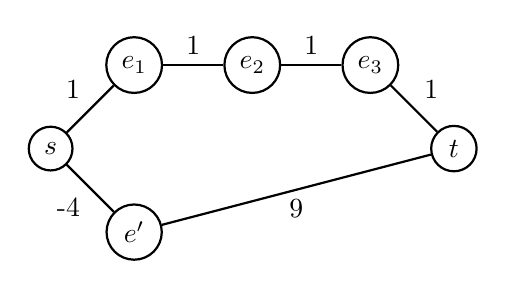
\begin{tikzpicture}[node distance={15mm}, thick, main/.style = {draw, circle}] 
      \node[main] (1) {$s$};

      \node[main] (2) [above right of=1] {$e_1$};

      \node[main] (4) [right of=2] {$e_2$};

      \node[main] (6) [right of=4] {$e_3$};

      \node[main] (8) [below right of=6] {$t$};

      \node[main] (3) [below right of=1] {$e'$};

      \draw (1) -- node[above left] {1} (2);
      \draw (2) -- node[above] {1} (4);
      \draw (4) -- node[above] {1} (6);
      \draw (6) -- node[above right] {1} (8);

      \draw (1) -- node[below left] {-4} (3);
      \draw (3) -- node[below] {9} (8);
    \end{tikzpicture}
  \end{center}

  In this case, we can clearly see that the shortest path is the top one with a
  total weight of $4$. Now let's see what happens when we add a weight of $4$ to
  every edge.

  \begin{center}
    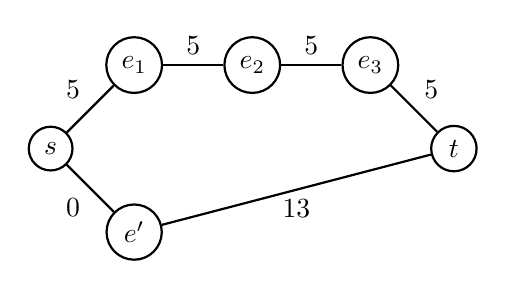
\begin{tikzpicture}[node distance={15mm}, thick, main/.style = {draw, circle}] 
      \node[main] (1) {$s$};

      \node[main] (2) [above right of=1] {$e_1$};

      \node[main] (4) [right of=2] {$e_2$};

      \node[main] (6) [right of=4] {$e_3$};

      \node[main] (8) [below right of=6] {$t$};

      \node[main] (3) [below right of=1] {$e'$};

      \draw (1) -- node[above left] {5} (2);
      \draw (2) -- node[above] {5} (4);
      \draw (4) -- node[above] {5} (6);
      \draw (6) -- node[above right] {5} (8);

      \draw (1) -- node[below left] {0} (3);
      \draw (3) -- node[below] {13} (8);
    \end{tikzpicture}
  \end{center}

  Now the top path has a total weight of $20$, and the bottom one has a weight
  of $13$, so this is {\bf not} the same graph as the one we started with.

  What this shows us is that we can't simply solve this problem by offsetting
  the weights of such a graph.

  \subsubsection{The Problem}

  Given a digraph $G = (V, E)$ with edge weight $c_{uv}$ for each edge $(u, v)
  \in E$. We're also given vertices $s, t \in V$. What is {\it a} minimum cost
  path from $s$ to $t$? The cost of the path is the sum of the costs of
  the edges on that path.

  Why should we care about negative edge weights? well it could be the case that
  in certain scenarios. For example, what if the edges represent financial
  transactions? In that case, we would want to make the total cost as low as
  possible.

  \subsubsection{Assumption}

  {\it We're going to make an assumption to make the problem well defined}.

  {\bf $G$ does not contain negative cost cycles}. The reason we want to avoid
  this is because, if $G$ did have negative cost cycles, you could just go
  around in circle in that cycle to make your weight arbitrarily low.

  \note {
    Our graph {\it may} have cycles! But no {\it negative cost} cycles.
  }

  \subsubsection{Approaches}

  To solve the problem, we could think of modifying Dijkstra's algorithm in some
  way. Unfortunately we can see that this does not work. Having negative edge
  weights means you can't simply consider ``one more edge". Let's look at an
  example.

  \example {
    In the following graph, the shortest path from $s$ to $v$ is not obvious. We
    would need to explore more of the graph to be able to find it.

    \begin{center}
      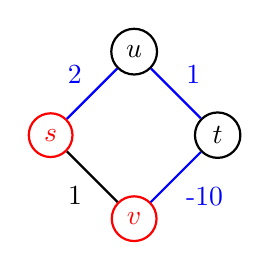
\begin{tikzpicture}[node distance={15mm}, thick, main/.style = {draw, circle}] 
        \node[main] (1) {$u$};
        \node[main] (2) [below left of=1, red] {$s$};
        \node[main] (3) [below right of=1] {$t$}; 
        \node[main] (4) [below left of=3, red] {$v$};

        \draw (1) [blue] -- node[above left] {2} (2) ;
        \draw (1) [blue]-- node[above right] {1} (3);

        \draw (3) [blue] -- node[below right] {-10} (4);
        \draw (2) -- node[below left] {1} (4);
        % \draw[red, very thick] (4) -- node[below] {2} (5);
        % \draw (2) -- node[above] {7} (5);
      \end{tikzpicture}
    \end{center}
  }

  \subsection{Bellman-Ford Algorithm}

  {\bf Main Idea}: Let $\opt(i, v)$ be the minimum cost of a path from $v$ to
  $t$ using at most $i$ edges.

  By limiting the number of edges at each step, we have our sub-problem!

  Why does this work? Why isn't the memo too big?
  \begin{itemize}
    \item There's only $n$ vertices $V$
    \item The minimum cost path is simple, so only need to consider {\it paths
      of length $\le n - 1$}
  \end{itemize}

  \QUESTION{} Why do we care about this?

  {\bf Question}: Does the min-cost path for $\opt(i, v)$ use all $i$ edges?

  \begin{itemize}
    \item {\bf No}: Then $\opt(i, v) = \opt(i - 1, v)$, since we don't use all
      $i$ edges, so the solution should be the same using one less edge.

    \item {\bf Yes}: Then $\opt(i, v) = \min_{u \in V}\big(\opt(i - 1, u) +
      c_{uv}\big)$.

      Here we consider the optimal way to get to a neighbor $u$ of $v$, and then
      look for the best way to get from $u$ to $v$.
  \end{itemize}


  {\bf Initial Conditions}

  \begin{itemize}
    \item $\opt(0, t) = 0$.

      $t$ is our {\it target} vertex, it's also right where we happen to be, so
      the cost to get to it is $0$.

    \item $\opt(0, v) = \infty$ for all $v \ne t$.

      If you want to get to any vertex other than $t$ in at most $0$ edges, you
      can't.

  \end{itemize}

  {\bf Goal}: Compute the shortest path from $s$ to $t$ using {\it at most} $n -
  1$ edges. In other words, $\opt(n - 1, s)$.

  \subsubsection{Pseudocode}

  \begin{lstlisting}
BellmanFord($G$, $c$, $s$, $t$):
  let $n$ be the number of vertices of $G$
  let $M$ be an $n \times n$ array

  for all $v \ne t$:
    $M[0, t] = 0$ 
    $M[0, v] = \infty$ 
  end

  for $i = 1$ to $n - 1$:
    for $v \in V$:
      $M[i, v] = \min \{ M[i - 1, v], \min_{u \in V}(M[i - 1, u] + c_{uv}) \}$
    end
  end

  return $M[n - 1, s]$
end
  \end{lstlisting}

  Where

  \begin{itemize}
    \item $G$ is our graph.
    \item $c$ is the list of edge weights of $G$.
    \item $s$ is our start vertex.
    \item $t$ is our target vertex.
  \end{itemize}


  \subsubsection{Running Time}

  We definitely have a $\O(n^3)$ upper bound. We can do better than this though,
  by noticing that the cost of line 12 is $\O(\outdeg(v) + 1)$.

  So the total running time is

  \[
    \O\Big(n \cdot \sum_{v \in V} (\outdeg(v) + 1)\Big) = \O(n(m + n))
  \]

  If the graph is sparse, this is quite good.

  \subsubsection{Negative Cycles}

  If we do have negative cycles, running this algorithm would continue to find
  lower and lower bounds for the path. At some point we can stop, but how do we
  know if there is one?

  Bellman-Ford will find a negative cycle if one exists, provided that

  \begin{enumerate}
    \item there is a path from the cycle to $t$, where we're trying to go
    \item it runs long enough to see the cycle.

      \note {
        This is not necessarily the case: what if the whole graph is one big
        cycle? Then you'll never figure this out because you'll get to your
        destination before noticing the cycle.
      }

  \end{enumerate}

  \Lemma {
    For any directed graph $G$, there exists a digraph $G'$ with {\it one more}
    vertex than $G$ such that $G'$ has a path from a negative cycle to $t$, if
    and only if $G$ has a negative cycle.
  }
  {
    {\it This proof isn't formal, but let's describe the main idea.}

    You have some graph $G$. Create a new vertex $t$, and add an edge from all
    the vertices in $G$, to this new vertex $t$.

    Now if there was a negative cycle in $G$, its {\it definitely} connected to
    $t$.
  }

  This solves the first of the two problems. Now we need to make sure that our
  algorithm can see the cycle, provided that there is one.

  Remember when we considered that the whole graph was one big cycle? Well we
  only needed to run Bellman-Ford one more time (on all $n$ edges instead of $n
  - 1$) to notice that we're in a cycle. It turns out that this is completely
  generic, and will always work.

  \Lemma {
    A digraph has no negative-weight cycles {\bf if and only if} $\opt(n - 1, v)
    = \opt(n, v)$ for all vertices $v$.

    {\it here, $n$ is the number of vertices in $G'$, not $G$.}

    In other words, we add {\it one more} row to the memo. If the last row is
    the same as the second to last row, then there are no negative cycles. If it
    {\it is} different, then there {\it is} a negative cycle.
  }
  {
    If there are no negative weight cycles, then this follows from the
    correctness of Bellman-Ford (the result of one more search should not
    change.)

    Conversely, if it is the case that $\opt(n - 1, v) = \opt(n, v)$ for all
    vertices $v$, then by induction, it {\it must} be the case that $\opt(n, v)
    = \opt(k, v)$ for all $k \ge n - 1$.

    However, if there were a negative cycle, then $\opt(k, v)$ could become
    arbitrarily small (because you could just go around the cycle as many times
    as you'd like.)

    {\it But you don't need to go around the cycle a million times to see if
    there is a cycle! You just need one more iteration of Bellman-Ford, and you
    check if things have changed.}
  }


  {\bf Why did we add the vertex $t$?}

  Well remember that we always want to get to $t$. So we created a graph that
  you can reach from all vertices. By making sure we create such a graph, we
  make sure that Bellman-Ford will always explore the whole graph to check what
  the best way to get to $t$ is.



  \newpage
  \section{Network Flow}

  \btw {
    We're still talking about graph algorithms, but ultimately, this is a new
    style of algorithm.

    We're going to try to find augmenting paths in graphs. This is a really
    powerful algorithmic idea, and sometimes it's not obvious where it might
    show up.
  }

  \Definition{Flow Network}
  {
    We're going to have this notion of a {\bf flow network}. This is a digraph
    $G = (V, E)$ with

    \begin{itemize}
      \item A designated {\bf source} vertex $s \in V$. This is a vertex with no
        edges pointing into it.

        \[
          \indeg(s) = 0
        \]

      \item A designated {\bf sink} vertex $t \in V$. This is a vertex with
        nothing coming out of it.

        \[
          \outdeg(t) = 0
        \]

      \item A {\bf capacity} $C_e \ge 0$ for all edges $e \in E$.

        These are essentially the weights of the edges. We also assume that they
        are {\bf integers}.

    \end{itemize}
  }

  For the problem that we're considering, there is only one sink and one
  source. Generally, there's no reason why we couldn't have multiple vertices
  with in-degree $0$, or out-degree $0$.

  Let's look at an example flow network.

  \example {
    \begin{center}
      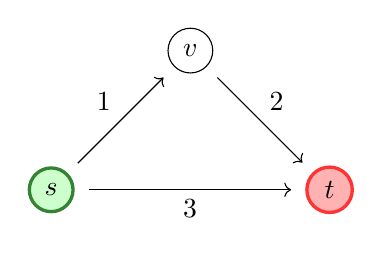
\begin{tikzpicture} 
        \node[main] (v) {$v$};
        \node[main, source] (s) [below left of=v] {$s$};
        \node[main, sink] (t) [below right of=v] {$t$};

        \draw [->] (s) -- node[above left] {1} (v);
        \draw [->] (v) -- node[above right] {2} (t);
        \draw [->] (s) -- node[below] {3} (t);
      \end{tikzpicture}
    \end{center}
  }

  \Definition {Flow} {
    A {\bf flow} is a function $f: E \to \R^+$ satisfying

    \begin{itemize}
      \item {\bf Capacity} conditions $0 \le f(c) \le C_e$ for all $e \in E$

        {\it An edge can't pump more liquid than its $C_e$ value}.

      \item {\bf Conservation} conditions.

        \[
          f^\text{in} (v) = f^\text{out} (v)
        \]

        For all vertices $v$, {\bf except the source $s$ and sink $t$}.

        {\it An edge transfers as much flow as is sent into it}.
    \end{itemize}

    Here, $f^\text{in} (v)$ is the sum of all the flows going into $v$, and
    $f^\text{out}(v)$ is the sum of the flows going out of $v$.

    \[
      f^\text{in} (v) = \sum_{e \text{ into } v} f(e)
    \]

    \[
      f^\text{out} (v) = \sum_{e \text{ out of } v} f(e)
    \]
  }

  \subsection{Flow Examples}

  Let's look at an example of a flow.

  \example {
    This is a flow that satisfies the conditions above.

    \begin{center}
      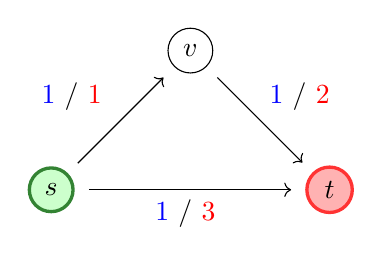
\begin{tikzpicture}

        \node[main] (v) {$v$};
        \node[main, source] (s) [below left of=v] {$s$};
        \node[main, sink] (t) [below right of=v] {$t$};

        \draw [->] (s) -- node[above left] {\fc{1}{1}} (v);
        \draw [->] (v) -- node[above right] {\fc{1}{2}} (t);
        \draw [->] (s) -- node[below] {\fc{1}{3}} (t);
      \end{tikzpicture}
    \end{center}
  }

  The edge weights are represented as

  \begin{center}
    \fc{flow value}{capacity}
  \end{center}

  Note that this was not the best flow!

  \example {
    This is.

    \begin{center}
      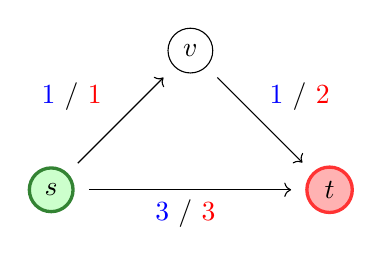
\begin{tikzpicture}
        \node[main] (2) {$v$};
        \node[main, source] (1) [below left of=2] {$s$};
        \node[main, sink] (3) [below right of=2] {$t$};

        \draw [->] (1) -- node[above left] {\fc{1}{1}} (2);
        \draw [->] (2) -- node[above right] {\fc{1}{2}} (3);
        \draw [->] (1) -- node[below] {\fc{3}{3}} (3);
      \end{tikzpicture}
    \end{center}

    Notice that the edge from $v$ to $t$ is still at flow value $1$, even if it
    can handle $2$. That's because only $1$ is coming into it.
  }

  We'll spend a lot of time trying to find the best possible flow of these
  graphs.

  \subsection{Invalid Flow Examples}

  Notice that there are also {\it invalid flows}.

  \example {
    \begin{center}
      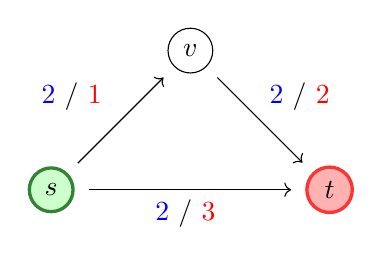
\begin{tikzpicture}
        \node[main] (2) {$v$};
        \node[main, source] (1) [below left of=2] {$s$};
        \node[main, sink] (3) [below right of=2] {$t$};

        \draw [->] (1) -- node[above left] {\fc{2}{1}} (2);
        \draw [->] (2) -- node[above right] {\fc{2}{2}} (3);
        \draw [->] (1) -- node[below] {\fc{2}{3}} (3);
      \end{tikzpicture}
    \end{center}

    The graph above is wrong because it doesn't respect the {\bf capacity} constraint.

    \begin{center}
      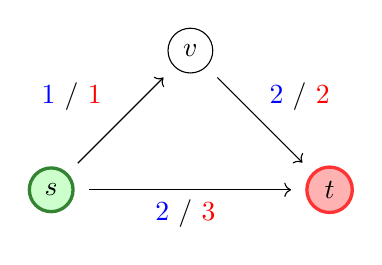
\begin{tikzpicture}
        \node[main] (2) {$v$};
        \node[main, source] (1) [below left of=2] {$s$};
        \node[main, sink] (3) [below right of=2] {$t$};

        \draw [->] (1) -- node[above left] {\fc{1}{1}} (2);
        \draw [->] (2) -- node[above right] {\fc{2}{2}} (3);
        \draw [->] (1) -- node[below] {\fc{2}{3}} (3);
      \end{tikzpicture}
    \end{center}

    The graph above is wrong because it doesn't respect the {\bf conservation}
    constraint.
  }

  \Definition{} {
    The {\bf value} of a flow $v(f) = f^\text{out}(s)$ is the total flow that's
    leaving $s$.
  }

  \subsection{Finding a maximum flow}

  What happens if we try to be greedy? Spoiler alert: it won't work. Let's see
  why.

  Here's the strategy:

  \begin{enumerate}
    \item Find an $s \to t$ path (using your favorite path finding algorithm)
    \item Send as much flow along it as possible.
  \end{enumerate}
  
  Consider the following flow generated by the greedy rule.

  \begin{center}
    \begin{tikzpicture}
      \node[main] (u) {$u$};
      \node[main, source] (s) [below left of=u] {$s$};
      \node[main, sink] (t) [below right of=u] {$t$};
      \node[main] (v) [below left of=3] {$v$};

      \draw [->, selected] (s) -- node[above left] {2} (u);
      \draw [->] (u) -- node[above right] {1} (t);
      \draw [->] (s) -- node[below left] {1} (v);
      \draw [->, selected] (v) -- node[below right] {2} (t);
      \draw [->, selected] (u) -- node[right] {3} (v);
    \end{tikzpicture}
  \end{center}

  We can be more precise, here are the flow / capacities.

  \begin{center}
    \begin{tikzpicture}
      \node[main] (u) {$u$};
      \node[main, source] (s) [below left of=u] {$s$};
      \node[main, sink] (t) [below right of=u] {$t$};
      \node[main] (v) [below left of=3] {$v$};

      \draw [->, selected] (s) -- node[above left] {\fc{2}{2}} (u);
      \draw [->] (u) -- node[above right] {\fc{0}{1}} (t);
      \draw [->] (s) -- node[below left] {\fc{0}{1}} (v);
      \draw [->, selected] (v) -- node[below right] {\fc{2}{2}} (t);
      \draw [->, selected] (u) -- node[right] {\fc{2}{3}} (v);
    \end{tikzpicture}
  \end{center}

  We get that the flow value at our sink $t$ is 2. But notice that we're not
  using edges $s \to v$ or $u \to t$. Here's a better flow instead.

  \begin{center}
    \begin{tikzpicture}
      \node[main] (u) {$u$};
      \node[main, source] (s) [below left of=u] {$s$};
      \node[main, sink] (t) [below right of=u] {$t$};
      \node[main] (v) [below left of=3] {$v$};

      \draw [->, selected] (s) -- node[above left] {\fc{2}{2}} (u);
      \draw [->, selected] (u) -- node[above right] {\fc{1}{1}} (t);
      \draw [->, selected] (s) -- node[below left] {\fc{1}{1}} (v);
      \draw [->, selected] (v) -- node[below right] {\fc{2}{2}} (t);
      \draw [->, selected] (u) -- node[right] {\fc{1}{3}} (v);
    \end{tikzpicture}
  \end{center}

  Doing this, we still respect the capacity and conservation conditions, and
  we get a flow value of 3 at our sink. This should convince you that the greedy
  approach is sub-optimal.


  This is great and all but how did we come up with this better example?
  We want a general way to send as much flow as possible from $s$ to $t$ that
  will work in general. The general strategy that we'll use to do this stems
  from a simple idea. We'll allow ourselves to not only send flow forward along
  an edge, but also backwards. Sending flow backwards along an edge is analogous
  to decreasing the flow in the forward direction.

  It should make sense that we should only allow ourselves to do this for edges
  that have flow in the forwards direction to begin with.

  \subsection{Residual Networks}

  To get around this issue, we're going to consider forward edges and backward
  edges in {\bf residual networks}.

  \Definition {Residual Network} {
    Given a flow network and a flow $f$, their {\bf residual flow network} works as
    follows

    \begin{itemize}
      \item The vertices are those of the original flow network.

      \item {\bf Forward Edges}: For each edge $e$ with $f(e) < C_e$, include
        the edge $e$ with capacity $C_e - f(e)$.

        In this case, we're not using $e$ to its full capacity. 

      \item {\bf Backward Edges}: For each edge $e = (u, v)$ with positive flow
        value $f(e) > 0$, include the edge $(v, u)$ with capacity $f(e)$.

        We should allow ourselves to decrease the flow along $e$ by at most
        $f(e)$.
    \end{itemize}
  }

  \note {
    A Residual Flow Network is {\bf only} defined for a {\it particular flow!}
  }

  We want to send as much flow from the start to the destination. 

  The residual flow network ``flows backwards through the graph".

  Let's look at an example

  \example {
    Consider the following flow network.

    \begin{center}
      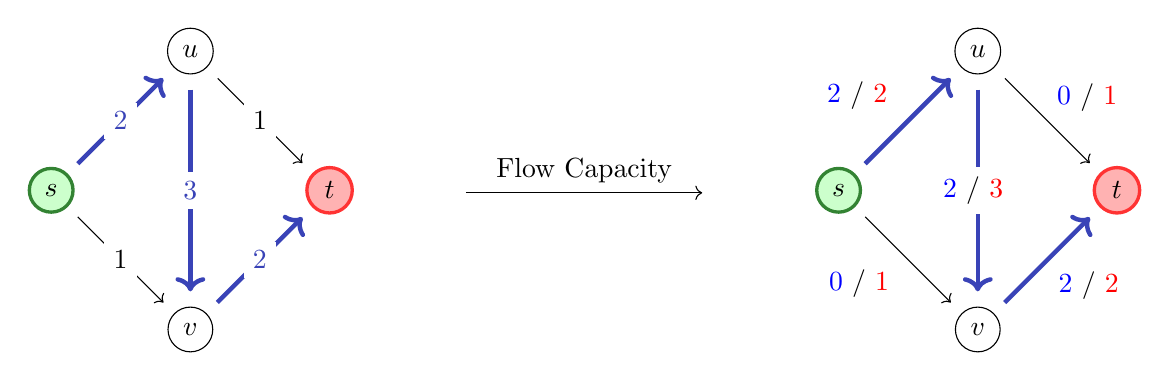
\begin{tikzpicture}
        \begin{scope}[xshift=-5cm]
          \node[main] (u) {$u$};
          \node[main, source] (s) [below left of=u] {$s$};
          \node[main, sink] (t) [below right of=u] {$t$};
          \node[main] (v) [below left of=t] {$v$};

          \draw [->, selected] (s) -- node[mid] {2} (u);
          \draw [->] (u) -- node[mid] {1} (t);
          \draw [->] (s) -- node[mid] {1} (v);
          \draw [->, selected] (v) -- node[mid] {2} (t);
          \draw [->, selected] (u) -- node[mid] {3} (v);
        \end{scope}

        \begin{scope}[xshift=5cm]
          \node[main] (_u) {$u$};
          \node[main, source] (_s) [below left of=_u] {$s$};
          \node[main, sink] (_t) [below right of=_u] {$t$};
          \node[main] (_v) [below left of=_t] {$v$};

          \draw [->, selected] (_s) -- node[above left] {\fc{2}{2}} (_u);
          \draw [->] (_u) -- node[above right] {\fc{0}{1}} (_t);
          \draw [->] (_s) -- node[below left] {\fc{0}{1}} (_v);
          \draw [->, selected] (_v) -- node[below right] {\fc{2}{2}} (_t);
          \draw [->, selected] (_u) -- node[mid] {\fc{2}{3}} (_v);
        \end{scope}

        \draw [->, above, yshift=-1.8cm] (-1.5,0) -- node[above] {Flow Capacity} (1.5,0);
      \end{tikzpicture}
    \end{center}

    Let's construct the residual network of this particular flow using the
    rules from the last lecture.

    \begin{center}
      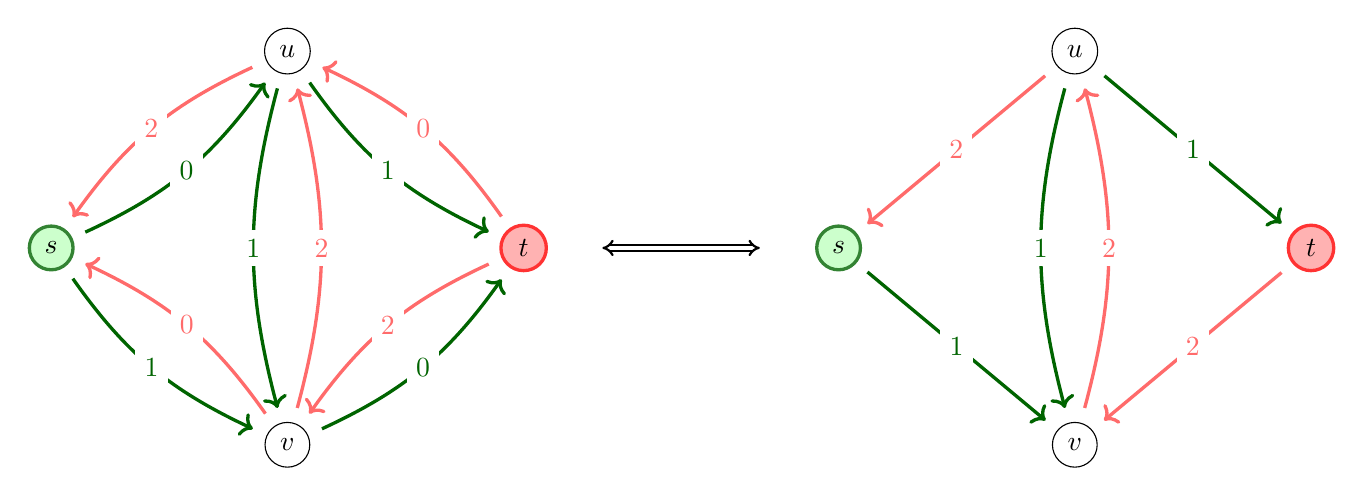
\begin{tikzpicture}[
        node distance={3.5cm},
      ]
        \begin{scope}[xshift=-5cm]
          \node[main] (u) at (0, 0) {$u$};
          \node[main] (v) at (0, -5) {$v$};
          \node[main, source] at (-3, -2.5) (s) {$s$};
          \node[main, sink] (t) at (3, -2.5) {$t$};

          \draw [<-, backwards] (s) to[bend left=15] node[mid] {2} (u);
          \draw [->, forwards] (s) to[bend right=15] node[mid] {0} (u);

          \draw [<-, backwards] (s) to[bend left=15] node[mid] {0} (v);
          \draw [->, forwards] (s) to[bend right=15] node[mid] {1} (v);

          \draw [<-, backwards] (u) to[bend left=15] node[mid] {2} (v);
          \draw [->, forwards] (u) to[bend right=15] node[mid] {1} (v);

          \draw [<-, backwards] (u) to[bend left=15] node[mid] {0} (t);
          \draw [->, forwards] (u) to[bend right=15] node[mid] {1} (t);

          \draw [<-, backwards] (v) to[bend left=15] node[mid] {2} (t);
          \draw [->, forwards] (v) to[bend right=15] node[mid] {0} (t);
        \end{scope}

        \begin{scope}[xshift=5cm]
          \node[main] (u) at (0, 0) {$u$};
          \node[main] (v) at (0, -5) {$v$};
          \node[main, source] at (-3, -2.5) (s) {$s$};
          \node[main, sink] (t) at (3, -2.5) {$t$};

          \draw [<-, backwards] (s) to node[mid] {2} (u);

          \draw [->, forwards] (s) to node[mid] {1} (v);

          \draw [<-, backwards] (u) to[bend left=15] node[mid] {2} (v);
          \draw [->, forwards] (u) to[bend right=15] node[mid] {1} (v);

          \draw [->, forwards] (u) to node[mid] {1} (t);

          \draw [<-, backwards] (v) to node[mid] {2} (t);
        \end{scope}

        \draw[implies-implies, double equal sign distance, thick] (-1, -2.5)
          -- (1, -2.5);
      \end{tikzpicture}
    \end{center}

    Now, we can use the residual network to send the following flow

    \begin{center}
      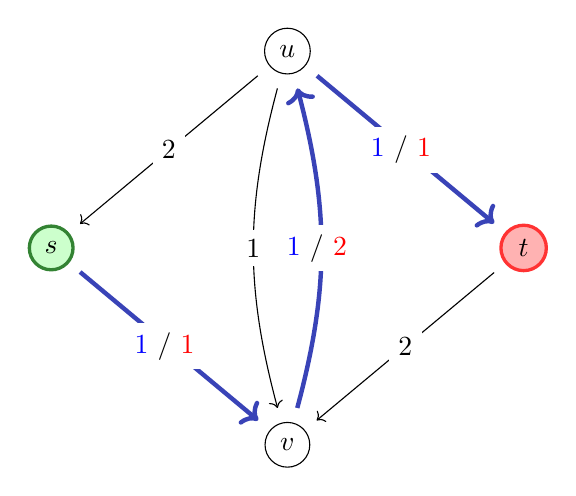
\begin{tikzpicture}
        \node[main] (u) at (0, 0) {$u$};
        \node[main] (v) at (0, -5) {$v$};
        \node[main, source] at (-3, -2.5) (s) {$s$};
        \node[main, sink] (t) at (3, -2.5) {$t$};

        \draw [<-] (s) to node[mid] {2} (u);

        \draw [->, selected] (s) to node[mid] {\fc{1}{1}} (v);

        \draw [<-, selected] (u) to[bend left=15] node[mid] {\fc{1}{2}} (v);
        \draw [->] (u) to[bend right=15] node[mid] {1} (v);

        \draw [->, selected] (u) to node[mid] {\fc{1}{1}} (t);

        \draw [<-] (v) to node[mid] {2} (t);
      \end{tikzpicture}
    \end{center}

    What we've done here is that we've {\bf augmented} the flow! We used the
    residual network of our original flow and found a flow that we could send
    through it that we can now use to update our original flow.

    \begin{center}
      \begin{tikzpicture}
        \node[main] (u) {$u$};
        \node[main, source] (s) [below left of=u] {$s$};
        \node[main, sink] (t) [below right of=u] {$t$};
        \node[main] (v) [below left of=3] {$v$};

        \draw [->, selected] (s) -- node[above left] {\fc{2}{2}} (u);
        \draw [->, selected] (u) -- node[above right] {\fc{1}{1}} (t);
        \draw [->, selected] (s) -- node[below left] {\fc{1}{1}} (v);
        \draw [->, selected] (v) -- node[below right] {\fc{2}{2}} (t);
        \draw [->, selected] (u) -- node[mid] {\fc{1}{3}} (v);
      \end{tikzpicture}
    \end{center}

    This is the optimal flow that we found earlier!
  }

  This is exactly what our algorithm is going to do. We're going to start from
  zero flow, construct the residual network, send as much flow as possible along
  some path, augment the flow, construct the new residual network, etc... Until
  we can't send anymore flow from $s$ to $t$.

  \note {
    It turns out that this approach is optimal. By repeating this process, we
    {\it will} find the optimal flow from $s$ to $t$.
  }

  \Definition {Augmenting Path} {
    An {\bf Augmenting Path} is a simple path from $s$ to $t$ in the residual
    network, with positive capacity.
  }

  \subsection{The Ford-Fulkerson Algorithm}

  Here are the steps we need.

  \begin{enumerate}
    \item {\bf Find an Augmenting Path.}

      We can do this using BFS or some other path-finding algorithm. It doesn't
      actually matter if we don't find the {\it best} path from $s$ to $t$
      here, any path will work.

    \item {\bf Augment the Flow.}

      For a path $P$ and a flow $f$, we let $\text{bottleneck}(P, f)$ be the
      smallest capacity of any edge on $P$, {\bf in the residual network
      corresponding to $f$}.

      Let's look at exactly how this works.

      \begin{lstlisting}
Augment($f$, $P$):
  # done by walking along the path and
  # finding the minimum capacity
  let $b$ = bottleneck($P$, $f$)

  for $e = (u, v)$ along $P$:
    if $e$ is a forward edge:
      increase $f(e)$ by $b$
    else:
      # $e$ is a backwards edge

      let $e' = (v, u)$
      decrease $f(e')$ by $b$
  end
end
      \end{lstlisting}

      To figure out if an edge is forwards or backwards, you compare it to the
      edge from the original flow network. Remember, the graph we pass to
      \texttt{Augment} is the graph of the residual network, so its edges might
      differ from the original graph.

      \Lemma {
        \texttt{Augment($f$, $P$)} produces a valid flow.
      }
      {
        To prove this, we have to prove that \texttt{Augment($f$, $P$)} respects
        the capacity, and conservation constraints on the original graph.

        {\bf Capacity}

        Suppose $e$ is a forward edge, we increase the flow by $b$, and every edge
        on $P$ has residual capacity at least $b$ (in other words, every edge along
        $P$ can still take at least $b$ more flow) so we still satisfy the capacity
        constraint.

        If $e$ is a backward edge, we decrease the capacity by $b$. Since $b$ is at
        most $f(e)$, we never decrease the flow by more than the maximum possible,
        so the resulting flow is non-negative. Again, we satisfy the capacity
        constraint.

        {\bf Conservation}

        Whenever we add flow into an internal vertex (not the source or the
        sink), then we add the same flow going out.
      }
    
  \end{enumerate}

  Now we're ready to see the complete algorithm.

  \subsubsection{Algorithm}

  \begin{lstlisting}
MaxFlow($G$, $C$, $s$, $t$)
  let $f(e) = 0$ for all edges $e$ of $G$

  while there is a simple path $P$ from $s$ to $t$
  in the residual network of flow $f$:
    update $f$ to Augment($f$, $P$)
    update the residual network to use the new flow
  end

  return $f$
end
  \end{lstlisting}

  Where
  \begin{itemize}
    \item $G$ is our graph
    \item $C$ stores the capacity of each edge
    \item $s$ is our source vertex
    \item $t$ is our sink vertex
  \end{itemize}

  \subsubsection{Proof of Termination}

  How do we know that this algorithm terminates? How do we know that it finds
  the max flow?

  This is actually quite subtle, this algorithm actually could run indefinitely,
  {\it if we had not restricted ourselves to integer capacities}.

  \Lemma {
    The value of the flow strictly increases, at every step of the algorithm.
  }
  {
    The first edge of augmenting path $P$ starts from $s$. The flow along this
    edge is increased by the bottleneck capacity $b > 0$. Since $P$ is simple,
    this is the only edge of $P$ that includes $s$. So the value of the flow is
    increased by $b$.
  }

  \Lemma {
    At each step of the algorithm, the flow values and the residual capacities
    are all integers.
  }
  {
    This just simply follows from the basic fact that $\Z$ is closed addition.

    In other words, if you subtract an integer from an integer, you get an
    integer. If you add an integer to an integer, you get another integer.
  }

  From these two lemmas, we get that the flow increases by at least 1 at each
  step. Since the larger possible flow value is at most

  \[
    C = \sum_{e} C_e
  \]

  Where $e$ is an edge leaving $s$.

  This is finite, so we eventually must reach it. Thus the algorithm terminates.

  \note {
    Although $C$ is the maximum flow, it might not be achievable.
  }

  \subsubsection{Running Time}

  Additionally, $C$ is an upper bounds for the number of iterations that the
  algorithm performs.

  Since each pass through the loop can be implemented in time $\O(m + n)$, the
  overall running time is $\O(C(n + m))$.

  \subsection{Maximum Flows \& Minimal Cuts}

  We saw that $C$ was an upper bound for the maximum flow, but we can find other
  bounds for the flow by considering various types of {\it cuts}. Recall the
  definition of a cut: a bipartition of the vertices.

  \Definition {} {
    We call an cut an $s$-$t$ cut if $s \in A$ and $t \in B$.
  }

  In a flow network. The capacity of an $s$-$t$ cut is the total capacity of all
  edges leaving $A$.

  \[
    C(A, B) = \sum_{e \text{ out of } A} C_e
  \]

  We only look at the edges that go from the $A$ part of the cut, to the $B$
  part of the cut.

  \example {
    Let's look at our example from earlier.

    \begin{center}
      \begin{tikzpicture}
        \node[main] (u) {$u$};
        \node[main, source] (s) [below left of=u] {$s$};
        \node[main, sink] (t) [below right of=u] {$t$};
        \node[main] (v) [below left of=3] {$v$};

        \draw [->] (s) -- node[mid] {2} (u);
        \draw [->] (u) -- node[mid] {1} (t);
        \draw [->] (s) -- node[mid] {1} (v);
        \draw [->] (v) -- node[mid] {2} (t);
        \draw [->] (u) -- node[mid] {3} (v);
      \end{tikzpicture}
    \end{center}

    We can generate a cut by choosing any subset $A \subset V$ which includes
    $s$ and doesn't include $t$.

    \begin{center}
      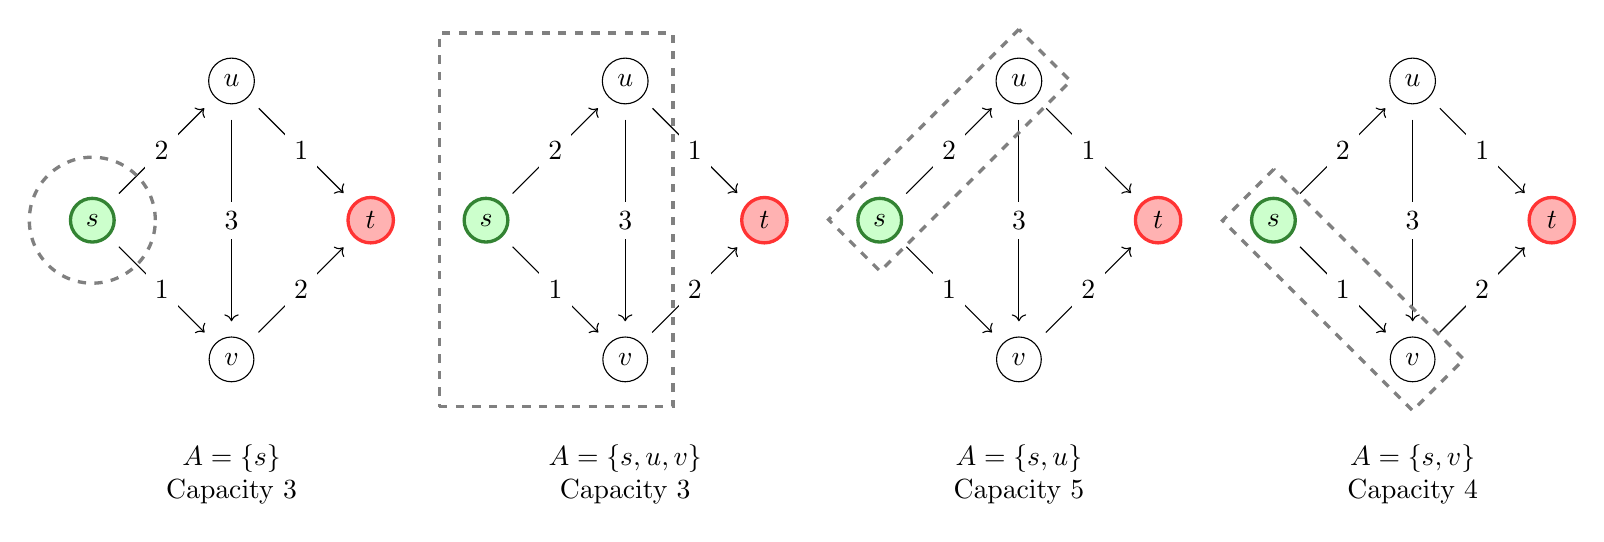
\begin{tikzpicture}[node distance={2.5cm}, baseline={(current bounding box.center)}]
        \begin{scope}[xshift=-7.5cm]
          \node[main] (u) {$u$};
          \node[main, source] (s) [below left of=u] {$s$};
          \node[main, sink] (t) [below right of=u] {$t$};
          \node[main] (v) [below left of=t] {$v$};

          \draw [->] (s) -- node[mid] {2} (u);
          \draw [->] (u) -- node[mid] {1} (t);
          \draw [->] (s) -- node[mid] {1} (v);
          \draw [->] (v) -- node[mid] {2} (t);
          \draw [->] (u) -- node[mid] {3} (v);

          \draw[draw=gray, dashed, very thick] (s) circle (0.8);

          \node at (0, -5) [align=center] {$A = \{s\}$ \\ Capacity $3$};
        \end{scope}

        \begin{scope}[xshift=-2.5cm]
          \node[main] (u) {$u$};
          \node[main, source] (s) [below left of=u] {$s$};
          \node[main, sink] (t) [below right of=u] {$t$};
          \node[main] (v) [below left of=t] {$v$};

          \draw [->] (s) -- node[mid] {2} (u);
          \draw [->] (u) -- node[mid] {1} (t);
          \draw [->] (s) -- node[mid] {1} (v);
          \draw [->] (v) -- node[mid] {2} (t);
          \draw [->] (u) -- node[mid] {3} (v);

          \node [draw=gray, dashed, very thick, fit=(s)(u)(v)] {};

          \node at (0, -5) [align=center] {$A = \{s, u, v\}$ \\ Capacity $3$};
        \end{scope}

        \begin{scope}[xshift=2.5cm]
          \node[main] (u) {$u$};
          \node[main, source] (s) [below left of=u] {$s$};
          \node[main, sink] (t) [below right of=u] {$t$};
          \node[main] (v) [below left of=t] {$v$};

          \draw [->] (s) -- node[mid] {2} (u);
          \draw [->] (u) -- node[mid] {1} (t);
          \draw [->] (s) -- node[mid] {1} (v);
          \draw [->] (v) -- node[mid] {2} (t);
          \draw [->] (u) -- node[mid] {3} (v);

          \node [draw=gray, dashed, very thick, rotate fit=45, fit=(s)(u)] {};

          \node at (0, -5) [align=center] {$A = \{s, u\}$ \\ Capacity $5$};
        \end{scope}

        \begin{scope}[xshift=7.5cm]
          \node[main] (u) {$u$};
          \node[main, source] (s) [below left of=u] {$s$};
          \node[main, sink] (t) [below right of=u] {$t$};
          \node[main] (v) [below left of=t] {$v$};

          \draw [->] (s) -- node[mid] {2} (u);
          \draw [->] (u) -- node[mid] {1} (t);
          \draw [->] (s) -- node[mid] {1} (v);
          \draw [->] (v) -- node[mid] {2} (t);
          \draw [->] (u) -- node[mid] {3} (v);

          \node [draw=gray, dashed, very thick, rotate fit=45, fit=(s)(v)] {};

          \node at (0, -5) [align=center] {$A = \{s, v\}$ \\ Capacity $4$};
        \end{scope}
      \end{tikzpicture}
    \end{center}
  }

  What we'll show next time is that the capacities of these cuts will give us
  upper bounds on the flow value.

  For any $S \subseteq V$, let $f^\text{in}(S) = \sum_{e \text{ into } S} f(e)$,
  and $f^\text{out}(S) = \sum_{e \text{ out of } S} f(e)$.

  Consider the following examples

  \begin{center}
    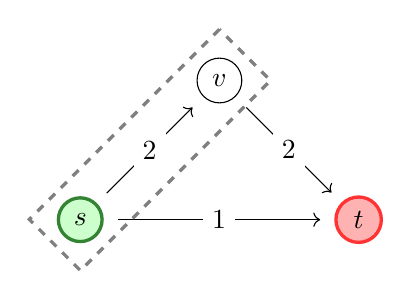
\begin{tikzpicture}
      \node[main] (v) {$v$};
      \node[main, source] (s) [below left of=v] {$s$};
      \node[main, sink] (t) [below right of=v] {$t$};

      \draw [->] (s) -- node[mid] {2} (v);
      \draw [->] (v) -- node[mid] {2} (t);
      \draw [->] (s) -- node[mid] {1} (t);

      \node [draw=gray, dashed, very thick, rotate fit=45, fit=(s)(v)] {};
    \end{tikzpicture}

    This cut has $v(f) = f^\text{out}(A) - f^\text{in}(A) = 3$
  \end{center}

  \vspace{0.5in}

  \begin{center}
    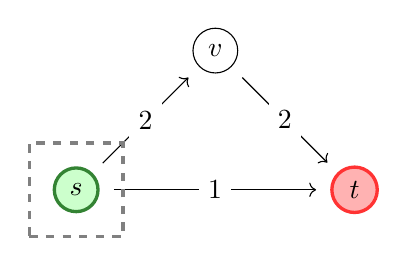
\begin{tikzpicture}
      \node[main] (v) {$v$};
      \node[main, source] (s) [below left of=v] {$s$};
      \node[main, sink] (t) [below right of=v] {$t$};

      \draw [->] (s) -- node[mid] {2} (v);
      \draw [->] (v) -- node[mid] {2} (t);
      \draw [->] (s) -- node[mid] {1} (t);

      \node [draw=gray, dashed, very thick, fit=(s)] {};
    \end{tikzpicture}

    This cut also has $v(f) = f^\text{out}(A) - f^\text{in}(A) = 3$
  \end{center}

  We'll show that this always holds.

  \Lemma {
    Let $f$ be any $s$-$t$ cut flow, and let $(A, B)$ be any $s$-$t$ cut. Then
    $v(f) = f^\text{out}(A) - f^\text{in}(A)$.
  }
  {
    By definition, $v(f) =  f^\text{out}(S) - f^\text{in}(S) = f^\text{out}(S)$
    since $f^\text{in}(S) = 0$. For any internal vertex $v$. But recall that for
    any vertex $v$

    \[
      f^\text{out}(v) - f^\text{in}(v) = 0
    \]

    But $v(f) = \sum_{v \in A} (f^\text{out}(v) - f^\text{in}(v))$. Now there
    are three cases

    \begin{itemize}
      \item If $e$ has both ends in $A$, it has a net zero contribution.
      \item If $e$ goes out of $A$, only the plus term has any contribution.
      \item If $e$ goes into $A$, only the minus term has any contribution.
    \end{itemize}

    This implies that $v(f) = f^\text{out}(A) - f^\text{in}(A)$.
  }

  \Lemma {
    Let $f$ be any $s$-$t$ flow, and let $(A, B)$ be any $s$-$t$ cut.

    {\bf Claim}. $v(f) \le c(A, B)$
  }
  {
    We know from the previous lemma that

    \begin{align*}
      v(f) =&f^\text{out}(A) - f^\text{in}(A) \\
         \le&f^\text{out}(A) \\
           =& \sum_{e \text{ out of } A} f(e) \\
           \le&\sum_{e \text{ out of } A} C_e \\
           =&c(A, B)
    \end{align*}
  }

  Now if we vary over all possible cuts, we get a many of upper bounds. What
  we'll show is that, as we vary over all possible cuts and consider all these
  upper bounds, the minimum such upper bound will be {\it equal} to the maximum
  flow that we can push!

  

  \NamedTheorem {\subsection{Max-Flow Min Cut Theorem}}
  {
    For any flow network, the largest value of any flow {\it is} the minimum
    capacity of any cut.
  }
  {
    Let $f$ be a flow such that there is no $s$-$t$ path in its residual flow
    network.

    \btw {
      We know that such a flow exists because the Ford-Fulkerson algorithm will
      produce such a flow, in fact there might be multiple such flows.
    }

    Let $A$ be the set of vertices $v$ with an $s$-$v$ path in the residual
    network of $A$. Let $B = V \setminus A$.

    {\bf Claim}
    \[
      v(f) = c(A, B)
    \]

    Then, the theorem will follow since, by the lemma, the maximum flow $f$ is
    less than or equal to the minimum $c(A', B')$ for all cuts $(A', B')$.

    \begin{itemize}
      \item Why is $(A, B)$ an $s$-$t$ cut?

        Clearly, $s \in A$, additionally, there does not exist an $s$-$t$ path
        in the residual network, so $t$ must be in $B$.

      \item How do the flows relate to the capacities?

        Let's first consider an edge $e = (u, v)$ where $u \in A$, and $v \in
        B$.

        It must be the case that the flow along that edge is equal to its
        capacity. If it were not, then $e$ would have a forward edge in the
        residual network. If this were the case, you could make a path from $s$
        to $v$ and so $v$ should be in $A$.

        \QUESTION{} Why could you make a path from $v$ to $s$ though?

        Secondly, let's consider an edge $e' = (u', v')$ where $u' \in B$, and
        $v' \in A$.

        If $f(e') > 0$, then $(v', u')$ is a backward edge in the residual
        network. So the path from $s$ to $v'$ could be extended to an $s$-$u'$
        path, which is a contradiction. Thus $f(e') = 0$.
    \end{itemize}

    Therefore

    \begin{align*}
      v(f) =&f^\text{out}(A) - f^\text{in}(A) \\
      =&\sum_{e \text{ out of } A} C_e - \sum_{e \text{ into } A} 0 \\
      =&c(A, B)
    \end{align*}
  }

  \subsection{Bipartite Matching}

  Recall that a bipartite graph has a bipartition of the vertices such that all
  edges have one end in $A$ and the other in $B$.

  What we mean by a matching here is 
  \Definition {}
  {
    A {\bf matching} in $G$ is an edge subset $M \subseteq E$ such that each
    vertex appears in at most one edge of $M$.
  }

  We want to find a maximum matching, we're going to use max flow ideas.

  Let's consider the following bipartite graph.

  \begin{center}
    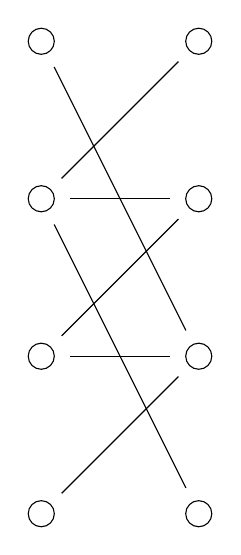
\begin{tikzpicture}
      \node[main] (1) at (0, 0) {};
      \node[main] (2) at (0, -2) {};
      \node[main] (3) at (0, -4) {};
      \node[main] (4) at (0, -6) {};

      \node[main] (5) at (2, 0)  {};
      \node[main] (6) at (2, -2) {};
      \node[main] (7) at (2, -4) {};
      \node[main] (8) at (2, -6) {};

      \draw [-] (1) -- (7);
      \draw [-] (2) -- (6);
      \draw [-] (3) -- (7);
      \draw [-] (4) -- (7);
      \draw [-] (2) -- (5);
      \draw [-] (3) -- (6);
      \draw [-] (2) -- (8);

      % \node[main, source] (s) at (-2, -3) {$s$};
      % \node[main, sink] (t) at (4, -3) {$t$};
      %
      % \draw [->] (s) -- (1);
      % \draw [->] (s) -- (2);
      % \draw [->] (s) -- (3);
      % \draw [->] (s) -- (4);
      % 
      % \draw [<-] (t) -- (5);
      % \draw [<-] (t) -- (6);
      % \draw [<-] (t) -- (7);
      % \draw [<-] (t) -- (8);
    \end{tikzpicture}
  \end{center}

  The maximum matching for this graph is the following.

  \begin{center}
    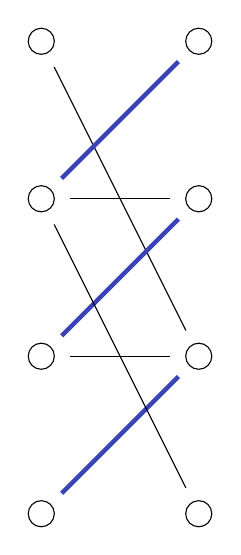
\begin{tikzpicture}
      \node[main] (1) at (0, 0) {};
      \node[main] (2) at (0, -2) {};
      \node[main] (3) at (0, -4) {};
      \node[main] (4) at (0, -6) {};

      \node[main] (5) at (2, 0)  {};
      \node[main] (6) at (2, -2) {};
      \node[main] (7) at (2, -4) {};
      \node[main] (8) at (2, -6) {};

      \draw [-] (1) -- (7);
      \draw [-] (2) -- (6);
      \draw [-] (3) -- (7);
      \draw [-, selected] (4) -- (7);
      \draw [-, selected] (2) -- (5);
      \draw [-, selected] (3) -- (6);
      \draw [-] (2) -- (8);

      % \node[main, source] (s) at (-2, -3) {$s$};
      % \node[main, sink] (t) at (4, -3) {$t$};
      %
      % \draw [->] (s) -- (1);
      % \draw [->] (s) -- (2);
      % \draw [->] (s) -- (3);
      % \draw [->] (s) -- (4);
      % 
      % \draw [<-] (t) -- (5);
      % \draw [<-] (t) -- (6);
      % \draw [<-] (t) -- (7);
      % \draw [<-] (t) -- (8);
    \end{tikzpicture}
  \end{center}

  We can't add anymore vertices here because if we did, we would be using some
  vertex twice, which we disallow.

  {\bf Question}: How can we find maximum matchings?

  {\bf Answer}: Network Flow.

  Consider the following network, where the capacity of all edges is one.

  \begin{center}
    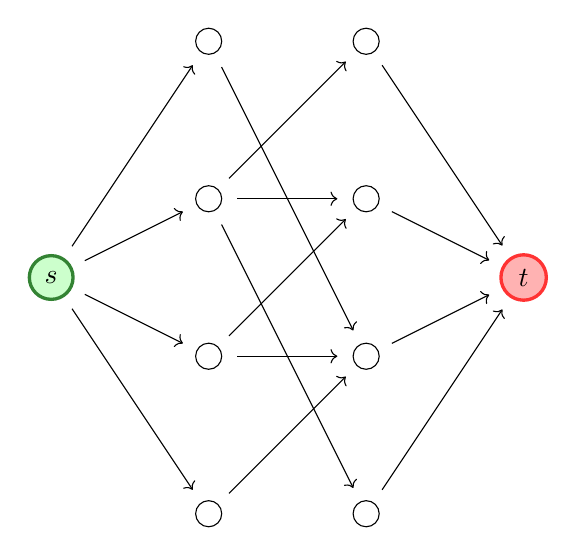
\begin{tikzpicture}
      \node[main] (1) at (0, 0) {};
      \node[main] (2) at (0, -2) {};
      \node[main] (3) at (0, -4) {};
      \node[main] (4) at (0, -6) {};

      \node[main] (5) at (2, 0)  {};
      \node[main] (6) at (2, -2) {};
      \node[main] (7) at (2, -4) {};
      \node[main] (8) at (2, -6) {};

      \draw [->] (1) -- (7);
      \draw [->] (2) -- (6);
      \draw [->] (3) -- (7);
      \draw [->] (4) -- (7);
      \draw [->] (2) -- (5);
      \draw [->] (3) -- (6);
      \draw [->] (2) -- (8);

      \node[main, source] (s) at (-2, -3) {$s$};
      \node[main, sink] (t) at (4, -3) {$t$};

      \draw [->] (s) -- (1);
      \draw [->] (s) -- (2);
      \draw [->] (s) -- (3);
      \draw [->] (s) -- (4);

      \draw [<-] (t) -- (5);
      \draw [<-] (t) -- (6);
      \draw [<-] (t) -- (7);
      \draw [<-] (t) -- (8);
    \end{tikzpicture}
  \end{center}

  Then, finding the maximum flow on this network is analogous to finding a
  maximum matching.

  \note {
    We need to reassert that all flows here are integers values, if they did
    not, our Ford-Fulkerson algorithm may not be able to find the optimal
    flow.
  }

  Let's look at another example.

  \example {
    Consider the $2 \times 2$ complete bipartite graph.

    \begin{center}
      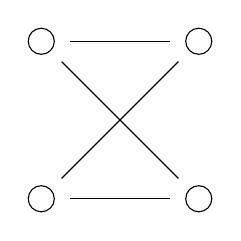
\begin{tikzpicture}
        \node[main] (1) at (0, 0) {};
        \node[main] (2) at (0, -2) {};
        \node[main] (3) at (2, 0) {};
        \node[main] (4) at (2, -2) {};

        \draw [-] (1) -- (3);
        \draw [-] (1) -- (4);
        \draw [-] (2) -- (3);
        \draw [-] (2) -- (4);

        % \node[main, source] (s) at (-2, -1) {$s$};
        % \node[main, sink] (t) at (4, -1) {$t$};
        %
        % \draw [->] (s) -- (1);
        % \draw [->] (s) -- (2);
        %
        % \draw [->] (3) -- (t);
        % \draw [->] (4) -- (t);
      \end{tikzpicture}
    \end{center}

    Suppose all edges have unit capacities, then we can send the following
    flows.

    \begin{center}
      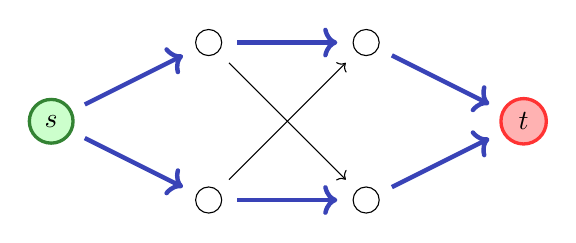
\begin{tikzpicture}
        \node[main] (1) at (0, 0) {};
        \node[main] (2) at (0, -2) {};
        \node[main] (3) at (2, 0) {};
        \node[main] (4) at (2, -2) {};

        \draw [->, selected] (1) -- (3);
        \draw [->] (1) -- (4);
        \draw [->] (2) -- (3);
        \draw [->, selected] (2) -- (4);

        \node[main, source] (s) at (-2, -1) {$s$};
        \node[main, sink] (t) at (4, -1) {$t$};

        \draw [->, selected] (s) -- (1);
        \draw [->, selected] (s) -- (2);

        \draw [->, selected] (3) -- (t);
        \draw [->, selected] (4) -- (t);
      \end{tikzpicture}
    \end{center}

    or

    \begin{center}
      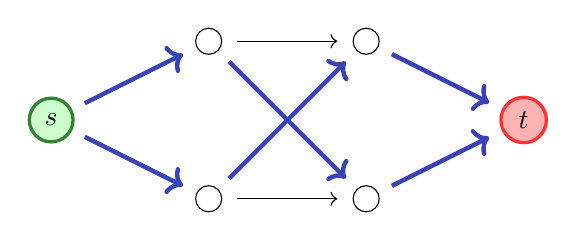
\begin{tikzpicture}
        \node[main] (1) at (0, 0) {};
        \node[main] (2) at (0, -2) {};
        \node[main] (3) at (2, 0) {};
        \node[main] (4) at (2, -2) {};

        \draw [->] (1) -- (3);
        \draw [->, selected] (1) -- (4);
        \draw [->, selected] (2) -- (3);
        \draw [->] (2) -- (4);

        \node[main, source] (s) at (-2, -1) {$s$};
        \node[main, sink] (t) at (4, -1) {$t$};

        \draw [->, selected] (s) -- (1);
        \draw [->, selected] (s) -- (2);

        \draw [->, selected] (3) -- (t);
        \draw [->, selected] (4) -- (t);
      \end{tikzpicture}
    \end{center}

    Both of these correspond to a maximum matching.
  }

  Let's prove that this always works.

  \Lemma {
    The size of a max matching in given bipartite graph equals the value of a
    max flow in the corresponding flow network.
  }
  {
    $\Rightarrow$ \underline{Given a Matching, we can construct a Flow}

    Given a matching $M$, construct a flow by sending $1$ unit of flow for
    each corresponding edge in the flow network.

    We also send $1$ unit of flow from $s$ to every matched vertex in $A$, and
    $1$ unit of flow for each matched vertex in $B$ to $t$.

    This is a valid flow, and the value of this flow is the size of the
    matching $|M|$.

    $\Leftarrow$ \underline{Given a Flow, we can construct a Matching}

    If there exists a (maximum) flow of value $k$, then there exists an
    integer-valued flow of value $k$ (This is because we have integer-valued
    capacities, so Ford-Fulkerson will find such a flow).

    Since there can be at most one unit of flow into each vertex in $A$ (by
    the structure of the flow network), each edge from $A$ to $B$ can have at
    most one unit of flow.

    Consider the cut ($\{s\} \cup A$, $\{t\} \cup B$), the flow leaving the
    cut is $k$, and there must be $k$ edges carrying the flow from $A$ to $B$.

    Let $M$ be the set of edges from $A$ to $B$ that carry flow. Since we have
    one unit of flow on all edges, none of the edges are shared (that's the
    conservation constraint)

    Therefore $M$ must be a matching.
  }

  Great! Now we have a way to find a maximum matching. Let's quickly look at
  the running time.

  \subsubsection{Running Time}

  Suppose $|A| = |B| = n$. Let $C$ be the total capacity of the edges leaving
  $s$, then $C = n$.

  The Ford-Fulkerson running time is $\O(n(m + n))$

  \subsection{Extensions to the Max Flow Problem}

  These are alternative variants to the problems we've seen thus far. We're
  not doing anything new here, but it will give us helpful notions to solve
  network flow problems.

  \subsubsection{Multiple Sources and Sinks}

  \btw {
    Suppose that we have multiple sources and sinks. These nodes still behave
    as they used to before, but this time we may have more than one of each.

    In this case, we say that the flow is the sum of the flow into each sink.
  }

  Consider the following graph

  \begin{center}
    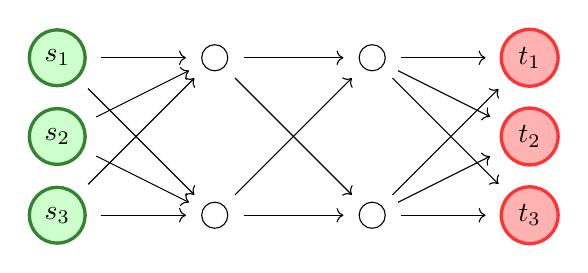
\begin{tikzpicture}
      \node[main] (1) at (0, 0) {};
      \node[main] (2) at (0, -2) {};
      \node[main] (3) at (2, 0) {};
      \node[main] (4) at (2, -2) {};

      \draw [->] (1) -- (3);
      \draw [->] (1) -- (4);
      \draw [->] (2) -- (3);
      \draw [->] (2) -- (4);

      \node[main, source] (s1) at (-2, 0) {$s_1$};
      \node[main, source] (s2) at (-2, -1) {$s_2$};
      \node[main, source] (s3) at (-2, -2) {$s_3$};

      \node[main, sink] (t1) at (4, 0) {$t_1$};
      \node[main, sink] (t2) at (4, -1) {$t_2$};
      \node[main, sink] (t3) at (4, -2) {$t_3$};

      \draw [->] (s1) -- (1);
      \draw [->] (s1) -- (2);
      \draw [->] (s2) -- (1);
      \draw [->] (s2) -- (2);
      \draw [->] (s3) -- (1);
      \draw [->] (s3) -- (2);

      \draw [->] (3) -- (t1);
      \draw [->] (4) -- (t1);
      \draw [->] (3) -- (t2);
      \draw [->] (4) -- (t2);
      \draw [->] (3) -- (t3);
      \draw [->] (4) -- (t3);
    \end{tikzpicture}
  \end{center}

  We can reduce this to the problem we already know how to solve.

  \begin{center}
    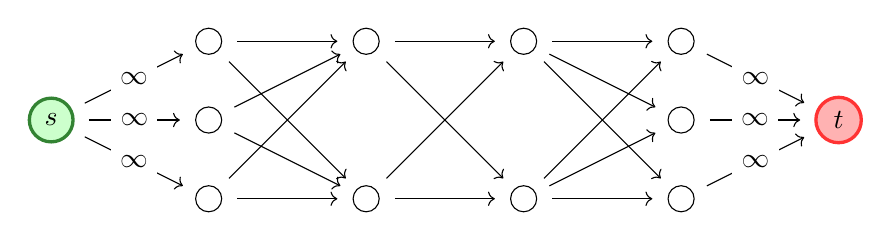
\begin{tikzpicture}
      \node[main] (1) at (0, 0) {};
      \node[main] (2) at (0, -2) {};
      \node[main] (3) at (2, 0) {};
      \node[main] (4) at (2, -2) {};

      \draw [->] (1) -- (3);
      \draw [->] (1) -- (4);
      \draw [->] (2) -- (3);
      \draw [->] (2) -- (4);

      \node[main, source] (s) at (-4, -1) {$s$};
      \node[main, sink] (t) at (6, -1) {$t$};

      \node[main] (5) at (-2, 0) {};
      \node[main] (6) at (-2, -1) {};
      \node[main] (7) at (-2, -2) {};

      \node[main] (8) at (4, 0) {};
      \node[main] (9) at (4, -1) {};
      \node[main] (10) at (4, -2) {};

      \draw [->] (5) -- (1);
      \draw [->] (5) -- (2);
      \draw [->] (6) -- (1);
      \draw [->] (6) -- (2);
      \draw [->] (7) -- (1);
      \draw [->] (7) -- (2);

      \draw [->] (3) -- (8);
      \draw [->] (4) -- (8);
      \draw [->] (3) -- (9);
      \draw [->] (4) -- (9);
      \draw [->] (3) -- (10);
      \draw [->] (4) -- (10);

      \draw [->] (s) -- node[mid] {$\infty$} (5);
      \draw [->] (s) -- node[mid] {$\infty$} (6);
      \draw [->] (s) -- node[mid] {$\infty$} (7);

      \draw [->] (8) -- node[mid] {$\infty$} (t);
      \draw [->] (9) -- node[mid] {$\infty$} (t);
      \draw [->] (10) -- node[mid] {$\infty$} (t);
    \end{tikzpicture}
  \end{center}

  You can convince yourself that these graphs represent the same thing.

  \subsubsection{Circulations with Demands}

  Given a flow network $G = (V, E)$ with edge capacities. Now each vertex has
  a {\bf demand} $d_v$.

  \begin{itemize}
    \item If $d_v > 0$, it means that $v$ is a net sink and should receive $d_v$
      {\it more} units of flow that it outputs.
    \item If $d_v < 0$, it means that $v$ is a new source and should supply
      $-d_v$ more units of flow that it takes in.
  \end{itemize}

  \note {
    If $d_v = 0$, this is just a vertex which conserves flow, which is exactly
    the vertices that we've been working with up to this point.
  }

  \begin{itemize}
    \item Let $S$ be the set of vertices $v \in V$ with negative demands $d_v < 0$
    \item Let $T$ be the set of vertices with positive demands $d_v > 0$.
  \end{itemize}

  \Definition {Circulation} {
    A {\bf circulation} is a function $f: E \to \R^+$ satisfying

    \begin{enumerate}
      \item \underline{Capacity Conditions}

        \[
          (\forall e \in E) [0 \le f(e) \le C_e]
        \]

        Where $C_e$ is the capacity of edge $e$.

      \item \underline{Demands Conditions}

        \[
          (\forall v \in V)[f^\text{in}(v) - f^\text{out}(v) = d_v]
        \]

        In other words, the {\it demand} of $v$ is exactly the difference
        between the flow going in, and the flow going out.
    \end{enumerate}
  }

  Notice that up to this point, we've been thinking about {\it maximization}
  problems. Here, there is nothing to maximize. We only want to know {\it if}
  this is feasible.

  Let's take a look at a simple example.

  \example {
    Suppose we have the following network.

    \begin{center}
      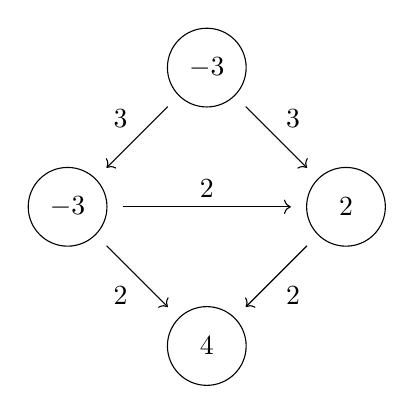
\begin{tikzpicture}[
          main/.style = {draw, circle, outer sep=2mm, minimum size=10mm},
        ]
        \node[main] (t) {$-3$};
        \node[main] (l) [below left of=t] {$-3$};
        \node[main] (b) [below right of=l] {$4$};
        \node[main] (r) [below right of=t] {$2$};

        \draw [->] (t) -- node[above left] {$3$} (l);
        \draw [->] (t) -- node[above right] {$3$} (r);
        \draw [->] (l) -- node[above] {$2$} (r);
        \draw [->] (l) -- node[below left] {$2$} (b);
        \draw [->] (r) -- node[below right] {$2$} (b);
      \end{tikzpicture}
    \end{center}

    Here, the numbers inside the nodes represent the demands. For the top
    node, the demand is $-3$, so it must {\it supply exactly} $3$ units of flow.

    The numbers on the edges haven't changed. They represent the maximum
    capacities that can be sent on that edge.

    {\bf Question}: Is this a feasible circulation problem? Can we find a flow
    value for every edge so that we satisfy the demands of all vertices?

    {\bf Answer}: Yes!

    \begin{center}
      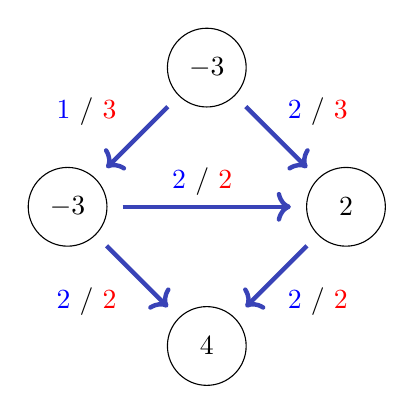
\begin{tikzpicture}[
          main/.style = {draw, circle, outer sep=2mm, minimum size=10mm},
        ]
        \node[main] (t) {$-3$};
        \node[main] (l) [below left of=t] {$-3$};
        \node[main] (b) [below right of=l] {$4$};
        \node[main] (r) [below right of=t] {$2$};

        \draw [->, selected] (t) -- node[above left] {\fc{1}{3}} (l);
        \draw [->, selected] (t) -- node[above right] {\fc{2}{3}} (r);
        \draw [->, selected] (l) -- node[above] {\fc{2}{2}} (r);
        \draw [->, selected] (l) -- node[below left] {\fc{2}{2}} (b);
        \draw [->, selected] (r) -- node[below right] {\fc{2}{2}} (b);
      \end{tikzpicture}
    \end{center}

    We'll see exactly how to get this answer.
  }

  Firstly, notice that the sum of all the demands better be zero.

  \[
    \sum_{v \in V} d_v = \sum_{v \in V} \left(f^\text{in}(v) - f^\text{out}(v)\right) = 0
  \]

  This should make sense: the demand constraint say that the total amount of
  stuff going in must be the total amount of stuff going out. 

  However, if the sum {\it is} zero, that doesn't necessarily mean that the
  demands are feasible. In other words, the condition is not sufficient.

  {\bf Goal}: We want to find a reduction to a standard max flow problem.

  We want to construct a graph $G'$, here's how. 

  \begin{enumerate}
    \item We add a source $s^*$ and a sink $t^*$ to $G'$.

    \item We add all the edges between vertices of $G$, and keep their
      capacities the same.

    \item For all the vertices $v \in S$ (the vertices with negative demand,
      these are the vertices that {\it output more} than they take in), we add
      an edge $(s^*, v)$ of capacity $-d_v$.

      In other words, $s^*$ is going to provide the necessary 
      flow that $v$ demands.

      It's important to notice that $-d_v$ is positive here, because $d_v$ is
      negative. After all, that's what it means to be a source vertex.

    \item For all the vertices $v \in T$ (the vertices with positive demand,
      these are the vertices that {\it take in more} than they output), we add
      an edge $(v, t^*)$ of capacity $+d_v$.
  \end{enumerate}

  In this network $G'$, we would like it to be the case that the maximum flow
  has {\it something} to do with the feasibility problem in $G$. How can we
  tell whether this is the case?

  Of course, the max flow problem is always feasible: just take the zero flow.
  But how can $G'$ help us solve our satisfiability problem for $G$?

  {\bf Answer}: If we can completely saturate $G'$, then $G$ is feasible.

  Let $D$ be the sum of all demands of $T$, the ``sink-like" vertices.

  \[
    D = \sum_{v \in T} d_v
  \]

  We saw earlier that the net demands must be zero, so we have that

  \[
    D = \sum_{v \in T} d_v = - \sum_{v \in S} d_v
  \]

  \Theorem {
    There is a feasible circulation with demands $\{d_v\}$ {\bf if and only
    if} the max $s^* - t^*$ flow in $G'$ has value $D$.

    If all capacities and demands are integers, and the circulation demands
    are feasible (i.e. net demand is zero), then the circulation can be chosen
    to be integer values.

    (There can actually be several solutions, but any of them is fine for our
    purposes.)
  }
  {
    Clearly, the max flow cannot exceed $D$, since

    \[
      \sum_{e \text{ out of } s^*} C_e = D
    \]

    (in other words, the sum of all the stuff coming out of the source vertex
    is $D$)

    If there exists a feasible circulation in $G$, we can construct a flow in
    $G'$ by sending flow $-d_v$ on edges $(s^*, v)$, and flow $d_v$ on edges
    $(v, t^*)$.

    This is an $s^* - t^*$ flow in $G'$ of value $D$.

    If there exists a flow $G'$ of value $D$, every edge out of $s^*$ and into
    $t^*$ must saturate its capacity, so we can delete those edges to get a
    circulation $f$ in $G$ that satisfies the demand condition from earlier

    \[
      f^\text{in} - f^\text{out} = d_v
    \]

    for all vertices $v$ of $G$.

    Since the max flow in $G'$ can be integer-valued, there exists an
    integer-valued circulation.
  }

  \subsubsection{Lower bounds on an Edge}

  Suppose we also impose a constraint that the flow on edge $e$ must be at
  least $l_e$. For all edges of the flow network, $l_e \le f(e) \le c_e$.

  (Our demand conditions are still the same.)

  Again, we're going to reduce this to something we can solve.

  Start from an initial ``circulation" with $f_0(e) = l_e$. In other words, we
  start with the minimum amount of flow. This satisfies the capacity
  conditions since $l_e \le c_e$, but in general, it won't satisfy the demand
  conditions.

  Recall what the demand conditions were, for all vertices in $G$

  \[
    f_0^\text{in}(v) - f_0^\text{out}(v)
  \]

  but we initialized every vertex as having the minimum flow allowed! So we
  actually have

  \begin{align*}
    &f_0^\text{in}(v) - f_0^\text{out}(v) \\
    =&\sum_{e \text{ into } v} l_e - \sum_{e \text{ out of } v} l_e
  \end{align*}

  Let's define $L_v$ to be this value.

  \[
    L_v := \sum_{e \text{ into } v} l_e - \sum_{e \text{ out of } v} l_e
  \]

  Ideally, we want to meet all the demands, so we would need $L_v$ to equal
  $d_v$ for all vertices $v$ in our graph. But recall that we picked the flows
  to be the minimum values possible. How convenient! We can only go up from
  here.

  We want to add a flow $f_1$ that makes up the rest of the demand (i.e. $d_v -
  L_v$)

  \[
    f_1^\text{in}(v) - f_1^\text{out}(v) = d_v - L_v
  \]

  In other words, we want to add {\it that} much flow to each vertex $v$, using
  the remaining capacity $c_e - l_e$ on all edges $e$.

  This is starting to sound like a demand problem.

  We construct a circulation with demands problem on the same graph with new
  capacities $c_e - l_e$, and new demands $d_v - L_v$.

  Let's prove that this actually works.

  \Theorem {
    There is a feasible circulation in the circulation with demands and lower
    bounds problem {\bf if and only if} there is a feasible solution in
    corresponding circulation with demands problem.

    If all demands, capacities, and lower bounds are integers (and the problem
    is feasible), then there is an integer-valued solution.
  }
  {
    Suppose there exists a circulation $f'$ in the problem without lower bounds.
    Let $f(e) = f'(e) + l_e$.

    This clearly satisfies the capacity conditions, and

    \begin{align*}
      f^\text{in}(v) - f^\text{out}(v) =&\sum_{e \text{ into } v} (f'(e) + l_e)
      - \sum_{e \text{ out of } v} (f'(e) + l_e) \\
      =&L_v + d_v - L_v \\
      =&d_v
    \end{align*}

    So this satisfies the demand conditions.

    Conversely, suppose there exists a circulation $f$ in the original problem.
    Let $f'(e) = f(e) - l_e$.

    Then $f'$ satisfies the capacity conditions, and

    \begin{align*}
      f^{'\text{in}}(v) - f^{'\text{out}}(v) =&\sum_{e \text{ into } v} (f(e) - l_e) - \sum_{e \text{ out of } v} (f(e) - l_e) \\
    \end{align*}

    so it satisfies the demand conditions in the network without lower bounds.
  }

  \newpage
  \section{Reductions}

  To show that problem $X$ is {\it at least} as hard as $Y$, we can give a
  {\bf reduction} from $Y$ to $X$. A procedure that solves $Y$ using the ability
  to solve $X$.

  To have this quantify efficiency, we want to the procedure to be efficient.

  \Definition {Poly-time Reducibility}
  {
    If any instance of $Y$ can be solved by a polynomial time algorithm that can
    make polynomially many calls to a procedure for solving instances of $X$,
    then we say that $Y$ is {\bf poly-time reducible} to $X$, and we write $Y
    \le_{p} X$.
  }

  \example {
    We showed that the Bipartite-Matching problem could be reduced to the Max
    Flow problem.

    \[
      \text{Bipartite Matching} \le_p \text{Max Flow}
    \]
  }

  Let's take a look at some example problems.

  \subsection{Independent Set Problem}

  \Definition {Independent Set}
  {
    An {\bf Independent Set} in a graph is a subset of vertices, no two of which
    are adjacent.
  }

  The Maximum Independent set problem asks us to find the largest independent
  set in a graph.

  % \note {
  %   It will be helpful to have yes/no algorithms for search
  % }

  Let's do an example.

  \example {
    Suppose we have the following graph $G$.

    \begin{center}
      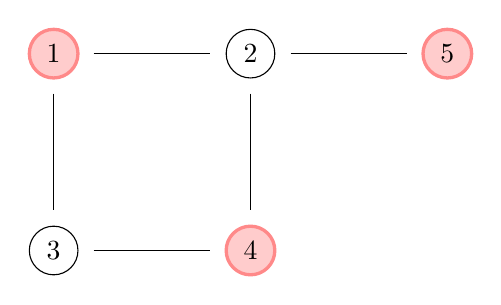
\begin{tikzpicture}
        \node[main, draw=darkred!80, fill=red!20, very thick] (1) {$1$};
        \node[main] (3) [below of=1] {$3$};
        \node[main] (2) [right of=1] {$2$};
        \node[main, draw=darkred!80, fill=red!20, very thick] (4) [below of=2] {$4$};
        \node[main, draw=darkred!80, fill=red!20, very thick] (5) [right of=2] {$5$};

        \draw [-] (1) -- (3);
        \draw [-] (1) -- (2);
        \draw [-] (3) -- (4);
        \draw [-] (2) -- (4);
        \draw [-] (2) -- (5);
      \end{tikzpicture}
    \end{center}
  }

  \subsection{Vertex Cover Problem}

  \Definition {Vertex Cover}
  {
    A {\bf Vertex Cover} of a graph is a subset of vertices such that every edge
    has at least one end in that subset.
  }

  The vertex cover problem asks to find a {\it smallest} vertex cover.

  % \section{NP and NP-Completeness}

  \example {
    A minimal vertex cover of this graph would be

    \begin{center}
      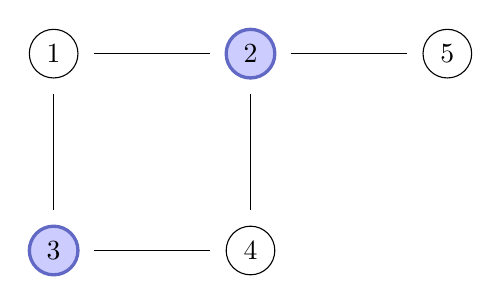
\begin{tikzpicture}
        \node[main] (1) {$1$};
        \node[main, draw=darkblue!80, fill=blue!20, very thick] (3) [below of=1] {$3$};
        \node[main, draw=darkblue!80, fill=blue!20, very thick] (2) [right of=1] {$2$};
        \node[main] (4) [below of=2] {$4$};
        \node[main] (5) [right of=2] {$5$};

        \draw [-] (1) -- (3);
        \draw [-] (1) -- (2);
        \draw [-] (3) -- (4);
        \draw [-] (2) -- (4);
        \draw [-] (2) -- (5);
      \end{tikzpicture}
    \end{center}
  }

  This problems are actually inverses of each other! The smallest vertex cover
  will produce the largest independent set.

  \Lemma {
    For any graph $G = (V, E)$, a vertex subset $S \subseteq V$ is an
    independent set {\bf if and only if} $V \setminus S$ is a vertex cover.
  }
  {
    $\Rightarrow$

    Suppose $S$ is an independent set. Then for any $\{u, v\} \in E$, at most
    one of $u, v$ is in $S$, so {\it at least one} is in $V \setminus S$, so $V
    \setminus S$ is a vertex cover by definition of a vertex cover.

    $\Leftarrow$

    Suppose $V \setminus S$ is a vertex cover. Suppose for the sake of
    contradiction that $u \in S$ and $v \in S$, and $\{u, v\} \in E$. Then
    neither end of $E$ would be in $V \setminus S$, so that edge is not covered
    and $V \setminus S$ is not a cover. This is a contradiction, so $S$ is an
    independent set.
  }

  \note {
    This is a special example! In most cases, things will only reduce in one
    direction.
  }

  What this shows is that the Independent Set problem is polynomial time
  reducible to the Vertex Cover problem, and vice versa.

  \subsection{Set Cover Problem}

  Suppose that we're given a set $U$ and subsets $S_1, S_2, \dots, S_m \subseteq
  U$. We want to find a minimal subset of the $S_i$s so that the union is all of
  $U$.

  % Let's do an example.

  % \example {
  %   Suppose we have the sets
  % }

  \Theorem {
    Set Cover is {\it at least} as hard as Vertex Cover.

    \[
      \text{Vertex Cover} \le_p \text{Set Cover}
    \]
  }
  {
    Given an instance of Vertex Cover, a graph $G = (V, E)$, we want to
    construct an instance of Set Cover.

    Let $U = E$. For all $v \in V$, let $S_v$ be the set of edges incident of
    $v$.

    {\bf Claim}: $G$ can be covered with $k$ vertices {\bf if and only if} $U$
    can be covered with $k$ $S_v$s.

    \begin{itemize}
      \item If $\{v_1, \dots, v_k\}$ is a vertex cover, then $\{S_{v_1}, \dots,
        S_{v_k}\}$ include all the edges.

      \item If $\{S_{v_1}, \dots, S_{v_k}\}$ include all the edges, then $\{v_1,
        \dots, v_k\}$ is a vertex cover, by definition.
    \end{itemize}
  }

  By solving the set cover problem, we will solve the original vertex cover
  problem.

  \subsection{Boolean Satisfiability}

  \Definition {} {
    Given a set of Boolean variables $\{x_1, \dots, x_n\}$, a {\bf term} or {\bf
    literal} is $x_i$ or $\bar x_i$.

    A {\bf Clause} is a {\it disjunction} of terms.

    \[
      (x_2 \vee x_6 \vee \bar x_{11})
    \]

    We say that a set of clauses is {\bf satisfiable} if there is an assignment
    of the $x_i$s to True/False so that all clauses evaluate to True.
  }

  The Boolean Satisfiability Problem (SAT) asks whether a given set of clauses
  is satisfiable.

  \note {
    We never repeat a variable (or its negation), inside of any clause.
  }

  \note {
    $k$-SAT is a subset of SAT where each clause has exactly $k$ terms.
  }

  In 3-SAT, each clause has exactly 3 terms.

  \Theorem {
    3-SAT is no harder than the Independent Set Problem.

    \[
      \text{$3$-SAT} \le_p \text{Independent Set}
    \]
  }
  {
    Given a 3-SAT instance, we use ``gadgets" to construct a graph that has a
    ``big" independent set {\bf if and only if} 3-SAT is satisfiable.

    For a clause $C_j$, we introduce 3 vertices $v_{j, 1}, v_{l, 2}, v_{j, 3}$
    and we connect them with a triangle.

    We also connect $v_{j, l}$ and $v_{j', l'}$ if term $l$ in $C_j$ is the
    negation of term $l'$ in $C_j'$.

    \example {
      \[
        (x_1 \vee x_2 \vee \bar x_3) \wedge (\bar x_1 \vee x_2 \vee x_4)
      \]

      \TODO{} add triangle picture, Apr. 20 15:13
    }

    {\bf Claim}: The formula is satisfiable {\bf if and only if} this graph 
    has an independent set of size $m$ for $m$ clauses.

    {\bf Proof}: If the formula is satisfiable for every clause, there must be
    some variable setting that shows the clause is true. (There must be at least
    one variable in each clause that makes that clause true.) We'll take this
    variable as the vertex that we'll keep in the independent set problem.

    This gives a set of vertices of size equal to the number of triangles. It's
    independent because 

    \begin{itemize}
      \item We only take one vertex per triangle
      \item We don't pick vertices at both ends of an edge between triangles.
    \end{itemize}

    \note {
      We have one triangle for every clause, that's how we create the triangles.
    }

    Conversely, there is an independent set of size equal to the number of
    triangles. It must have one vertex per triangle. Construct a satisfying
    assignment by setting the corresponding variables to the values that make
    those clauses true. Since an independent set can't contain vertices from
    different triangles corresponding to variables $x_i$ and $\bar x_i$, this
    assignment will be consistent. It makes every clause evaluate to true, so it
    satisfies the formula.
  }

  We've now shown that 3-SAT is the easiest of these problems that we've looked
  at. It's no harder than Independent Set, which is no harder than Vertex
  Cover, which is no harder than Set Cover

  \[
    \text{3-SAT} \le_p \text{Independent Set} =_p \text{Vertex Cover} \le_p
    \text{Set Cover}
  \]

  \section{NP and NP-Completeness}

  We say that an algorithm is sufficient if it runs in time polynomial in the
  input size. We can collect these problems with efficient solutions into a {\bf
  complexity class} called $P$.

  We'll focus on decision problems: problem for which we can give a yes/no
  answer. Characterize such problem by a {\bf language} $L \subseteq \Sigma^*$,
  the set of all possible inputs. $L$ contains only the set of instances for
  which the answer to the problem is Yes.

  A language $L$ is in $P$ if there exists an algorithm running in time
  polynomial in $n$ that accepts $x \in \Sigma^n$ if $x \in L$, and rejects $x
  \in \Sigma^n$ if $x \not\in L$.

  \example {
    For 3-SAT, $x$ is a set of clauses, $L$ is the set of satisfiable 3-SAT
    clauses.
  }

  The harder problems that we've considered (i.e. 3-SAT) may not have efficient
  algorithms, but they all have the property that solutions can be verified
  efficiently.

  \example {
    \begin{itemize}
      \item For 3-SAT, the satisfying assignment can be checked very quickly.
      \item For the independent set problem, its very quick to check whether the
        vertices of the independent set  are really independent.
    \end{itemize}
  }

  The class $NP$ is the set of problems whose yes instances can be efficiently
  verified.

  \example {
    If an instance $x$ is in the language $L$, then there must exist a witness
    (a proof) $y$, and some polynomial time algorithm $A$, that you can run on
    input $x$ and $y$, and it should accept.

    \[
      x \in L \Rightarrow \exists y, A(x, y) \text{ accepts}
    \]

    Conversely, if there is input $x$ to the algorithm, for any proof $y$ they
    try to give you, you will not be fooled.

    \[
      x \not\in L \Rightarrow \forall y, A(x, y) \text{ rejects}
    \]
  }

  Clearly, $P \subseteq NP$, $P$ is the set problems that are quick to solve and
  quick to check, and $NP$ is the set of problems that are hard to solve but
  quick to check.

  We can get evidence for the hardness of $NP$ problems using reductions.

  \Definition {NP Hard}
  {
    If, for all problems $y$ that are in $NP$, $Y \le_p X$ ($X$ is at least as
    hard as $Y$), we say that $X$ is NP hard.
  }

  \Definition {NP Complete}
  {
    If $X$ is in $NP$, and $X$ is NP Hard, we say that $X$ is $NP$ complete.
  }

  \subsection{Trivial NP-Complete Problem: Circuit Satisfiability}

  A {\bf circuit} is a labeled DAG where sources (the vertices with no incoming
  edges) are going to be labeled either $0$, $1$ or \texttt{free} (meaning you
  figure out how to set them.)

  We have vertices with both incoming and outgoing edges, these correspond to
  boolean logic gates (\texttt{AND} / \texttt{OR} / \texttt{NOT} gates.)

  There is a unique sink (a vertex with no outgoing edges) which represents the
  output.

  {\bf Problem}: Is there an assignment of the \texttt{free} inputs that makes
  the circuit evaluate to $1$?


  \NamedTheorem{
    \subsection{Cook-Levin Theorem}
  }
  {
    $3$-SAT is $NP$-Complete.
  }
  {
    3-SAT is in NP since we can provide a satisfying assignment as the proof.
    This can be efficiently verified by checking that each clause evaluates to
    true. Since the problem is easy to check, it's in NP.

    Now to show that it's in NP-Hard. Given any instance of circuit SAT, we
    construct an instance of 3-SAT (we must be able to construct this in
    polynomial time) such that, if one is satisfiable if and only if the other
    is. We essentially want to translate Circuit Sat to 3-SAT.

    We introduce a boolean variable $x_v$ for every vertex $v$ of the circuit.

    {\texttt{NOT}}

    \begin{center}
      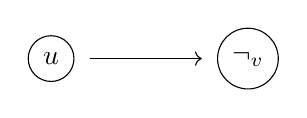
\begin{tikzpicture}
        \node[main] (u) {$u$};
        \node[main] (v) [right of=u] {$\neg_v$};

        \draw [->] (u) -- (v);
      \end{tikzpicture}
    \end{center}

    Add clauses

    \[
      (x_u \vee x_v) \wedge (\bar x_u \vee \bar x_v)
    \]

    (note that this is 2-SAT, but that's alright, 2-SAT is easier than 3-SAT)

    {\texttt{OR}}

    \begin{center}
      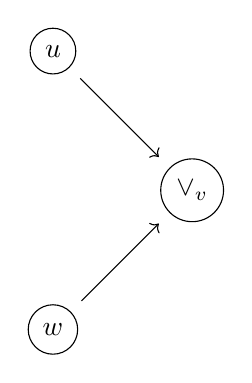
\begin{tikzpicture}
        \node[main] (u) {$u$};
        \node[main] (v) [below right of=u] {$\vee_v$};
        \node[main] (w) [below left of=v] {$w$};

        \draw [->] (u) -- (v);
        \draw [->] (w) -- (v);
      \end{tikzpicture}
    \end{center}

    Add clauses

    \[
      (x_v \vee \bar x_u) \wedge (x_v \vee \bar x_w) \wedge (\bar x_v \vee x_u
      \vee x_w)
    \]

    {\texttt{AND}}

    Simply use DeMorgan's Law on the above.

    \begin{center}
      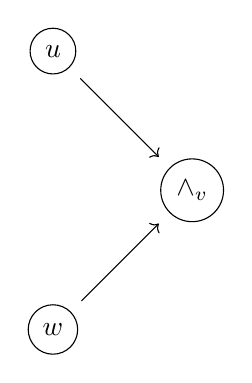
\begin{tikzpicture}
        \node[main] (u) {$u$};
        \node[main] (v) [below right of=u] {$\wedge_v$};
        \node[main] (w) [below left of=v] {$w$};

        \draw [->] (u) -- (v);
        \draw [->] (w) -- (v);
      \end{tikzpicture}
    \end{center}

    Add clauses

    \[
      (x_v \vee \bar x_u \vee \bar x_w) \wedge (\bar x_v \vee x_u) \wedge (\bar
      x_v \vee x_w)
    \]

    If we have a \texttt{0} input, we want to include a clause that forces this
    to be a zero, just add $\bar x_v$. Conversely for a \texttt{1}, we want to
    add $x_v$.

    For a \texttt{free} input, we just add nothing.

    For the output, $x_v$ will evaluate to true if and only if the circuit
    evaluates to true.

    To make this a 3-SAT formula, we add some variables (4 of them)

    \[
      z_1, z_2, z_3, z_4
    \]

    with clauses

    \[
      (\bar z_i \vee z_3 \vee z_4) \wedge (\bar z_i \vee z_3 \vee \bar
      z_4) \wedge (\bar z_i \vee \bar z_3 \vee z_4) \wedge (\bar z_i \vee \bar z_3
      \vee \bar z_4)
    \]

    The only way to satisfy this is for $z_i$ to be 0. We add this for $i = 1,
    2$ so that $z_1 = z_2 = 0$ in any satisfying assignment.

    Then we can pad clauses to have exactly 3 terms.

    \[
      x_v \Rightarrow (x_v \vee z_1 \vee z_2)
    \]
  }

  \subsection{Other NP-Complete Problems}

  \subsubsection{The Traveling Salesman Problem}

  Given cities $v_1, \dots, v_n$, distances $d(v_i, v_j)$ and a bound $D$, is
  there a tour of the cities of total length at most $D$?

  \subsubsection{The Hamiltonian Cycle Problem}

  Given a graph, is there a cycle in the graph that visits every vertex exactly
  once?

  \subsubsection{The 3 Dimensional Matching Problem}

  Given some disjoint sets $X, Y, Z$, each of size $n$. We're also given a set
  $T \subset X \times Y \times Z$ of ordered triples.

  Is there a set of triples so that every element of $X \cup Y \cup Z$ is
  included in exactly one triple?

  \subsubsection{The 3-Coloring Problem}

  Can we assign 3 colors to the vertices of a graph so that no two adjacent
  vertices have the same color?

  \subsubsection{The Subset Sum Problem}

  Given numbers $w_1, \dots, w_n$, and a target value $W$ (all positive.)

  Is there a subset of the $w_i$s that sum to exactly $W$?

  \subsubsection{Scheduling with least times and deadlines}

  Given $n$ jobs, indexed by some $1 \le i \le n$. Every job has some release
  time $r_i$: you cannot start that job before $r_i$, it has some deadline
  $d_i$, and some time $t_i$.

  Job $i$ must be scheduled for duration $t_i$, starting after $r_i$, and ending
  before $d_i$.

  Given a list of job, is such a schedule possible?

  \subsection{The Hamiltonian Cycle Problem}

  \Definition{The Hamiltonian Cycle Problem}
  {
    Given a directed (or undirected, that works too) $G = (V, E)$, a {\bf
    Hamiltonian Cycle} is a cycle that visits each vertex exactly once.
  }

  Definitely not every graph has such a cycle. Let's look at an example

  \example {
    \begin{center}
      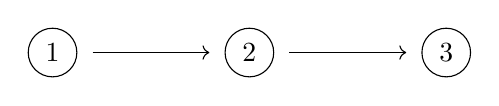
\begin{tikzpicture}
        \node[main] (1) {1};
        \node[main] (2) [right of=1] {2};
        \node[main] (3) [right of=2] {3};

        \draw [->] (1) -- (2);
        \draw [->] (2) -- (3);
      \end{tikzpicture}
    \end{center}

    Here, you can go from 1, to 2, to 3, but you can't go back to 1.
  }

  \sidenote{
    Homework Deadline extended to Friday May 5
  }

  \subsubsection{Showing NP Completeness}

  \Theorem {
    Hamiltonian Cycle is NP-Complete.
  }
  {
    Again, we have to show two things:

    \begin{enumerate}
      \item The problem is in NP, so it can be verified efficiently
      \item The problem is in NP Hard, so its at least as hard as all the
        problems in NP.
    \end{enumerate}

    {\bf The problem is in NP}.

    The proof is a list of all vertices . The verifier checks that every
    adjacent pair of vertices is joined by an edge, including the last vertex to
    the first. It also checks that each vertex appears in the list exactly once.

    These checks take polynomial time and accepts if and only if the list
    truly specifies a Hamiltonian path.

    {\bf The problem is NP-Hard}

    3-SAT is often a good fallback choice if we don't know where to start from,
    this is exactly what we're going to do here. It doesn't seem like these
    problems have all that much in common, but in fact they do.

    Remember the direction of the reduction here: we want to take an instance of
    3-SAT, and construct a graph that corresponds to that 3-SAT formula.

    Given a 3-SAT formula with variables $\{x_1, \dots, x_n\}$, we construct a
    graph with ``long" paths $\{P_1, \dots, P_n\}$, in one to one correspondence
    with $x_1, \dots, x_n$. We also add vertices $s, t$ connected as follows.

    \TODO{} draw graph from class (Tue May 2, 14:23)
    % \begin{center}
    %   \begin{tikzpicture}
    %     \node[main] (1) at (0, 0) {};
    %     \node[main] (2) at (0, -2) {};
    %     \node[main] (3) at (2, 0) {};
    %     \node[main] (4) at (2, -2) {};
    %
    %     \draw [->] (1) -- (3);
    %     \draw [->] (1) -- (4);
    %     \draw [->] (2) -- (3);
    %     \draw [->] (2) -- (4);
    %
    %     \node[main, source] (s) at (-4, -1) {$s$};
    %     \node[main, sink] (t) at (6, -1) {$t$};
    %
    %     \node[main] (5) at (-2, 0) {};
    %     \node[main] (6) at (-2, -1) {};
    %     \node[main] (7) at (-2, -2) {};
    %
    %     \node[main] (8) at (4, 0) {};
    %     \node[main] (9) at (4, -1) {};
    %     \node[main] (10) at (4, -2) {};
    %
    %     \draw [->] (5) -- (1);
    %     \draw [->] (5) -- (2);
    %     \draw [->] (6) -- (1);
    %     \draw [->] (6) -- (2);
    %     \draw [->] (7) -- (1);
    %     \draw [->] (7) -- (2);
    %
    %     \draw [->] (3) -- (8);
    %     \draw [->] (4) -- (8);
    %     \draw [->] (3) -- (9);
    %     \draw [->] (4) -- (9);
    %     \draw [->] (3) -- (10);
    %     \draw [->] (4) -- (10);
    %
    %     \draw [->] (s) -- node[mid] {$\infty$} (5);
    %     \draw [->] (s) -- node[mid] {$\infty$} (6);
    %     \draw [->] (s) -- node[mid] {$\infty$} (7);
    %
    %     \draw [->] (8) -- node[mid] {$\infty$} (t);
    %     \draw [->] (9) -- node[mid] {$\infty$} (t);
    %     \draw [->] (10) -- node[mid] {$\infty$} (t);
    %   \end{tikzpicture}
    % \end{center}

    For a clause $C_j$, we add a vertex connected to 3 of the paths such that
    the vertex can {\it only} be visited if one of the paths is traversed in the
    correct direction.

    What's happening here is that we create a correspondence between the truth
    values and the paths of the graph. In this case, a path from left to right
    will mean \texttt{true}, and a path from right to left will mean
    \texttt{false}.

    \example {
      For a clause $C_1 = (x_1 \vee \bar x_2 \vee x_3)$
    }

    \TODO{} Finish graph
    \begin{center}
      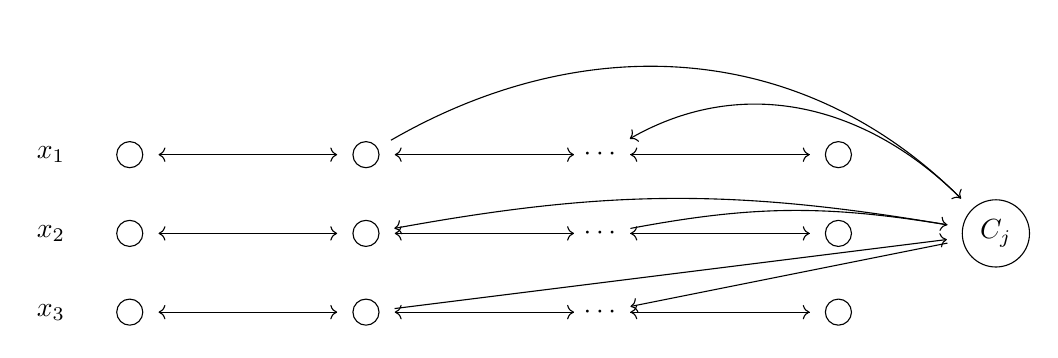
\begin{tikzpicture}

        \node[main] (Cj) at (8, -1) {$C_j$};

        \node (x1) at (-4, 0) {$x_1$};
        \node[main] (x11) at (-3, 0) {};
        \node[main] (x12) at (0, 0) {};
        \node (x1dots) at (3, 0) {$\cdots$};
        \node[main] (x1n) at (6, 0) {};

        \node (x2) at (-4, -1) {$x_2$};
        \node[main] (x21) at (-3, -1) {};
        \node[main] (x22) at (0, -1) {};
        \node (x2dots) at (3, -1) {$\cdots$};
        \node[main] (x2n) at (6, -1) {};

        \node (x3) at (-4, -2) {$x_3$};
        \node[main] (x31) at (-3, -2) {};
        \node[main] (x32) at (0, -2) {};
        \node (x3dots) at (3, -2) {$\cdots$};
        \node[main] (x3n) at (6, -2) {};

        \draw [->] (x11) -- (x12);
        \draw [->] (x12) -- (x11);
        \draw [->] (x12) -- (x1dots);
        \draw [->] (x1dots) -- (x12);
        \draw [->] (x1dots) -- (x1n);
        \draw [->] (x1n) -- (x1dots);

        \draw [->] (x21) -- (x22);
        \draw [->] (x22) -- (x21);
        \draw [->] (x22) -- (x2dots);
        \draw [->] (x2dots) -- (x22);
        \draw [->] (x2dots) -- (x2n);
        \draw [->] (x2n) -- (x2dots);

        \draw [->] (x31) -- (x32);
        \draw [->] (x32) -- (x31);
        \draw [->] (x32) -- (x3dots);
        \draw [->] (x3dots) -- (x32);
        \draw [->] (x3dots) -- (x3n);
        \draw [->] (x3n) -- (x3dots);

        \draw [->] (x12) to[out=30] (Cj);
        \draw [<-] (x1dots) to[out=30] (Cj);

        \draw [<-] (x22) to[bend left=10] (Cj);
        \draw [->] (x2dots) to[bend left=10] (Cj);

        \draw [->] (x32) -- (Cj);
        \draw [<-] (x3dots) -- (Cj);

      \end{tikzpicture}
    \end{center}

    We do this for every clause, connect the gadget to vertices $3j$ and $3j +
    1$.
  }

  \subsection*{Coping Intractability}

  Sometimes problems are hard, and we might not know it. Here's some things we
  can do.

  \begin{itemize}
    \item Hope they're not hard.
    \item Use an exponential time algorithm. For small instances, maybe that's
      ok.
    \item Find an efficient algorithm for special cases, maybe the cases you
      care about.

      For example on Homework 3, we gave a dynamic programming algorithm for the
      vertex cover problem on trees, instead of general graph. Maybe you can do
      it if a graph is ``not too far away from a tree."

    \item Maybe we can find a ``good enough" approximate solution.
  \end{itemize}

  \section{Approximation Algorithm}

  Consider an optimization problem. We can quantify the quality of an
  appropriate solution by the {\bf approximation ratio} $\gamma$.

  \begin{itemize}
    \item For a maximization problem, we want to find a solution with value $x$
      so that

      \[
        \frac{x}{\opt} \ge \gamma
      \]

      with $\gamma \le 1$, and $\opt$ is the optimal solution.

    \item For a minimization problem, we want to find a solution with value $x$
      so that

      \[
        \frac{x}{\opt} \le \gamma
      \]

      here with $\gamma \ge 1$.
  \end{itemize}

  \subsection{Load Balancing Problem}

  Given jobs $\{1, \dots, n\}$ where job $i$ takes time $t_i$. We want to assign
  each job to one of $m$ machines. Let $A_j$ be the set of jobs that we chose to
  assign to machine $j$. We get to chose what goes in this set.

  The load on machine $j$ is the total amount of time it will take to finish all
  jobs in $A_j$.

  \[
    \text{load}(j) = \sum_{i \in A_j} t_i
  \]

  {\bf Goal}: Minimize the maximum load on any given machine. In other words

  \[
    \min(\max_j (\text{load}(j)))
  \]

  We are going to do this by defining what jobs go in $A_j$. 

  This problem is NP-Hard, try to show it.

  \subsubsection{The Greedy Approach}

  Go through all the jobs (don't worry about the order for now), and assign each
  job to the machine with the lowest load so far.

  This algorithm will not produce the optimal solution. Try to find such an
  instance. On the other hand, it's never worse than twice as bad as the optimal
  solution! Let's see why.

  \Theorem {
    The greedy algorithm achieves an approximation ratio of 2.
  }
  {
    \TODO{} Next time! :)
  }

\end{document}
